\section{Data and Monte Carlo simulations samples}
%\begin{tcolorbox}[breakable,colback=black!5!white,colframe=red!80!black,width=\textwidth]
%\chapter*{Data and Monte Carlo samples}
%\end{tcolorbox}
\label{sec:samples}

\subsection{Signal samples}

Signal samples of a spin-2 (bulk graviton) decaying into a pair of \Z bosons have been generated to design the analysis. To target the final state, one of the two \Z bosons is forced to decay into neutrinos, while the other \Z is forced to decay hadronically. The signal samples are produced in the narrow-width approximation by setting the resonance width to 0.1\% of its mass. Twelve mass points with 100000 events each are simulated, with a $m_{\G}$ ranging from 600 \GeV up to 4500 \GeV.

\noindent Additionally, samples of a spin-1 HVT-like \Wp resonance decaying into a \Z boson and a \W boson are studied. The \Z boson is forced to decay into neutrinos, and the \W boson is forced to decay hadronically. Also in this case the signal samples are produced in the narrow-width approximation by setting the resonance with to 0.1\% of its mass. Twelve mass points with 100000 events each are simulated, with a $m_{\Wp}$ ranging from 600 \GeV up to 4500 \GeV.

\noindent The signal samples are generated at leading-order (LO) with the {\sc MadGraph5\_aMCatNLO v 2.2.2}~\cite{bib:MADGRAPH} matrix element generator, while hadronization and fragmentation are handled by \PYTHIA 8~\cite{bib:PYTHIA} version 8.2121 with CUETP8M1~\cite{bib:CUETP8M1} tuning. A full detector simulation and event reconstruction has been performed with \GEANTfour~\cite{bib:GEANT4} and CMSSW. The detector alignement scenario, calibrations and pile-up distributions are generated according to the expectations in 2016 data.
%All signal samples belong to the {\tt RunIISummer16MiniAODv2\_PUMoriond17-80X\_mcRun2} campaign.

\noindent All the signal samples used in the analysis and the related properties are reported in Tables~\ref{tab:signal_samples}-\ref{tab:signal_samples_W}.
%Missing W'
%and ~\ref{tab:signal_samples_W}. 
 
 \begin{table}[!htb]
   \begin{center}
   \caption{Spin-2 (bulk graviton) signal samples and production cross sections (assumed to be 1 $\pb$) multiplied by the respective branching fractions of the \Z decays considered ($\mathcal{B}(\Z \to \nu\nu) = 0.20$, $\mathcal{B}(\Z \to qq) = 0.6991$). A combinatorial factor of 2 is included in the cross-section calculation. \label{tab:signal_samples}}
   \begin{tabular}{l|ccc}
 Signal process &  $m_{\G}$ & Events & $\sigma\times\mathcal{B}$ (\pb) \\
 \hline 
 \hline 
\BGinv & 600 GeV & 100000 & 0.27964\\
\BGinv & 800 GeV  & 100000 & 0.27964\\
\BGinv & 1000 GeV  & 100000 & 0.27964\\
\BGinv & 1200 GeV  & 100000 & 0.27964\\
\BGinv & 1400 GeV  & 100000 & 0.27964\\
\BGinv & 1800 GeV  & 100000 & 0.27964\\
\BGinv & 2000 GeV  & 100000 & 0.27964\\
\BGinv & 2500 GeV  & 100000 & 0.27964\\
\BGinv & 3000 GeV  & 100000 & 0.27964\\
\BGinv & 3500 GeV  & 100000 & 0.27964\\
\BGinv & 4000 GeV  & 100000 & 0.27964\\
\BGinv & 4500 GeV  & 100000 & 0.27964\\
   \end{tabular}
   \end{center}
 \end{table}

 \begin{table}[!htb]
   \begin{center}
   \caption{Spin-1 (W') signal samples and production cross sections (assumed to be 1 $\pb$) multiplied by the \Z and \W branching fraction ($\mathcal{B}(\Z \to \nu\nu) = 0.2$, $\mathcal{B}(\W \to qq) = 0.6760$).\label{tab:signal_samples_W}}
   \begin{tabular}{l|ccc}
 Signal process &  $m_{\Wp}$ & Events & $\sigma\times\mathcal{B}$ (\pb) \\
 \hline
 \hline 
\Wpinv & 600 GeV & 100000 & 0.13482\\
\Wpinv & 800 GeV  & 100000 & 0.13482\\
\Wpinv & 1000 GeV  & 100000 & 0.13482\\
\Wpinv & 1200 GeV  & 100000 & 0.13482\\
\Wpinv & 1400 GeV  & 100000 & 0.13482\\
\Wpinv & 1800 GeV  & 100000 & 0.13482\\
\Wpinv & 2000 GeV  & 100000 & 0.13482\\
\Wpinv & 2500 GeV  & 100000 & 0.13482\\
\Wpinv & 3000 GeV  & 100000 & 0.13482\\
\Wpinv & 3500 GeV  & 100000 & 0.13482\\
\Wpinv & 4000 GeV  & 100000 & 0.13482\\
\Wpinv & 4500 GeV  & 100000 & 0.13482\\
   \end{tabular}
   \end{center}

 \end{table}


\subsection{Signal characterization}

This analysis is performed in a high mass region (from 1~\TeV to 4.5~\TeV). %The \MADGRAPH algorithm generates the hard process production in the collision with \pt = 0. In the next step of the simulation, during the hadronization, \PYTHIA adds the QCD ISR (initial state radiation) and consequently the resonance \pt different from 0.
The \MADGRAPH algorithm generates the hard process production in the collision. In the next step of the simulation, during the hadronization, \PYTHIA adds the QCD ISR (initial state radiation). 
%The transverse mass and \pt distributions of the heavy resonance after the \PYTHIA simulation are shown in fig.~\ref{fig:genSignal1} for bulk graviton signal samples (and in fig.~\ref{fig:genSignal2} for \Wp signal samples). The typical \pt is small compared to the mass of the resonance, and about two thirds of the events have \pt smaller than 50 \GeV. The \pt distributions of the electroweak bosons, along with the mass of the hadronically decaying \Z (\W) and the angular separation of the two electroweak bosons in the transverse plane are shown as well.
Kinematical distributions at generator level are shown in fig.~\ref{fig:genGravSignal1}-\ref{fig:genGravSignal3} for spin-2 bulk graviton signal, and in fig.~\ref{fig:genWprimeSignal1}-\ref{fig:genWprimeSignal3} for spin-1 HVT \Wp signal.

 \begin{figure}[!htb]
   \begin{center}
     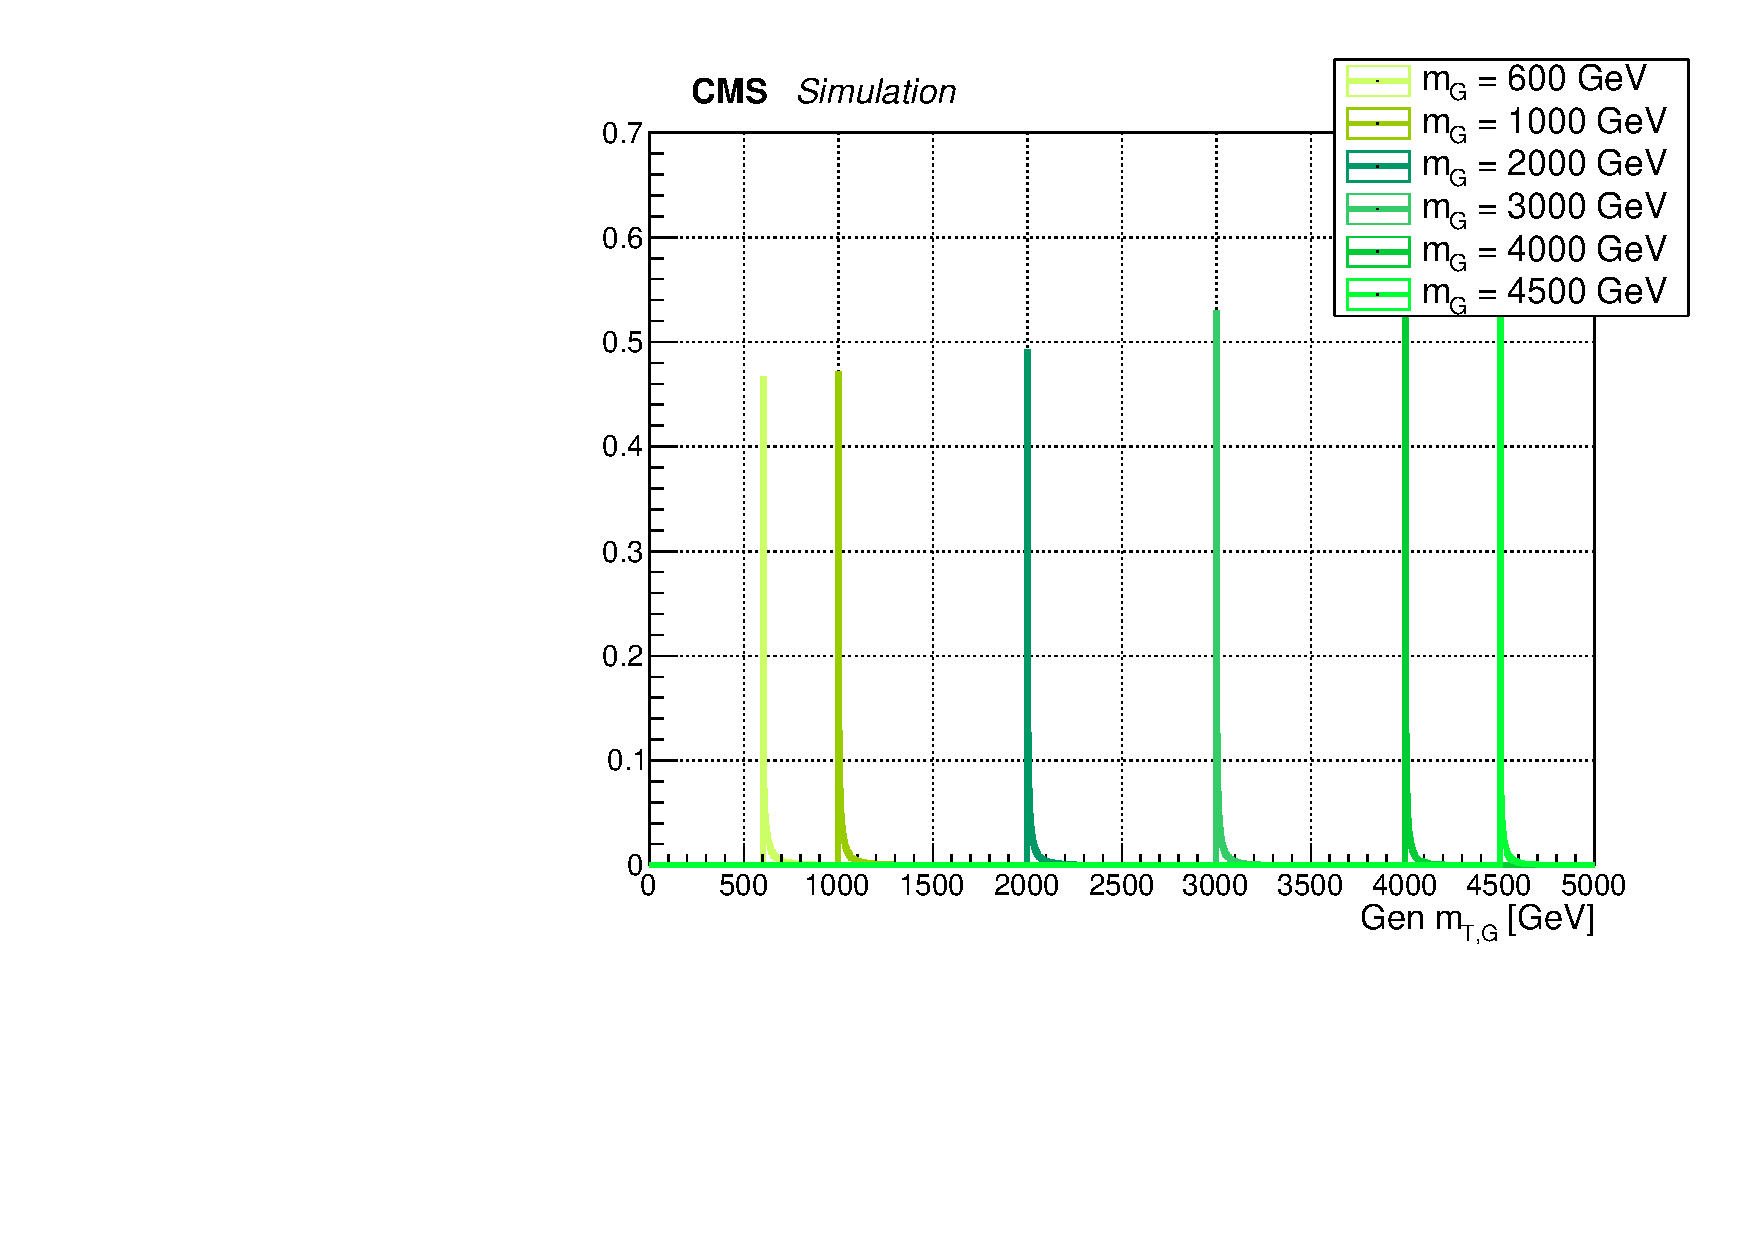
\includegraphics[width=.495\textwidth]{Gen_v9/XZZInv_g_XMT.pdf}%GenPhi1pt.pdf}
     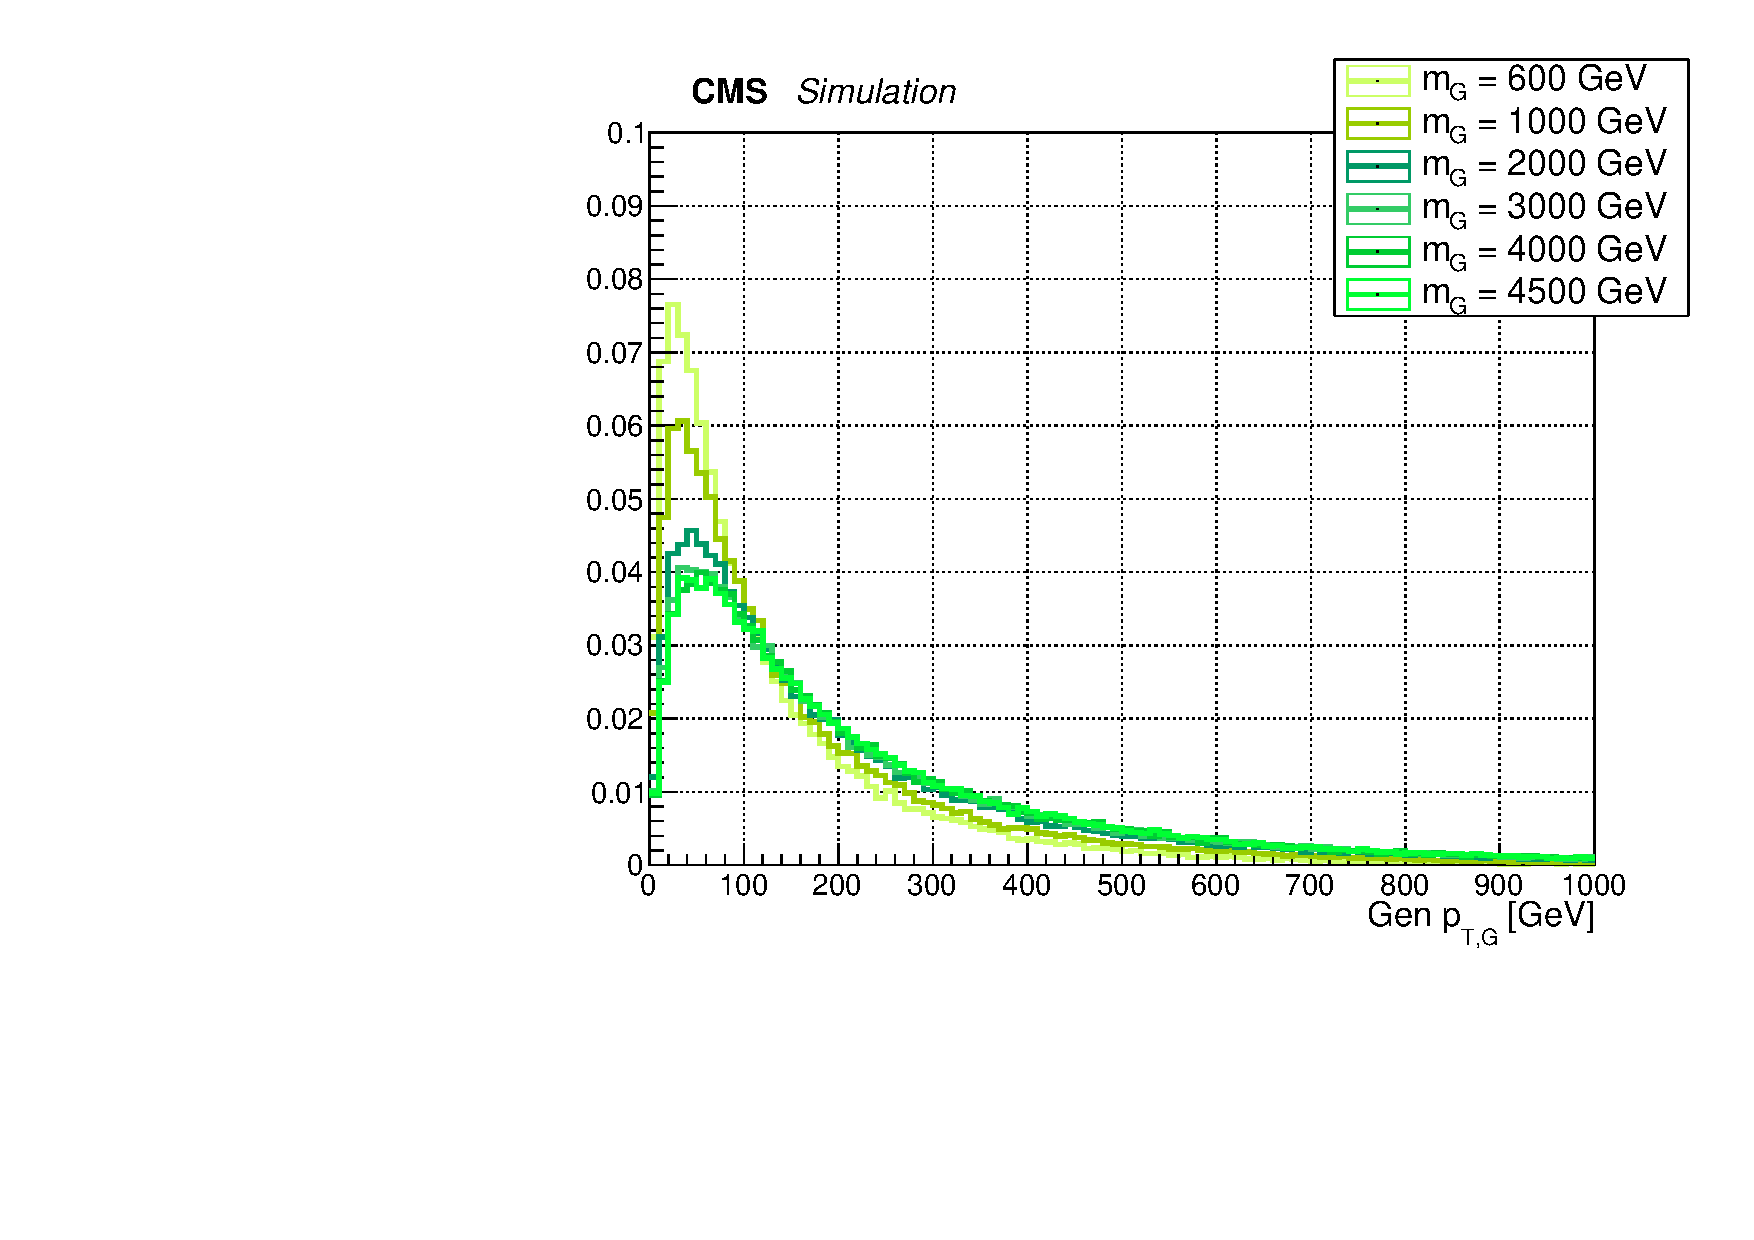
\includegraphics[width=.495\textwidth]{Gen_v9/XZZInv_g_XPt.pdf}%GenPhi1y.pdf}
     %\\
     %\includegraphics[width=.495\textwidth]{Gen_v7/g_ZLepMass.pdf}%GenZmass.pdf}
     %\includegraphics[width=.495\textwidth]{Gen_v7/g_ZHadMass.pdf}%GenHmass.pdf}
     \\
     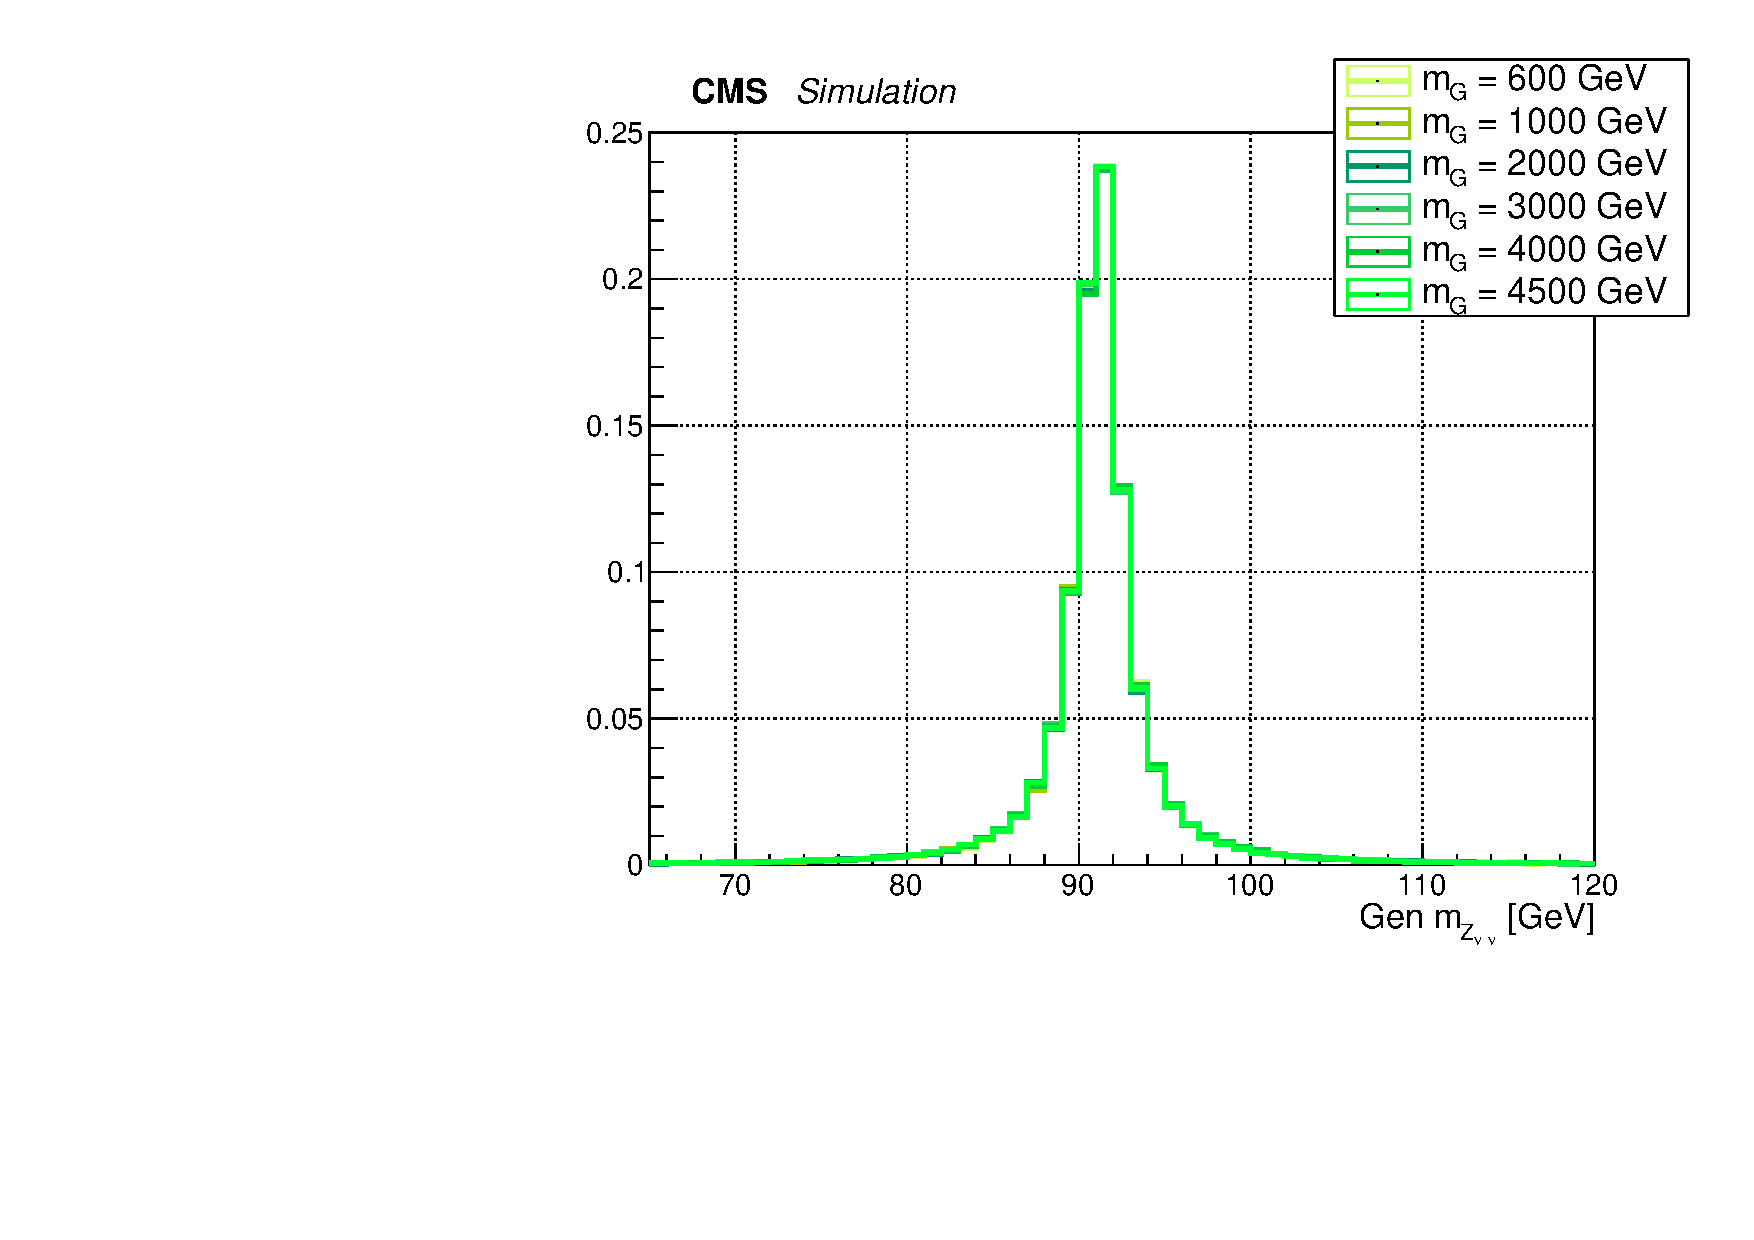
\includegraphics[width=.495\textwidth]{Gen_v9/XZZInv_g_ZLepMass.pdf}%GenZpt.pdf}
     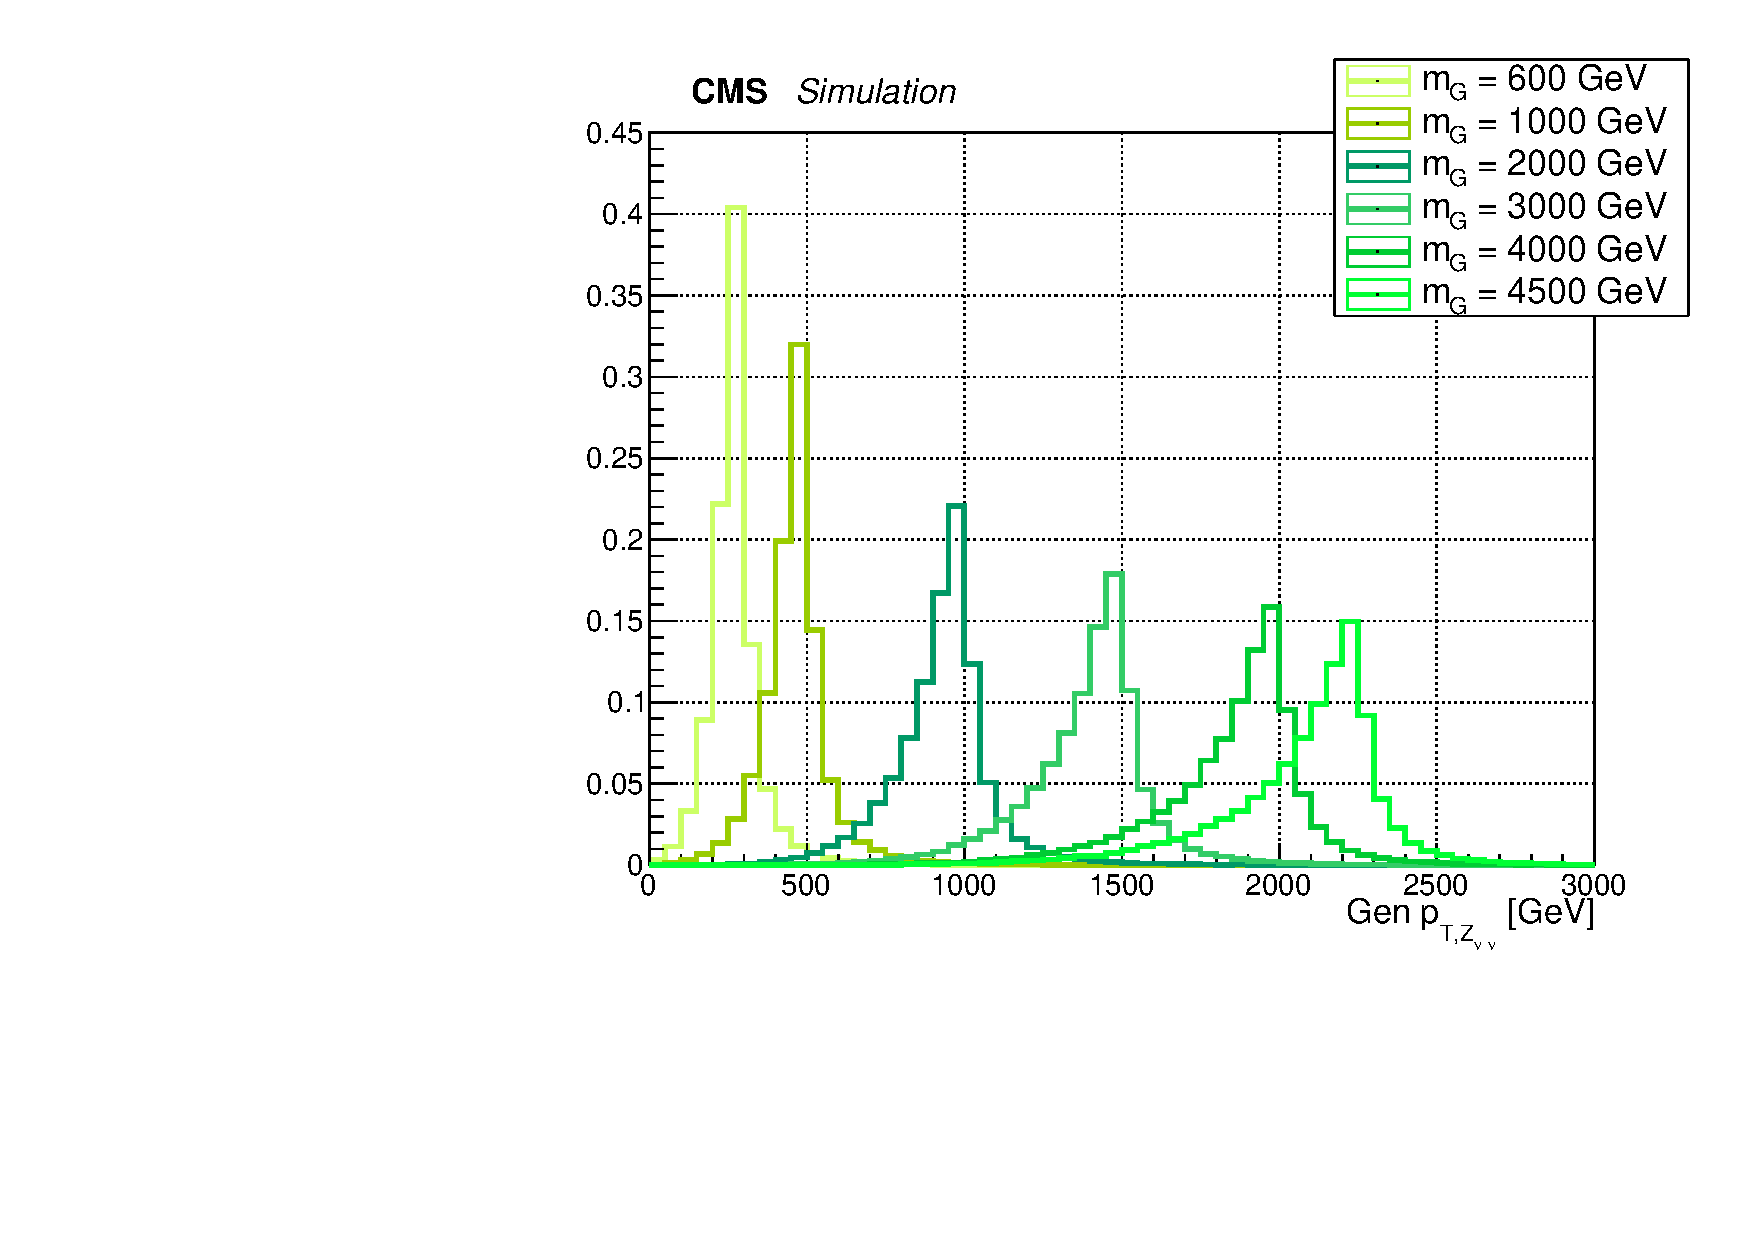
\includegraphics[width=.495\textwidth]{Gen_v9/XZZInv_g_ZLepPt.pdf}%GenHpt.pdf}
     \\
     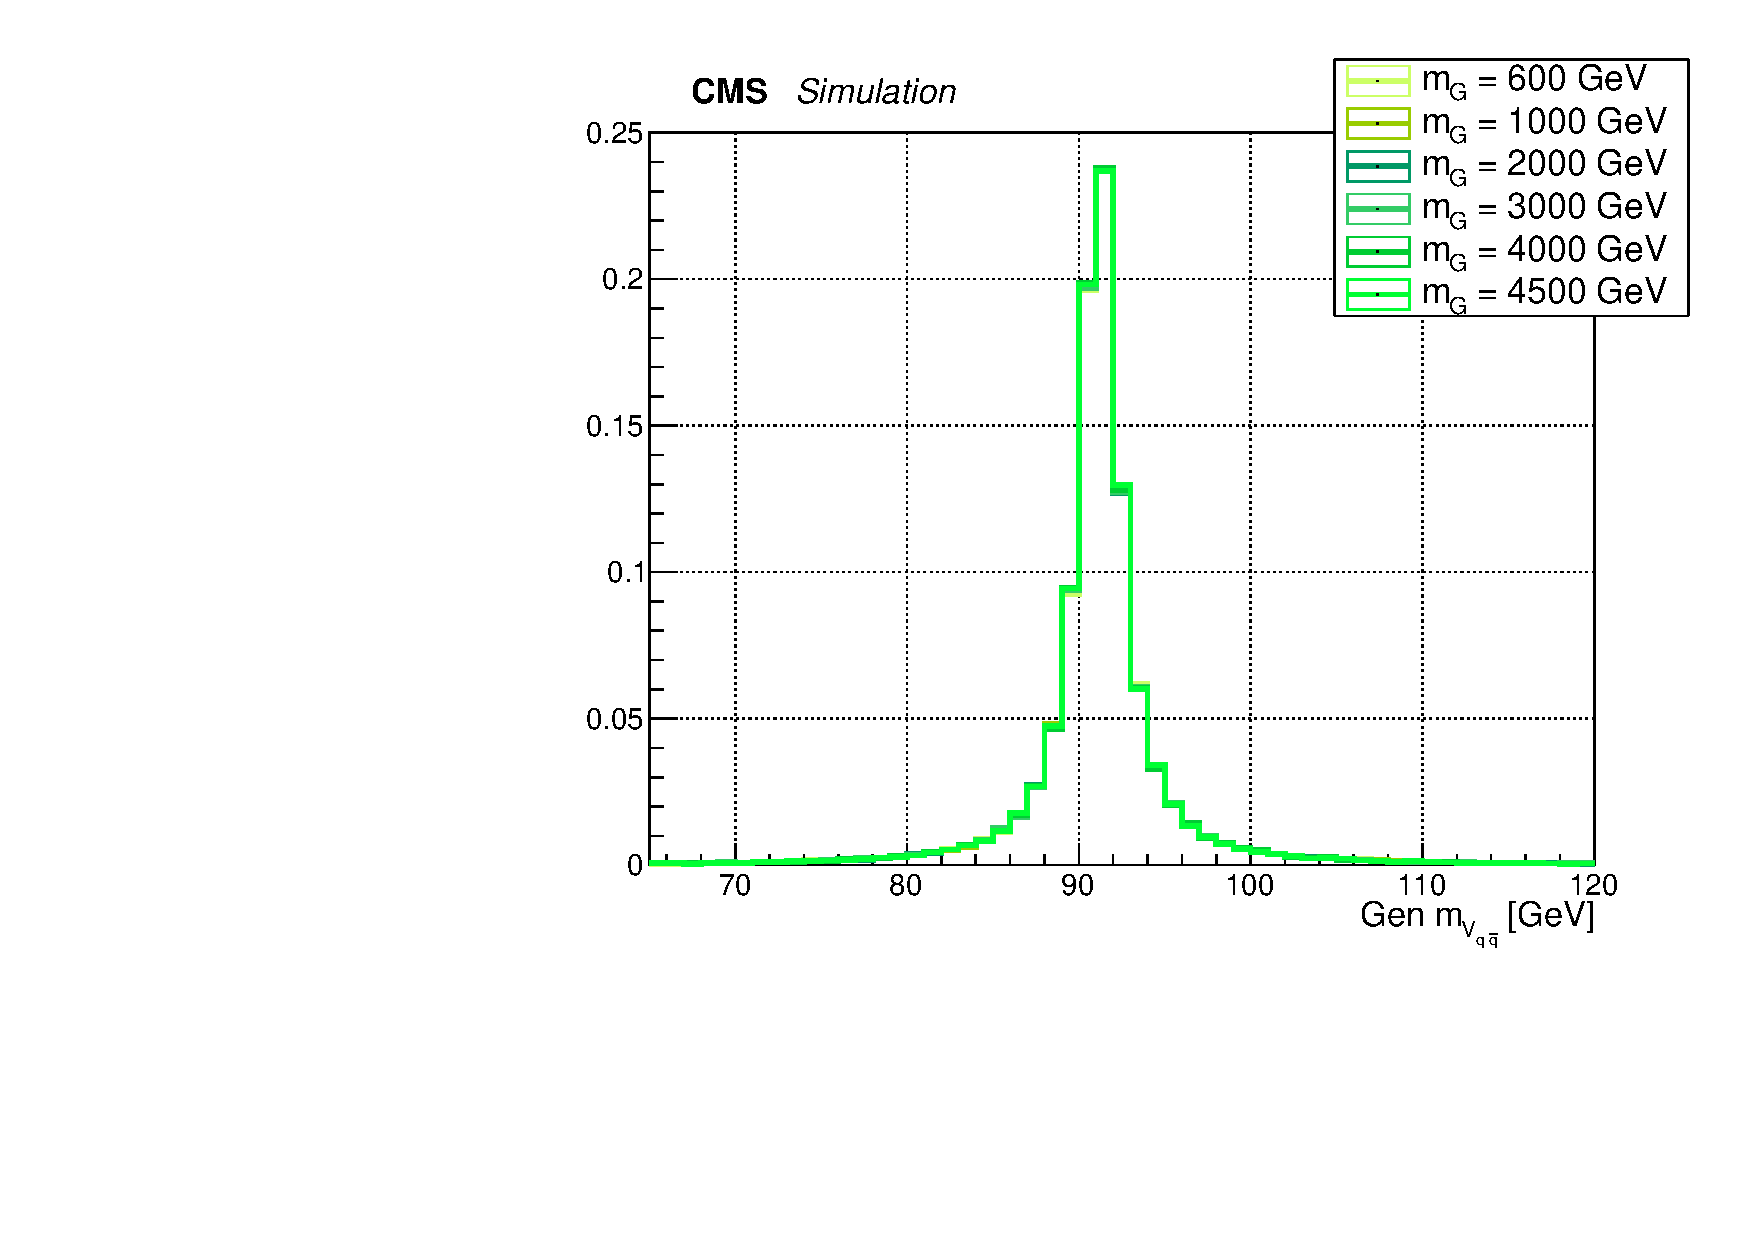
\includegraphics[width=.495\textwidth]{Gen_v9/XZZInv_g_VHadMass.pdf}%GenZdR.pdf}
     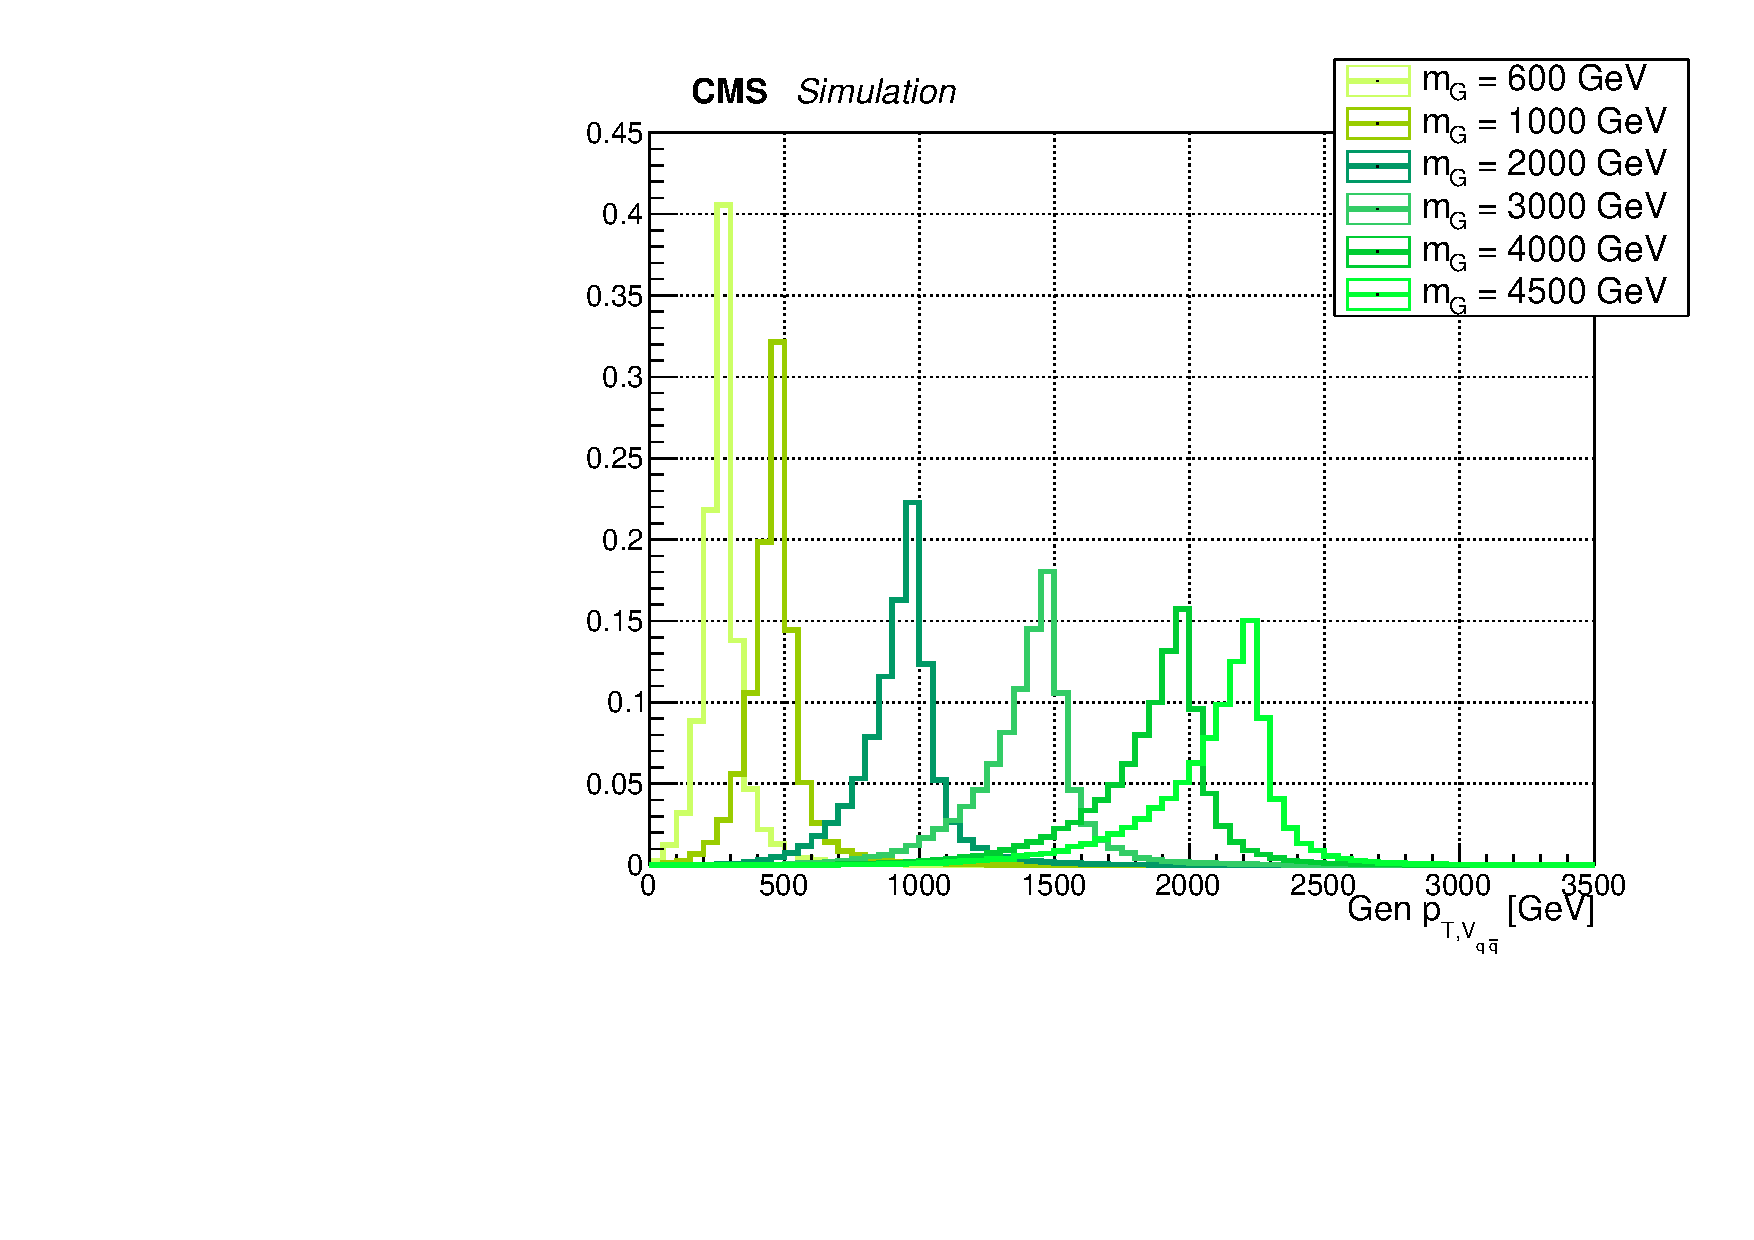
\includegraphics[width=.495\textwidth]{Gen_v9/XZZInv_g_VHadPt.pdf}%GenHdR.pdf}
   \end{center}
   \caption{Main signal kinematic quantities at generation level after parton showering, for spin-2 bulk graviton signal, considering different mass hypoteses ($m_{\G} = 0.6, 1, 2, 3, 4, 4.5$ TeV). Top: graviton transverse mass and \pt distributions. Center: invisibly decaying \Z mass and \pt. Bottom: hadronically decaying \Z mass and \pt.}
   \label{fig:genGravSignal1}
 \end{figure}

 \begin{figure}[!htb]
   \begin{center}
     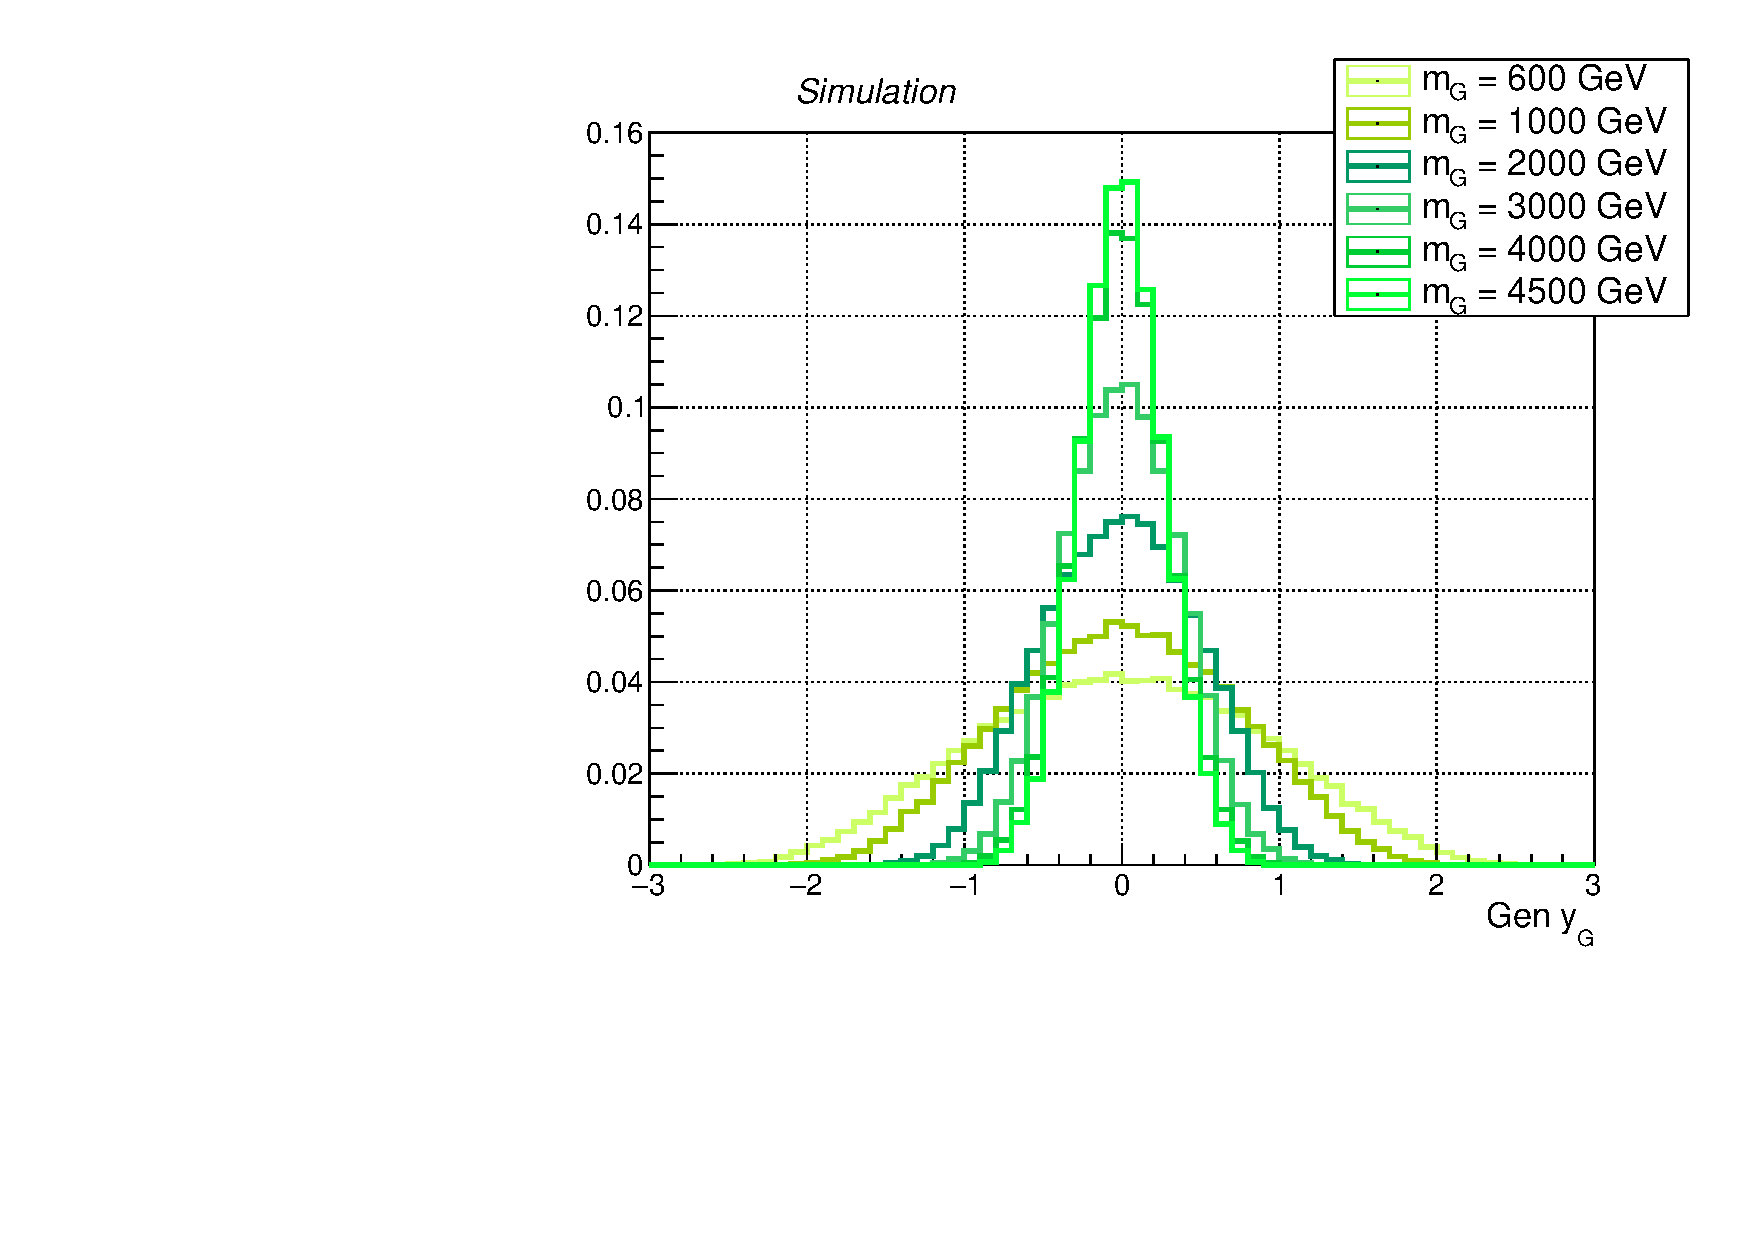
\includegraphics[width=.495\textwidth]{Gen_v9/XZZInv_g_XRapidity.pdf}%GenPhi1pt.pdf}
     %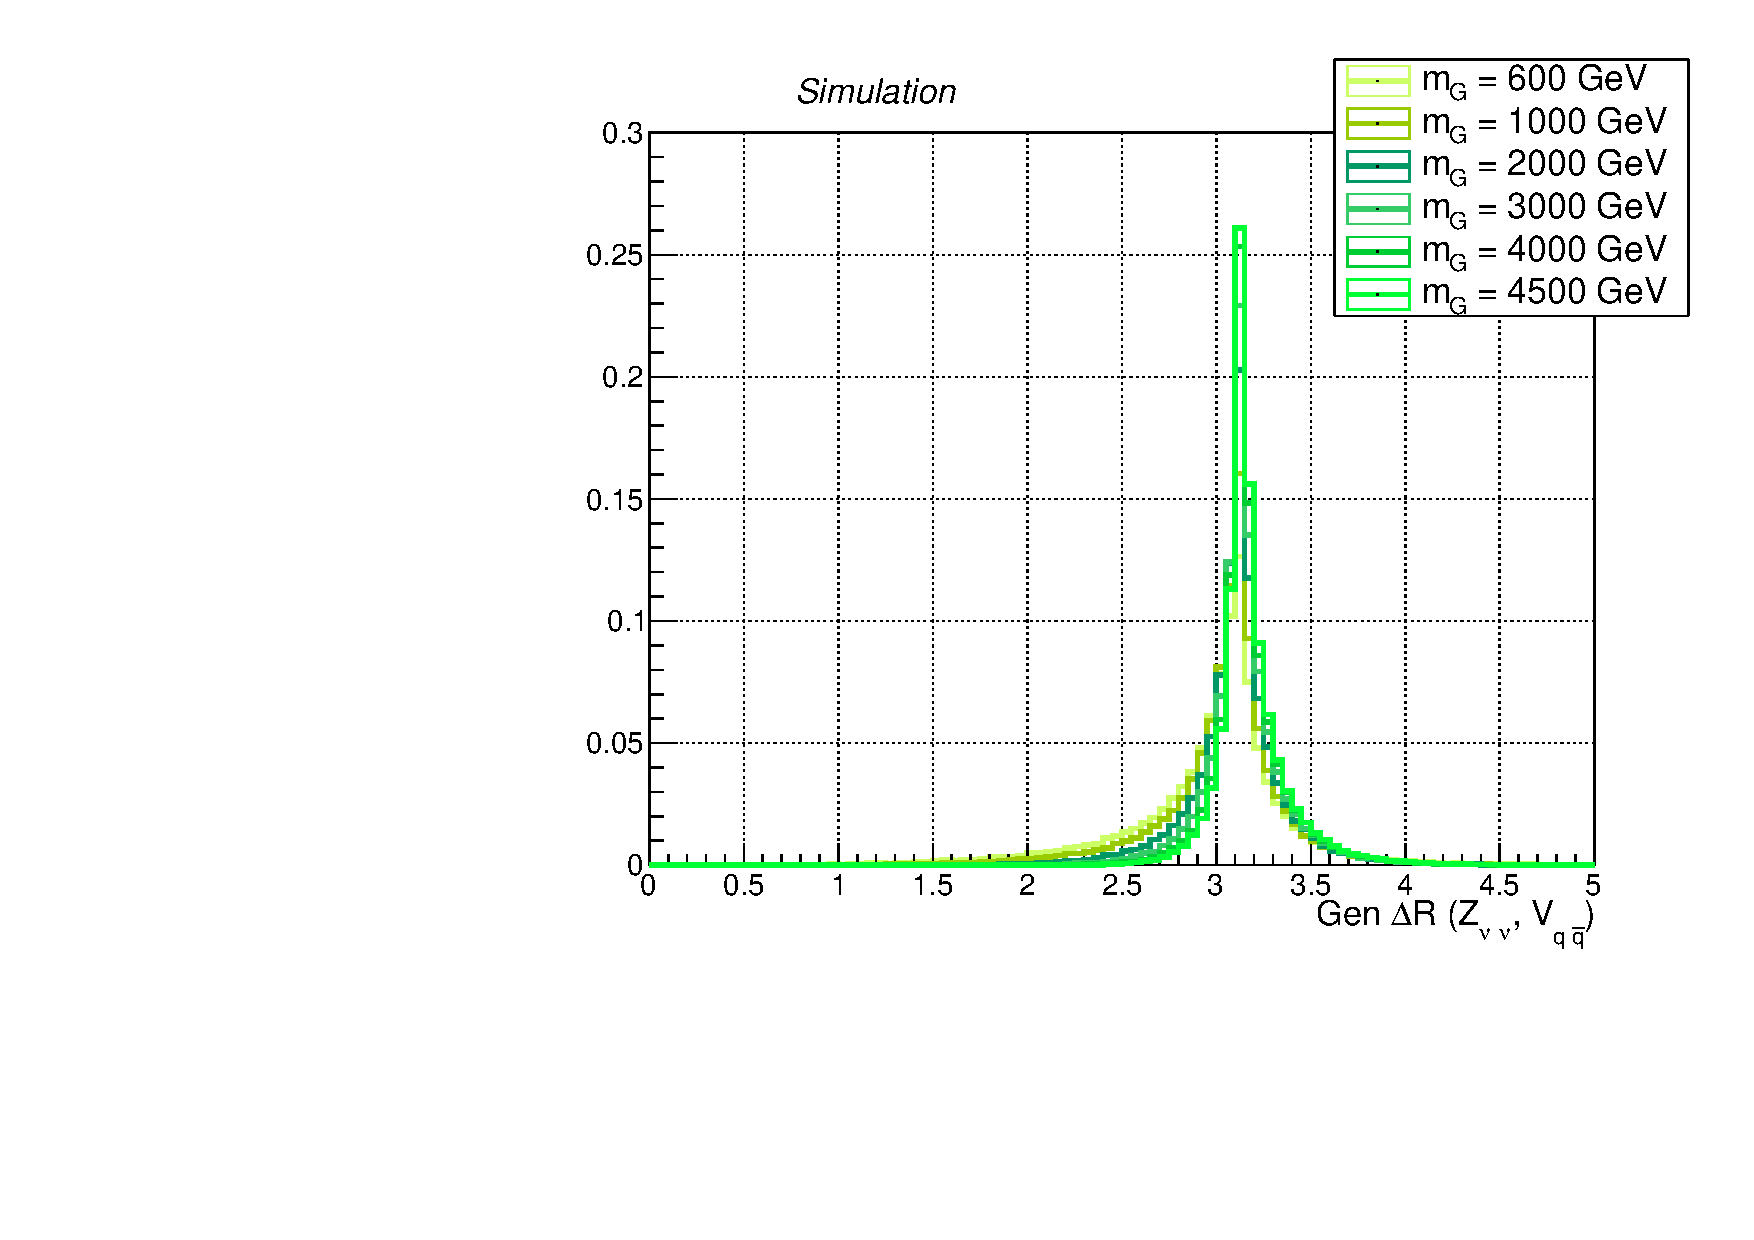
\includegraphics[width=.495\textwidth]{Gen_v9/XZZInv_g_VZDR.pdf}%GenPhi1y.pdf}
     %\\
     %\includegraphics[width=.495\textwidth]{Gen_v7/g_ZLepMass.pdf}%GenZmass.pdf}
     %\includegraphics[width=.495\textwidth]{Gen_v7/g_ZHadMass.pdf}%GenHmass.pdf}
     \\
     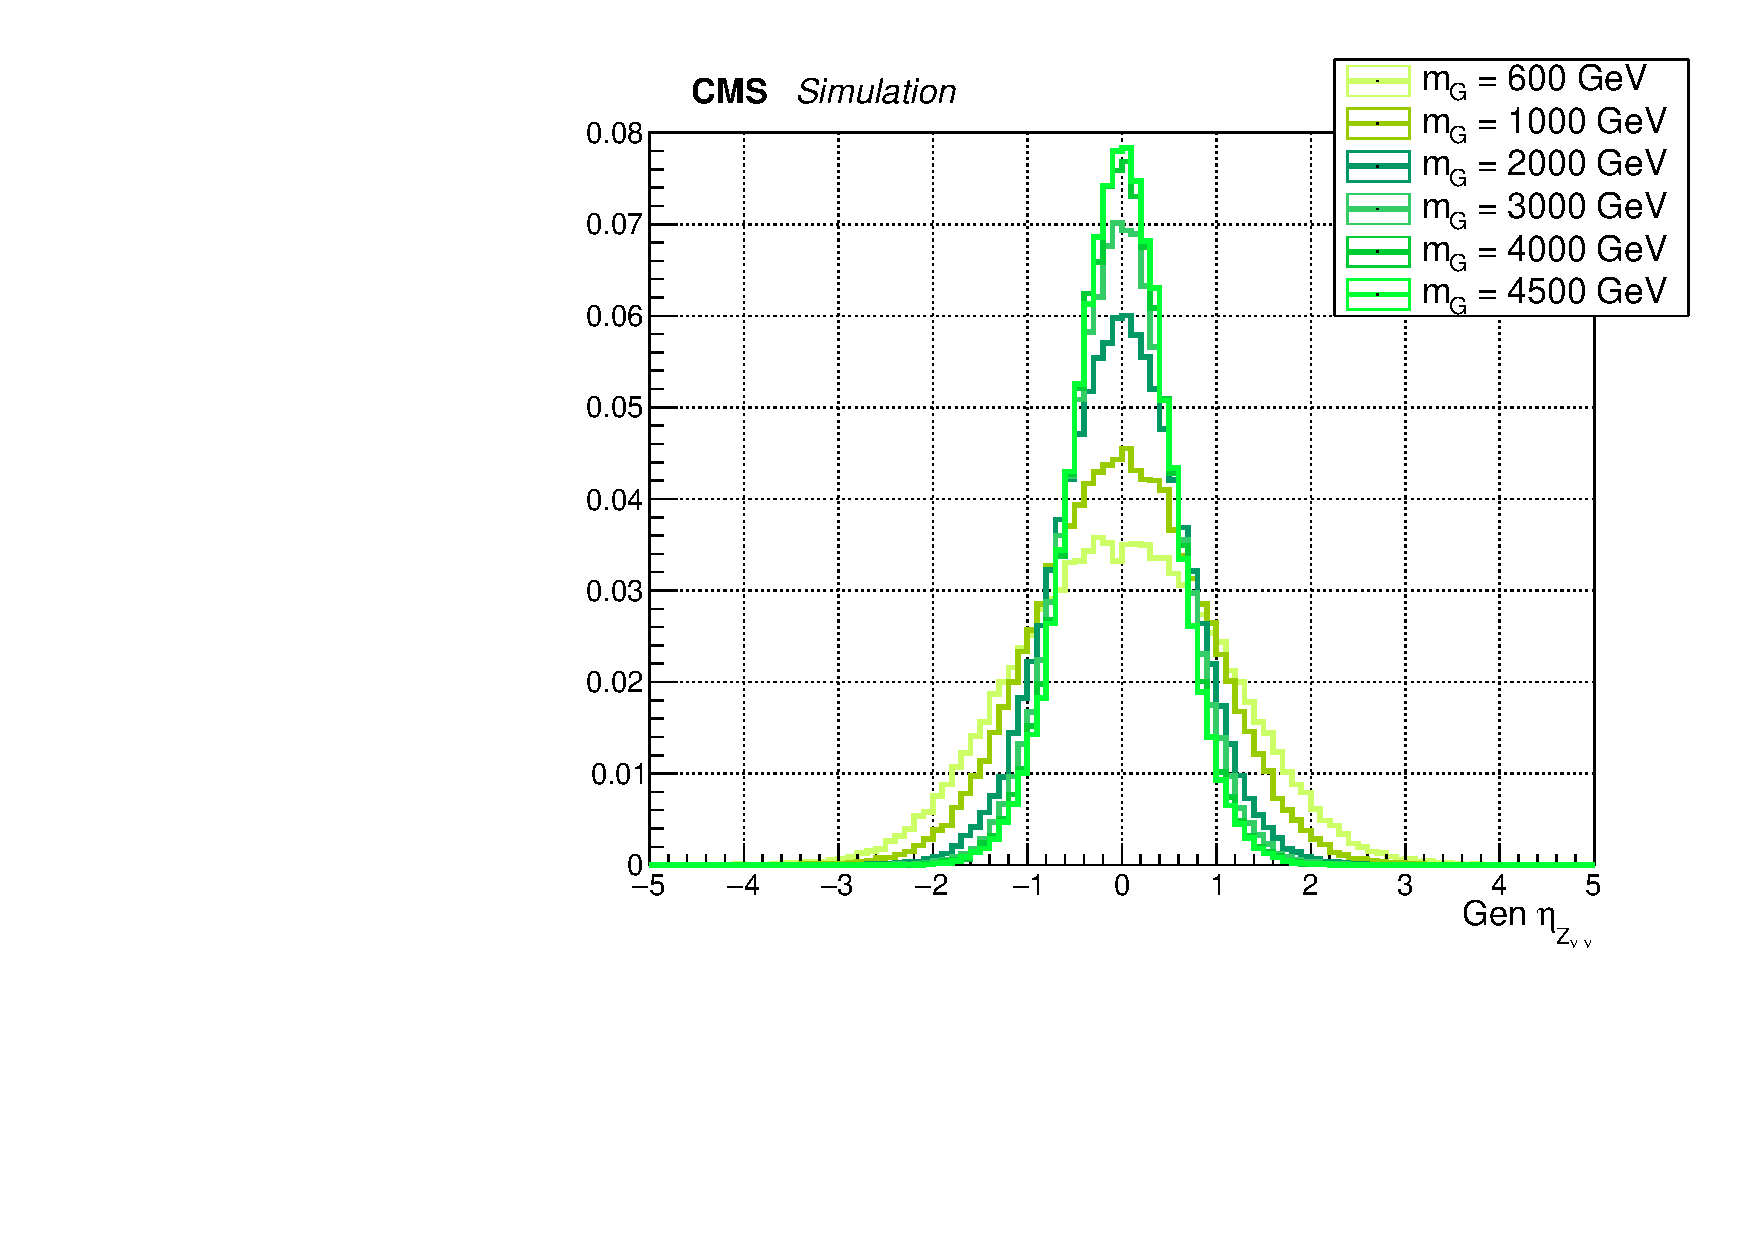
\includegraphics[width=.495\textwidth]{Gen_v9/XZZInv_g_ZLepEta.pdf}%GenZpt.pdf}
     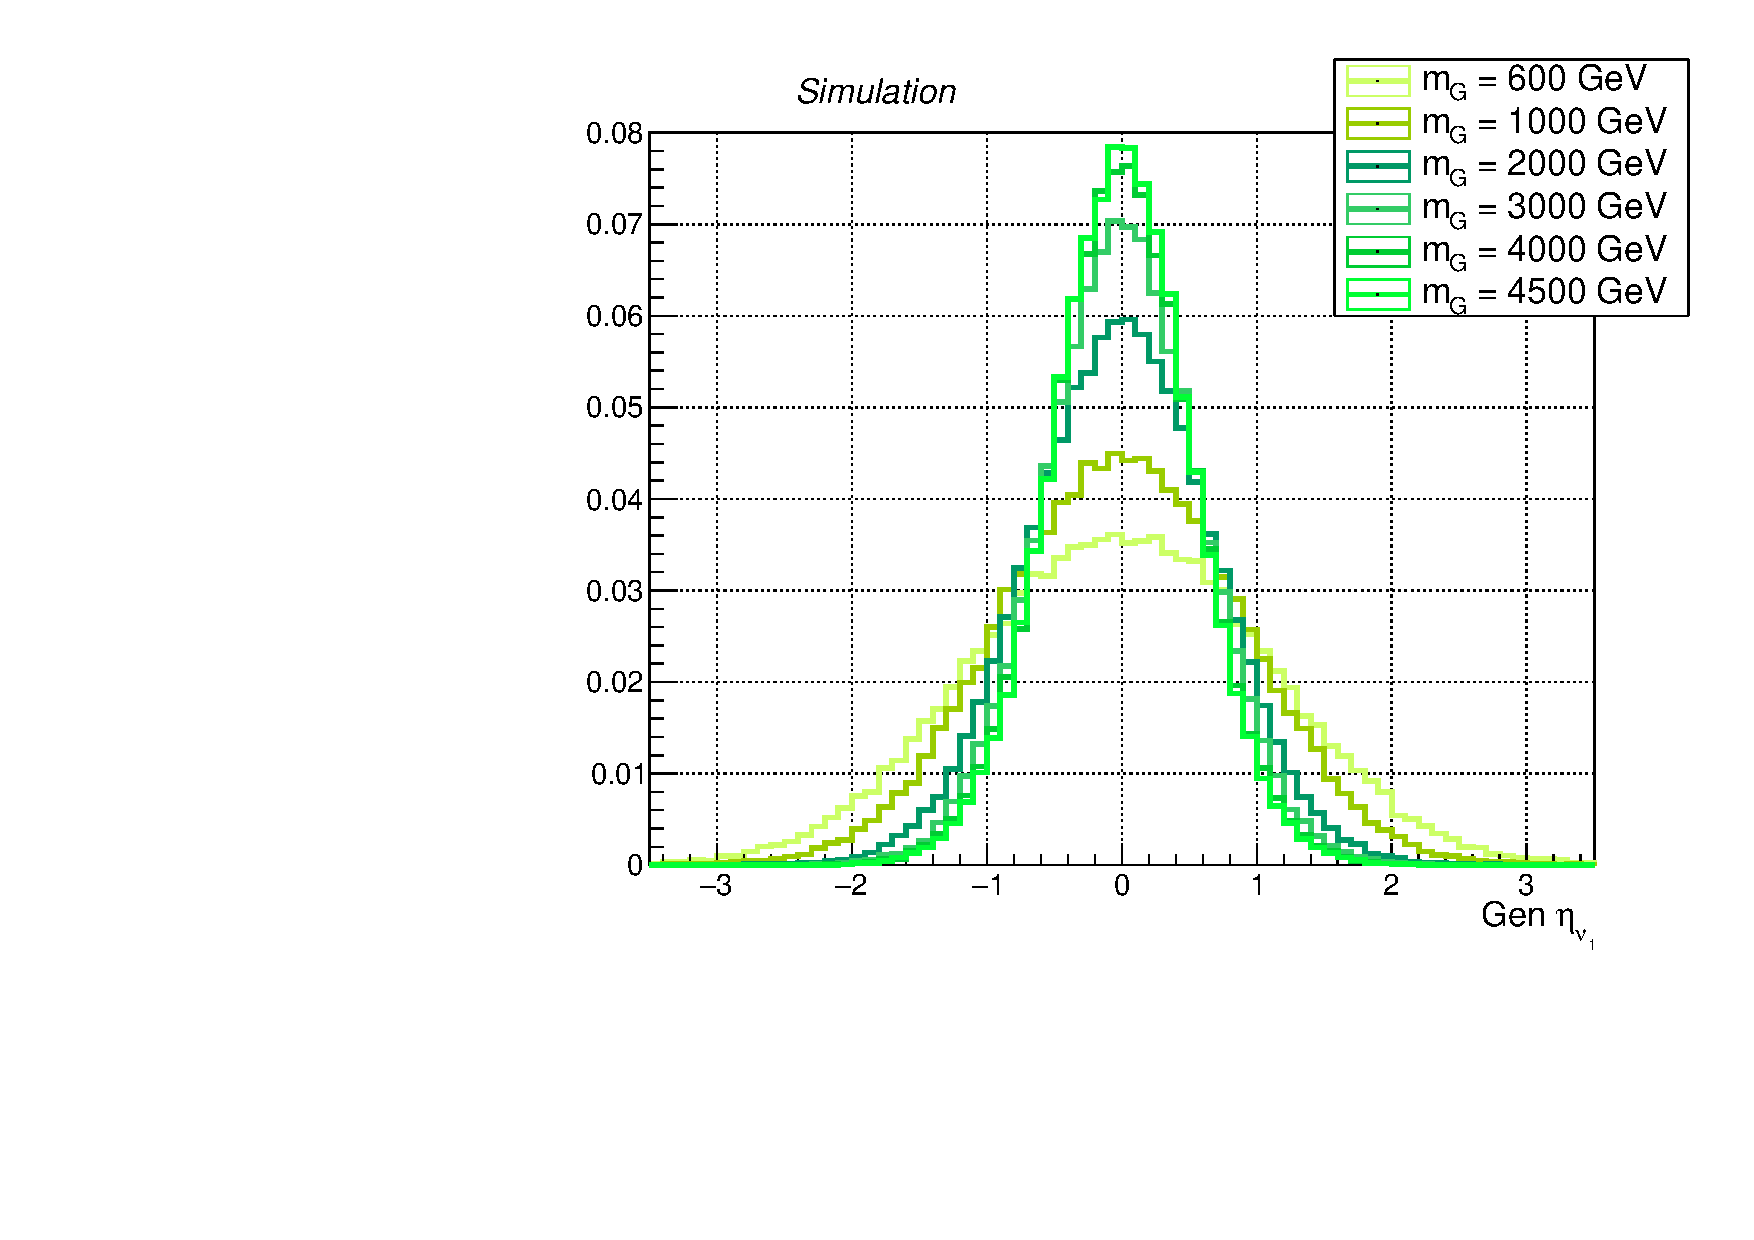
\includegraphics[width=.495\textwidth]{Gen_v9/XZZInv_g_Lep1Eta.pdf}%GenHpt.pdf}
     \\
     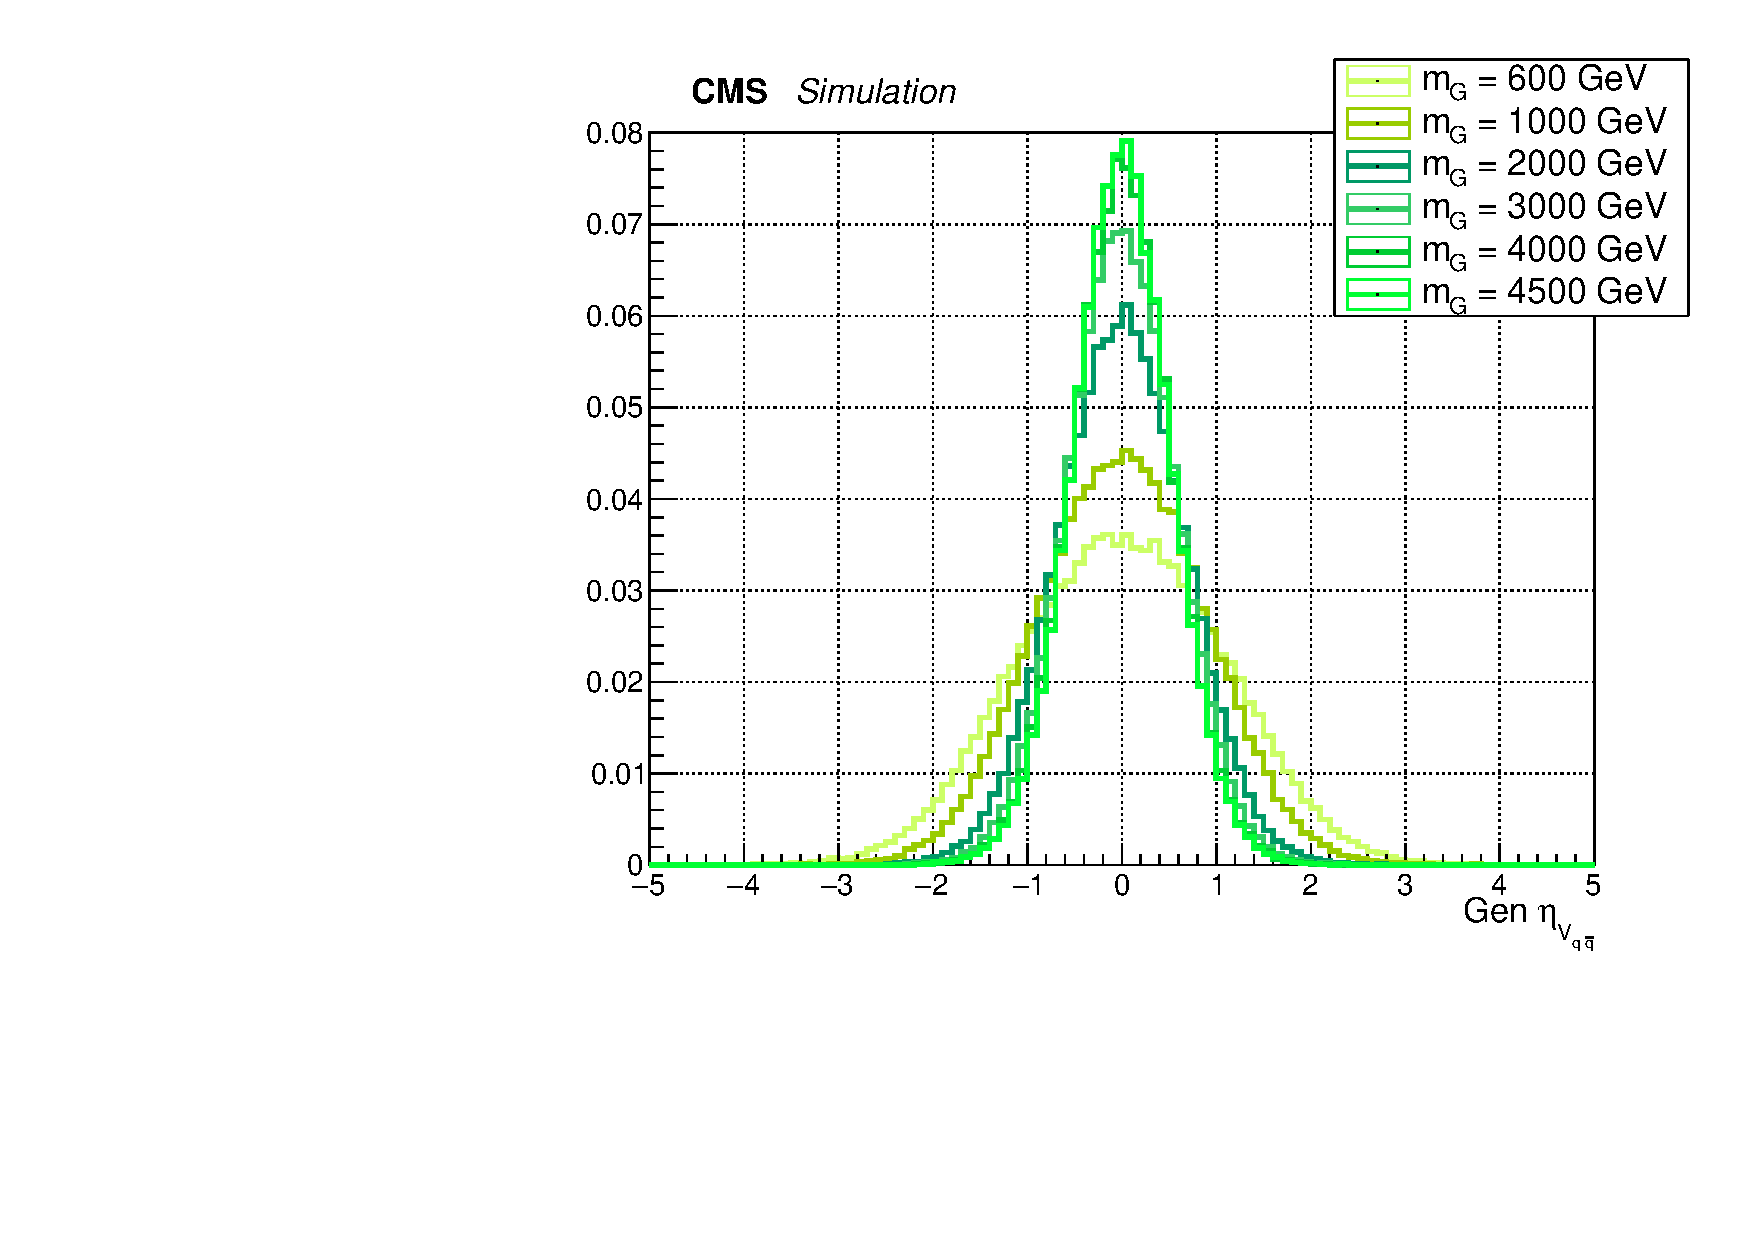
\includegraphics[width=.495\textwidth]{Gen_v9/XZZInv_g_VHadEta.pdf}%GenZdR.pdf}
     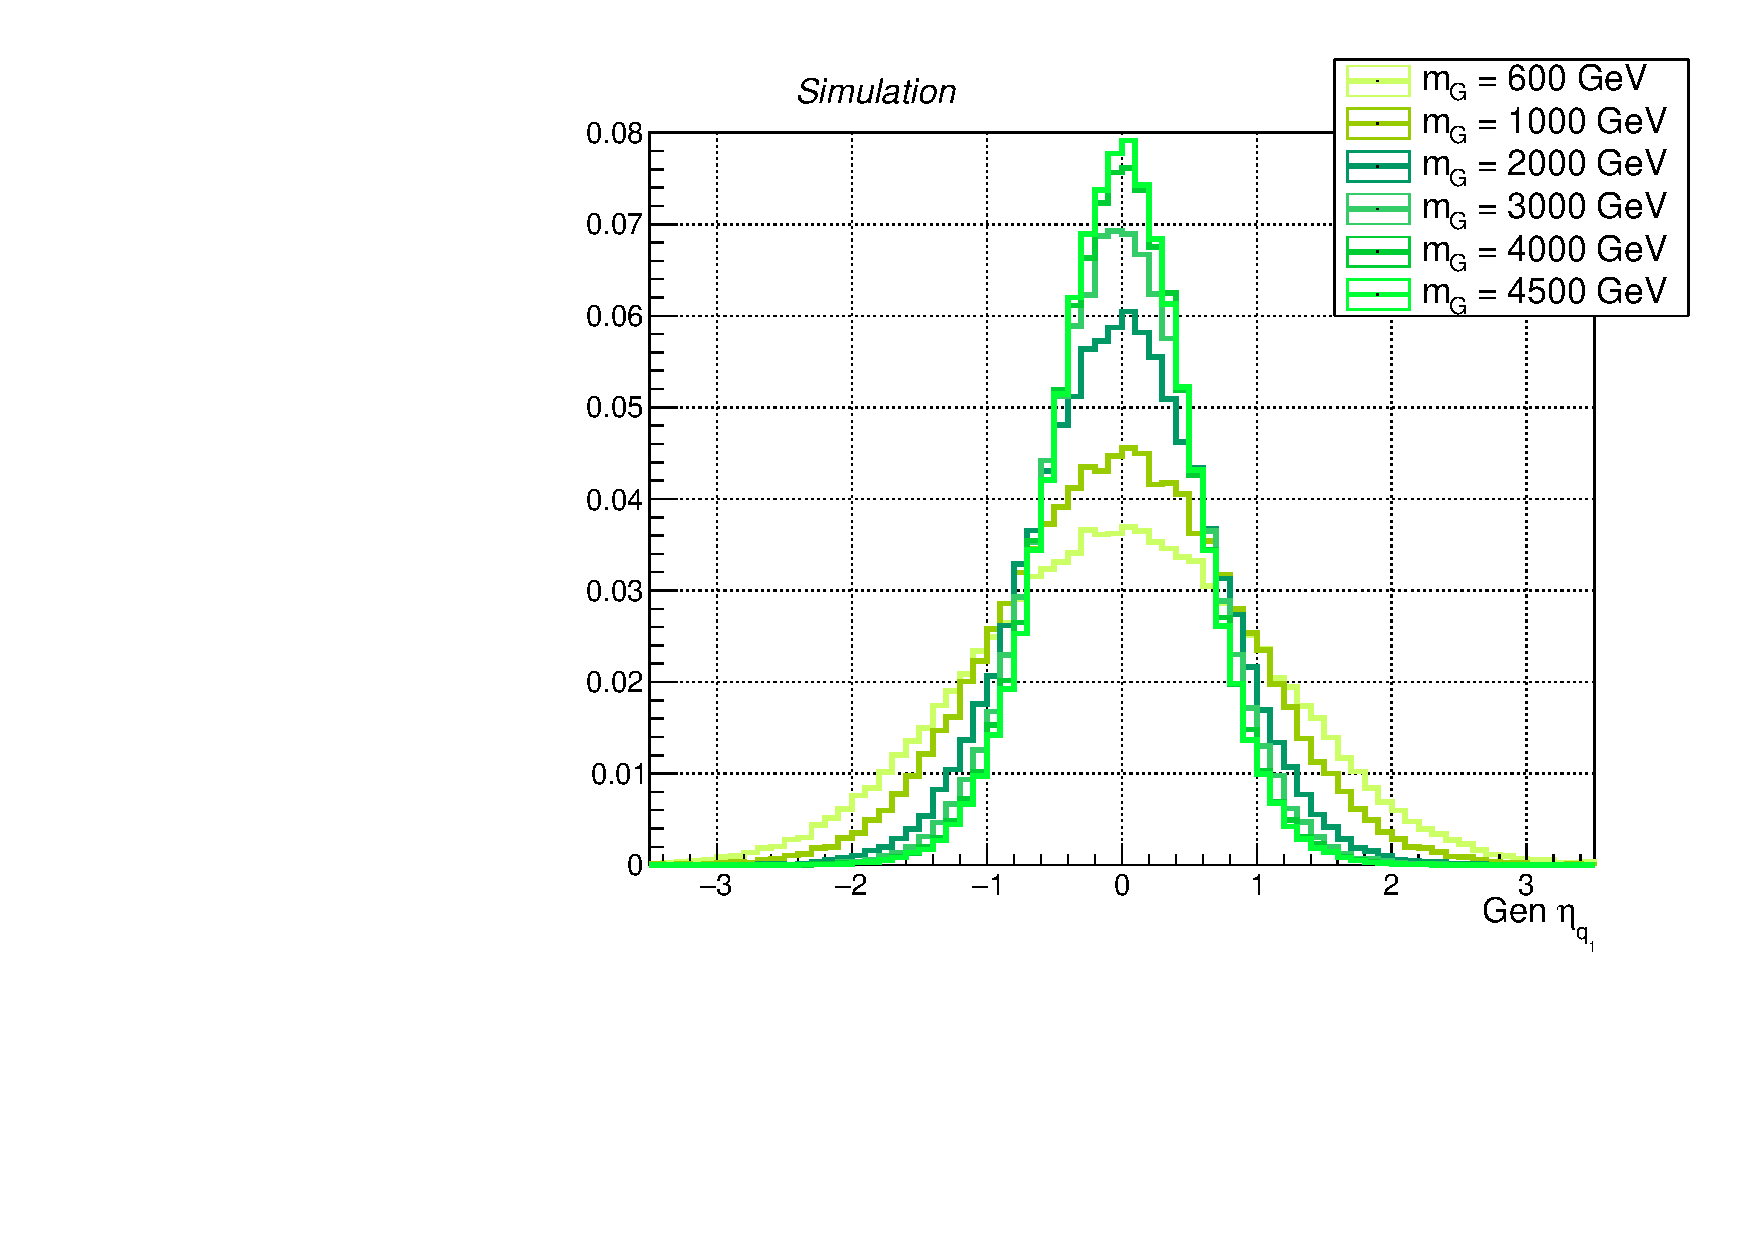
\includegraphics[width=.495\textwidth]{Gen_v9/XZZInv_g_Had1Eta.pdf}%GenHdR.pdf}
   \end{center}
   \caption{Main signal kinematic quantities at generation level after parton showering, for spin-2 bulk graviton signal, considering different mass hypoteses ($m_{\G} = 0.6, 1, 2, 3, 4, 4.5$ TeV). Top: graviton rapidity $\mathcal{Y}$. Center: pseudorapidity $\eta$ of the invisibly decaying \Z, and pseudorapidity of the leading neutrino. Bottom: pseudorapidity $\eta$ of the hadronically decaying \Z, and pseudorapidity of the leading quark.}
   \label{fig:genGravSignal2}
 \end{figure}

 \begin{figure}[!htb]
   \begin{center}
     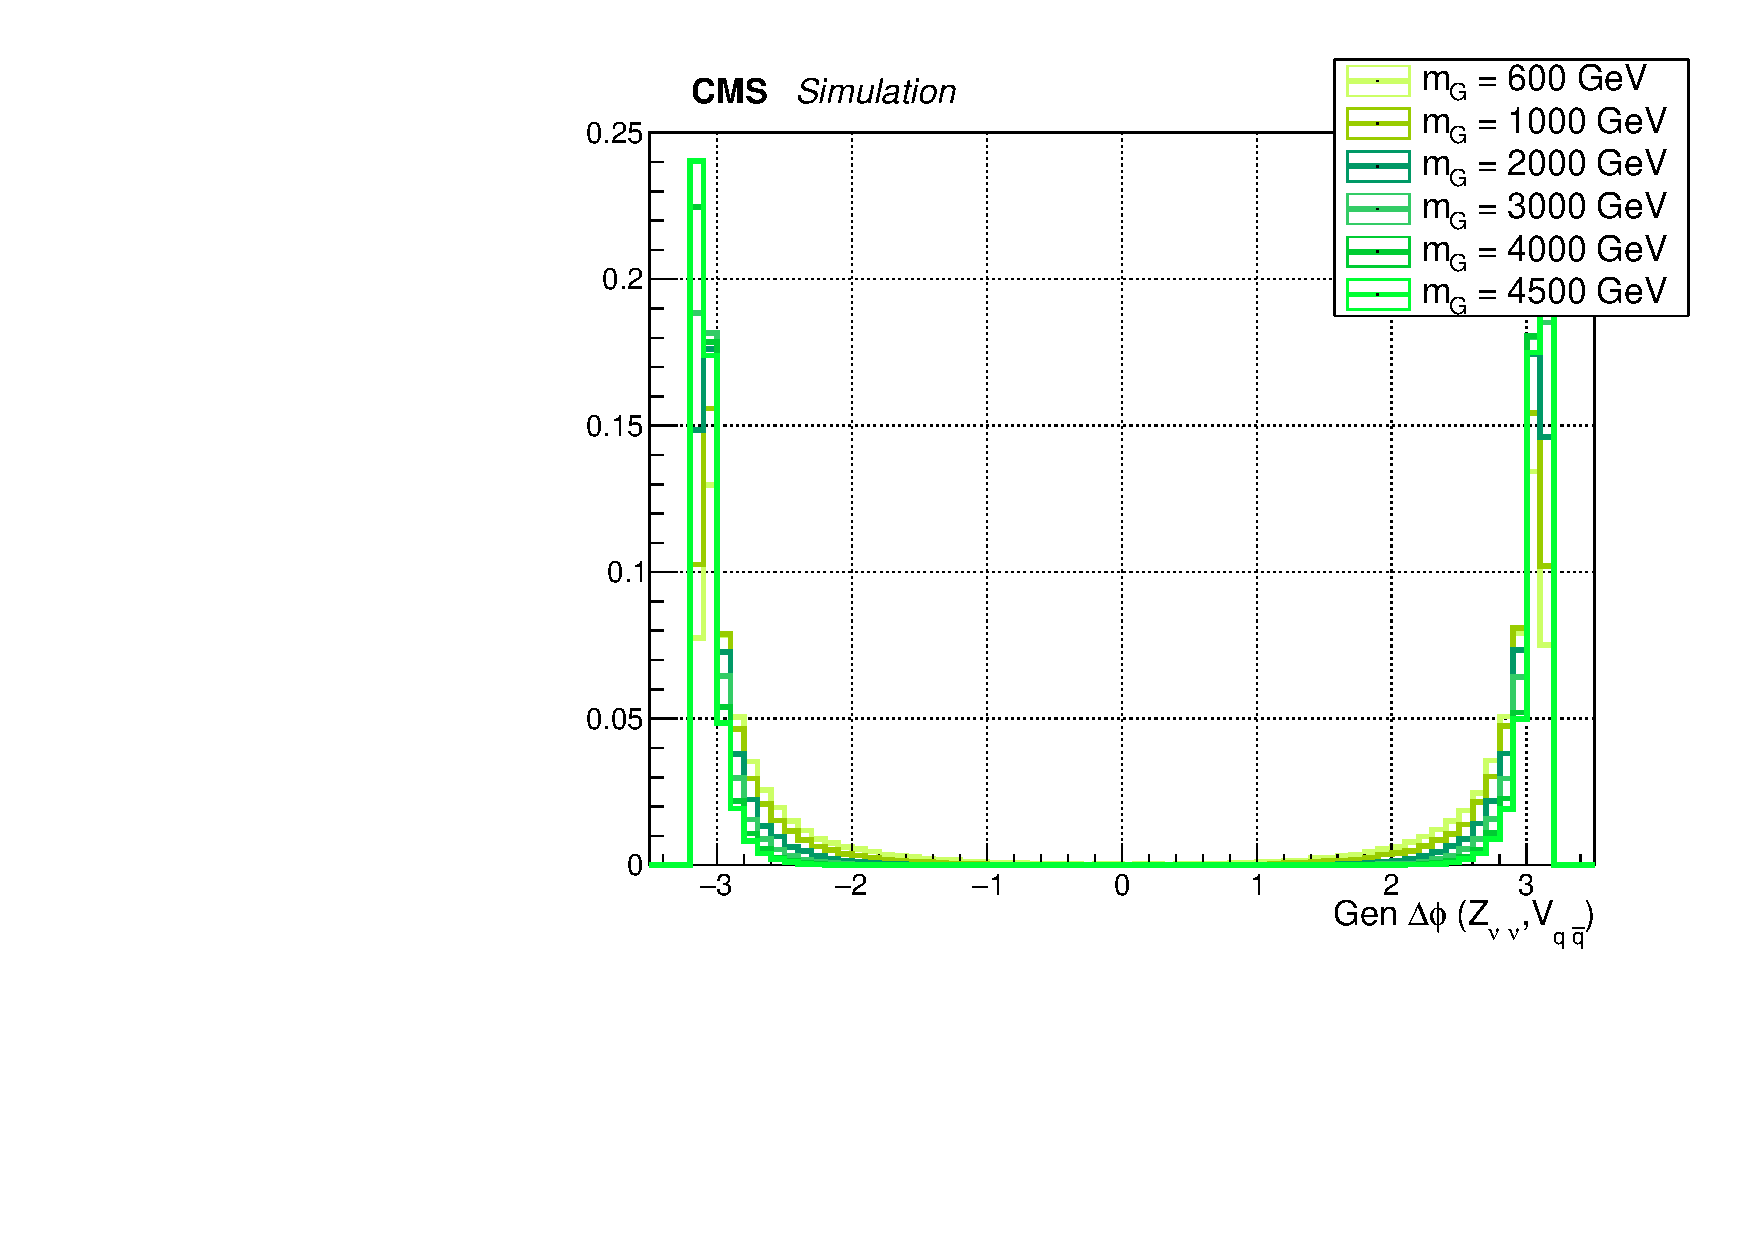
\includegraphics[width=.495\textwidth]{Gen_v9/XZZInv_g_VZDPhi.pdf}%GenPhi1pt.pdf}
     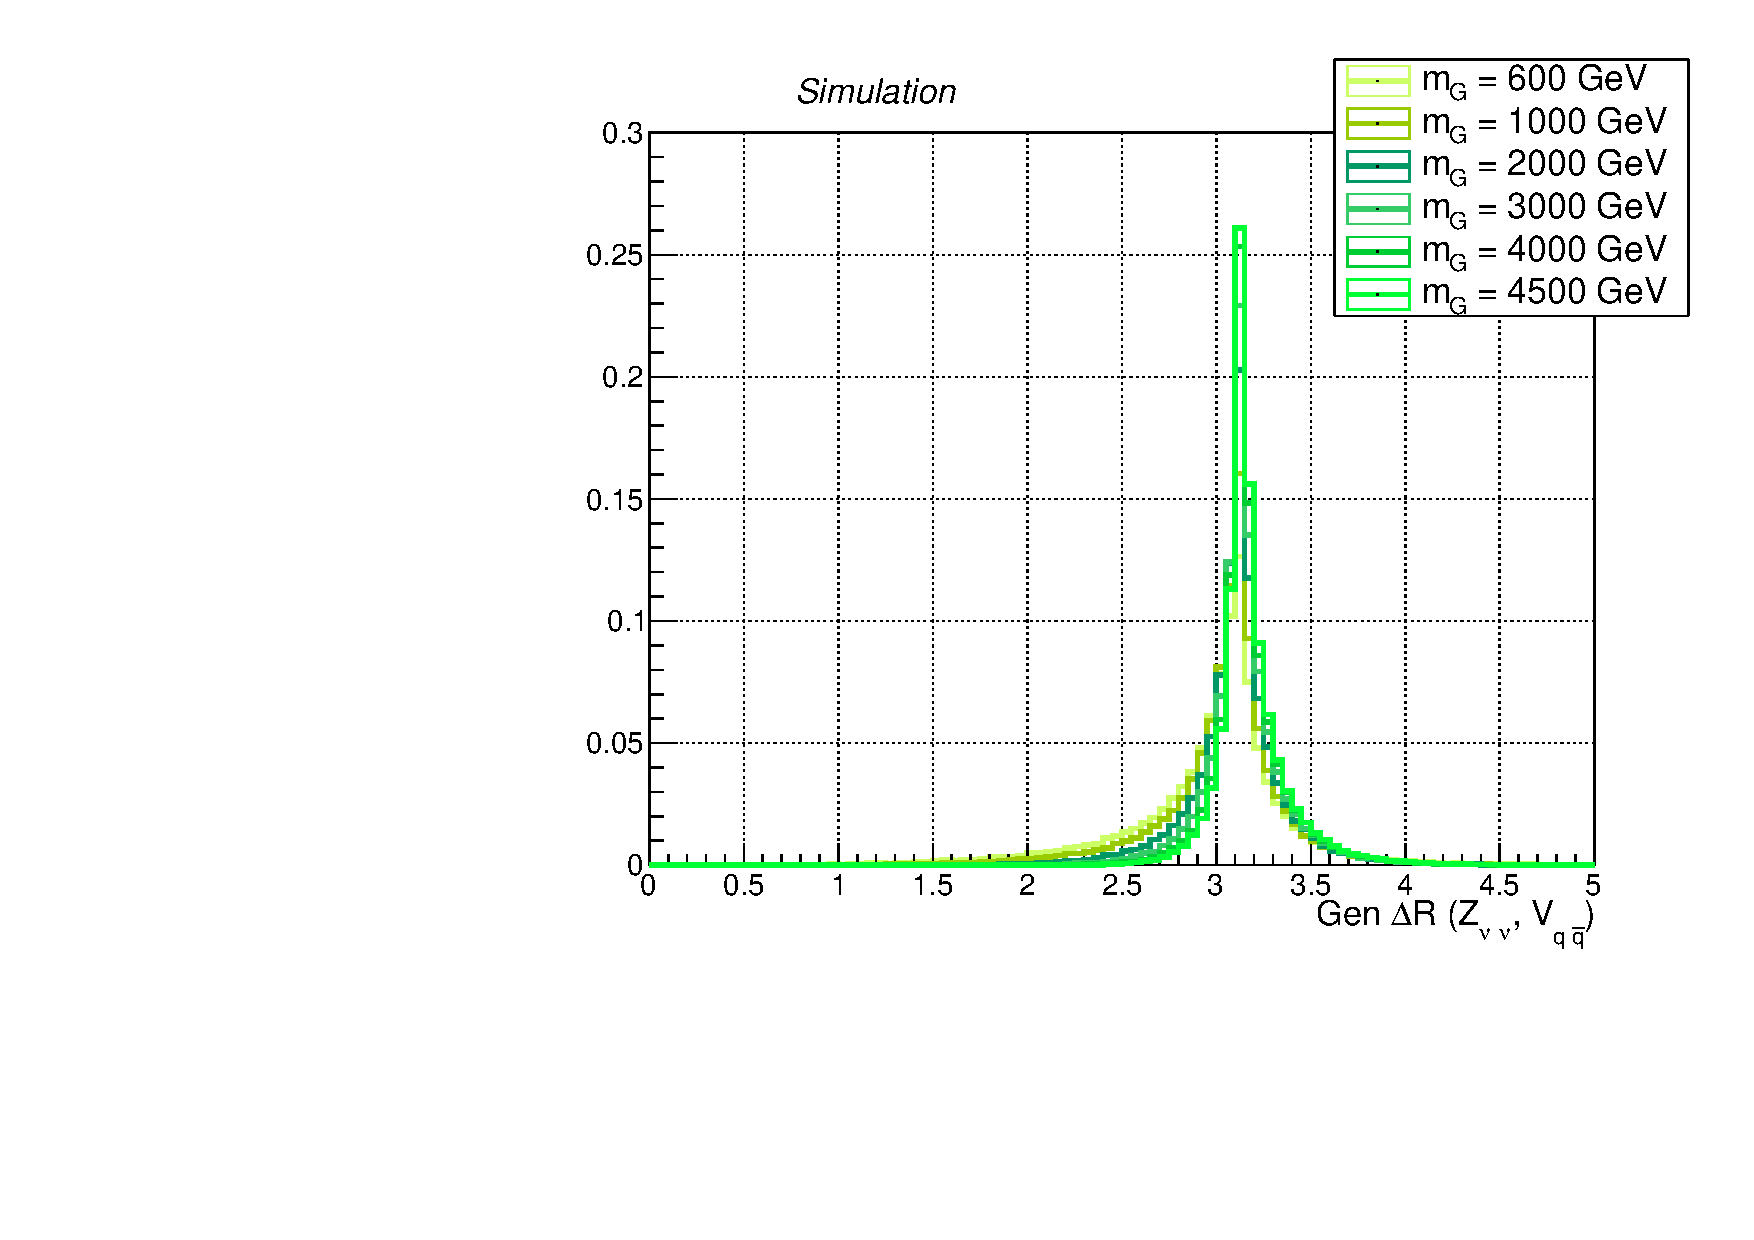
\includegraphics[width=.495\textwidth]{Gen_v9/XZZInv_g_VZDR.pdf}%GenPhi1y.pdf}
     %\\
     %\includegraphics[width=.495\textwidth]{Gen_v7/g_ZLepMass.pdf}%GenZmass.pdf}
     %\includegraphics[width=.495\textwidth]{Gen_v7/g_ZHadMass.pdf}%GenHmass.pdf}
     \\
     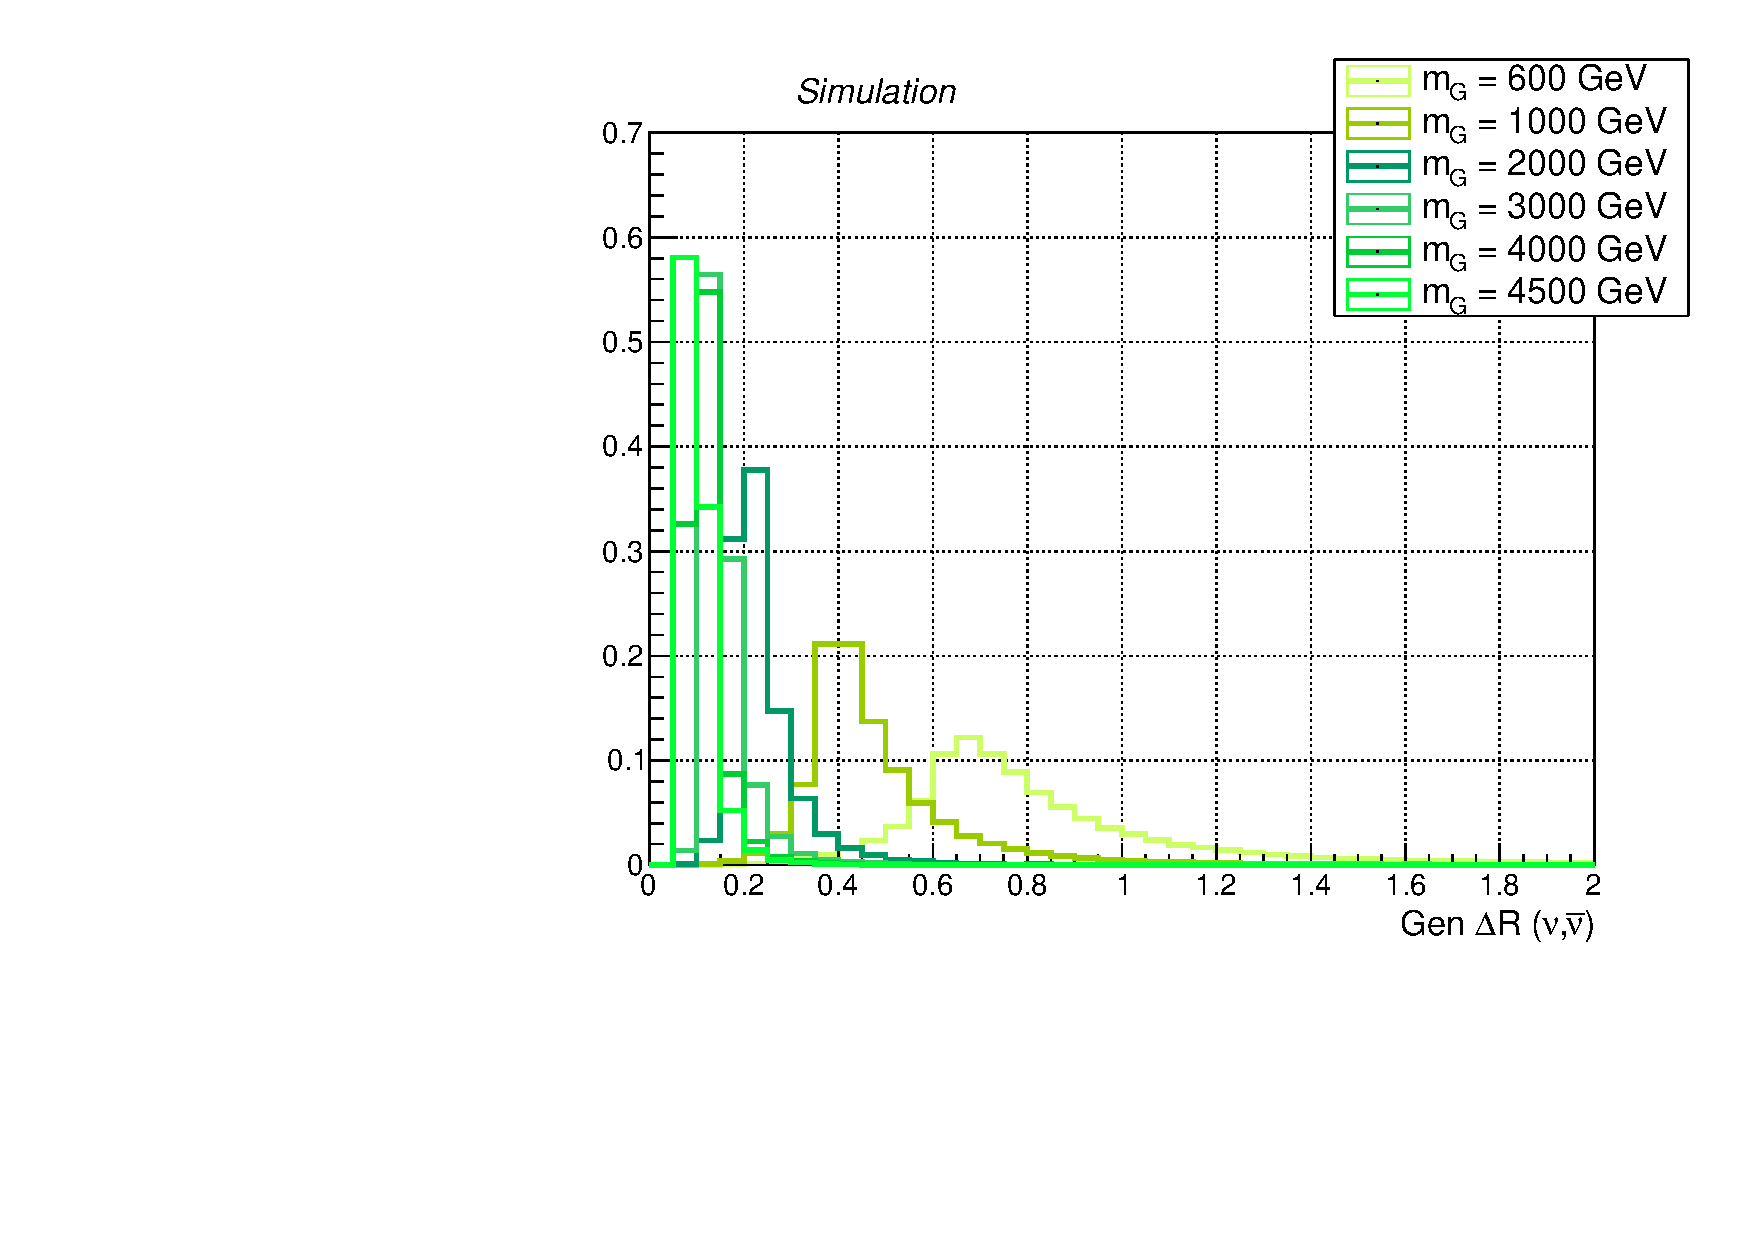
\includegraphics[width=.495\textwidth]{Gen_v9/XZZInv_g_LepDR.pdf}%GenZpt.pdf}
     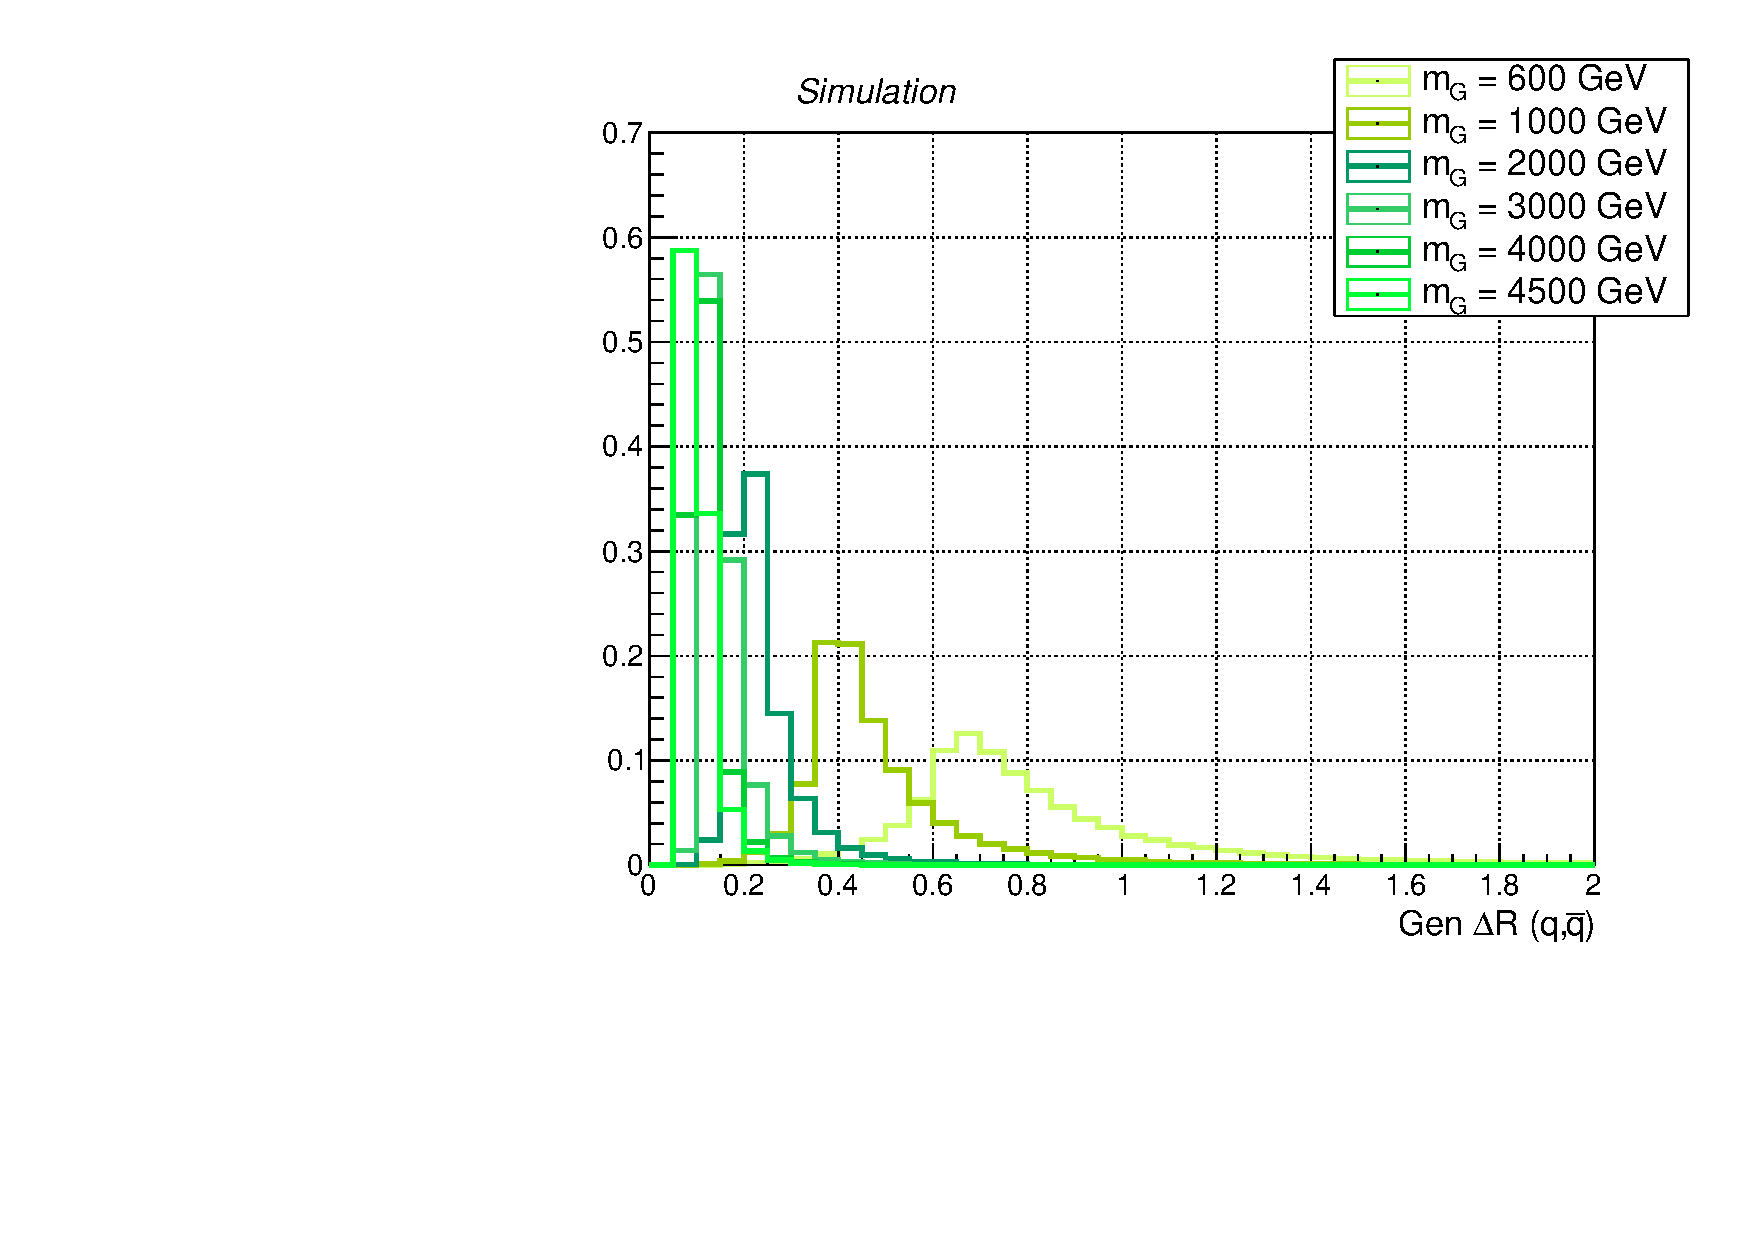
\includegraphics[width=.495\textwidth]{Gen_v9/XZZInv_g_HadDR.pdf}%GenHpt.pdf}
     \\
     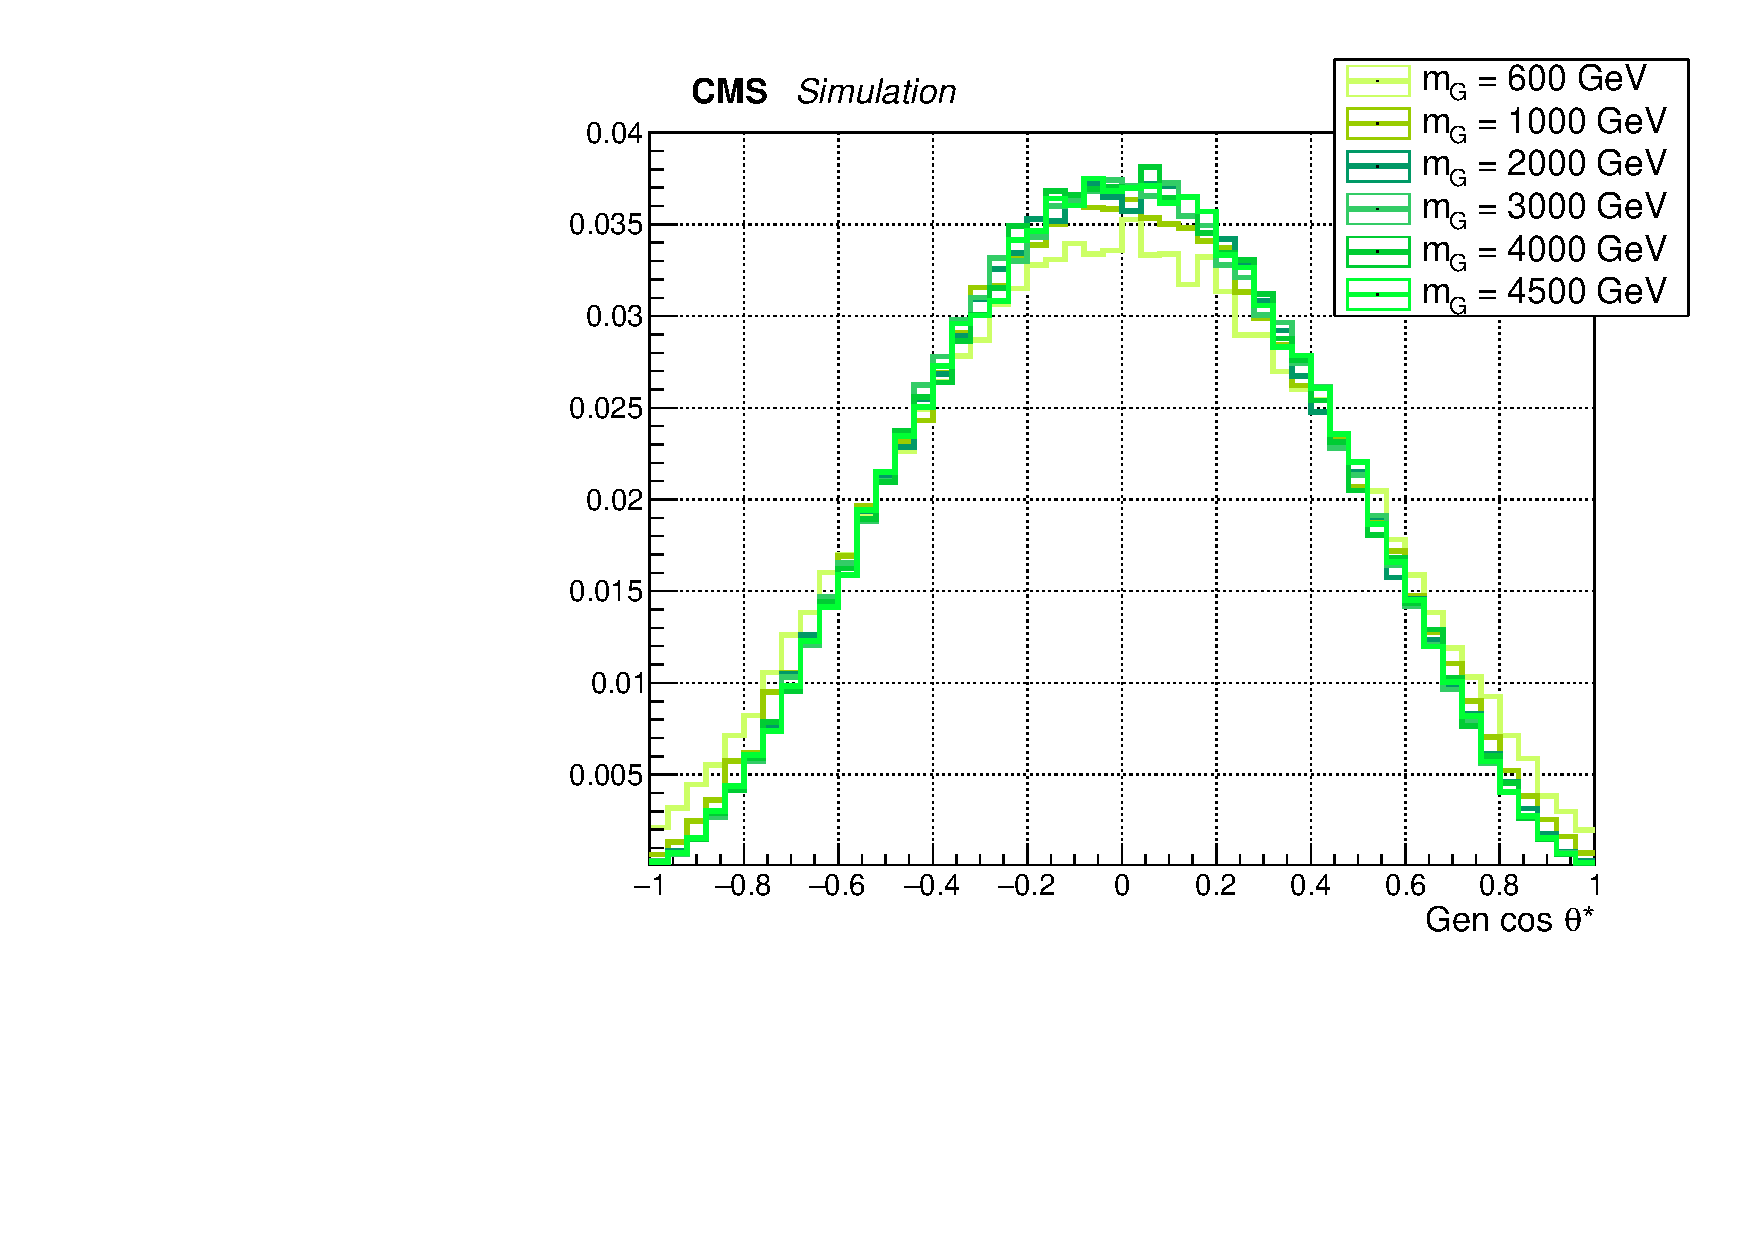
\includegraphics[width=.495\textwidth]{Gen_v9/XZZInv_g_CosThetaStar.pdf}%GenZdR.pdf}
     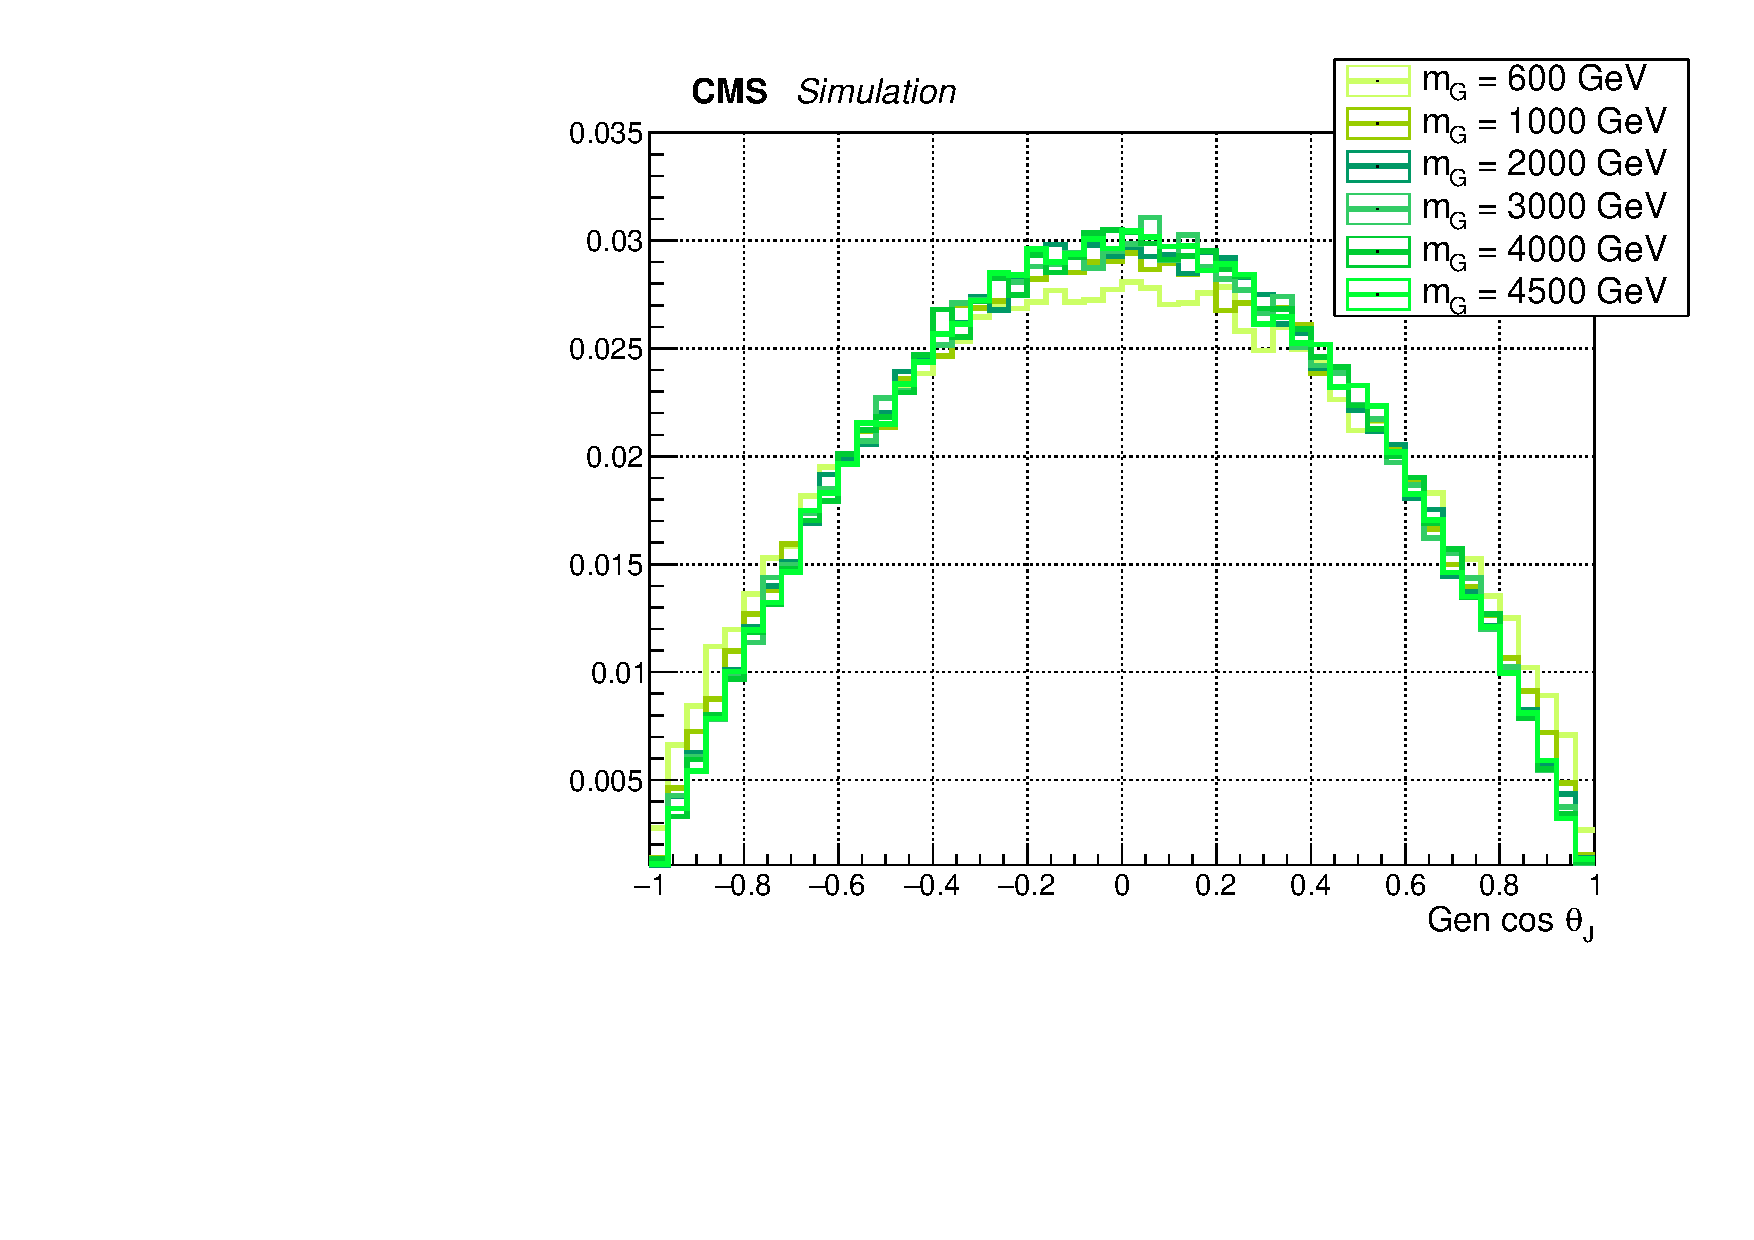
\includegraphics[width=.495\textwidth]{Gen_v9/XZZInv_g_CosThetaJ.pdf}%GenHdR.pdf}
   \end{center}
   \caption{Main signal kinematic quantities at generation level after parton showering, for spin-2 bulk graviton signal, considering different mass hypoteses ($m_{\G} = 0.6, 1, 2, 3, 4, 4.5$ TeV). Top: angular separation in the transverse plane $\Delta \varphi$ (left) and the angle $\Delta R$ (right) between leptonic \Z and hadronic \Z. Center: the angle between the neutrinos and the quarks. Bottom: distribution of $\cos{\theta}^{*}$ and $\cos{\theta}_{J}$ (described in text).}
   \label{fig:genGravSignal3}
 \end{figure}

 \begin{figure}[!htb]
   \begin{center}
     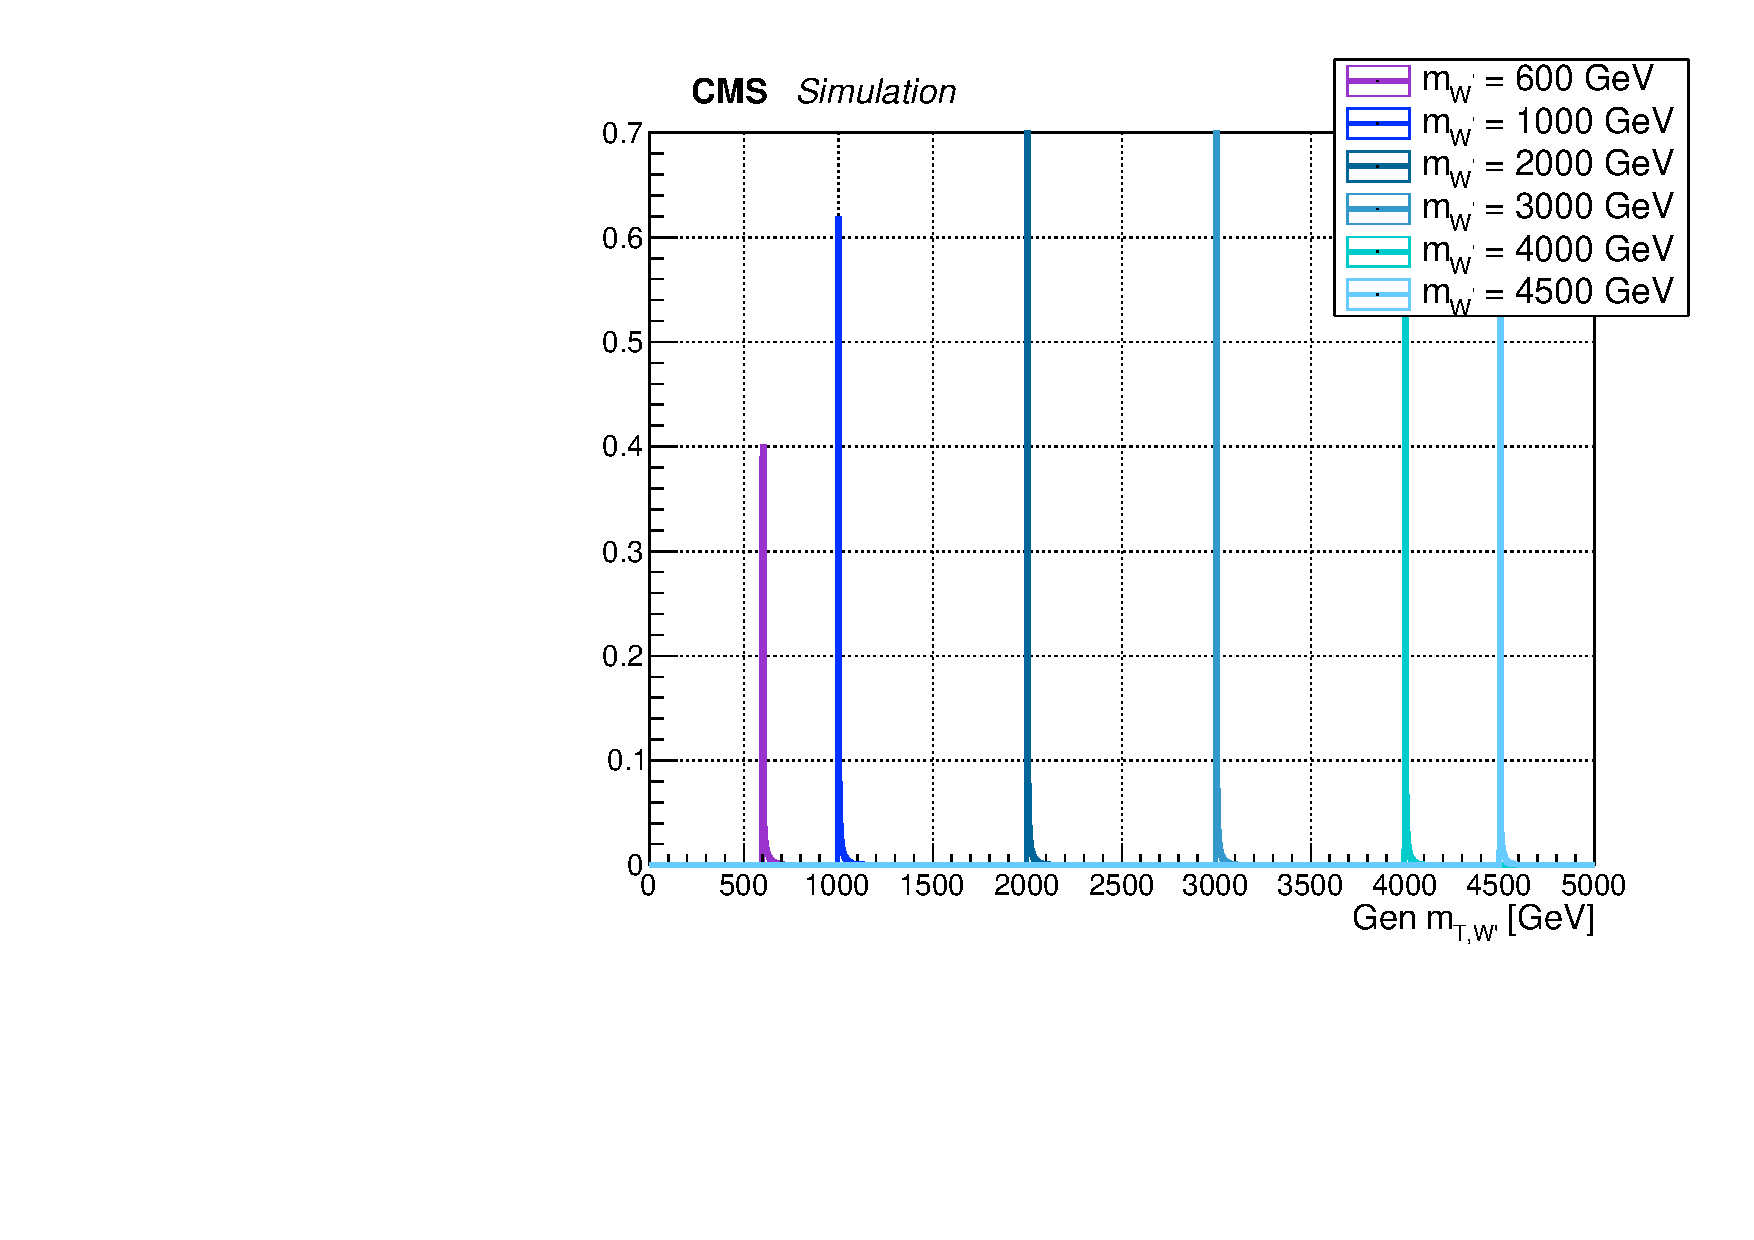
\includegraphics[width=.495\textwidth]{Gen_v9/XWZInv_g_XMT.pdf}%GenPhi1pt.pdf}
     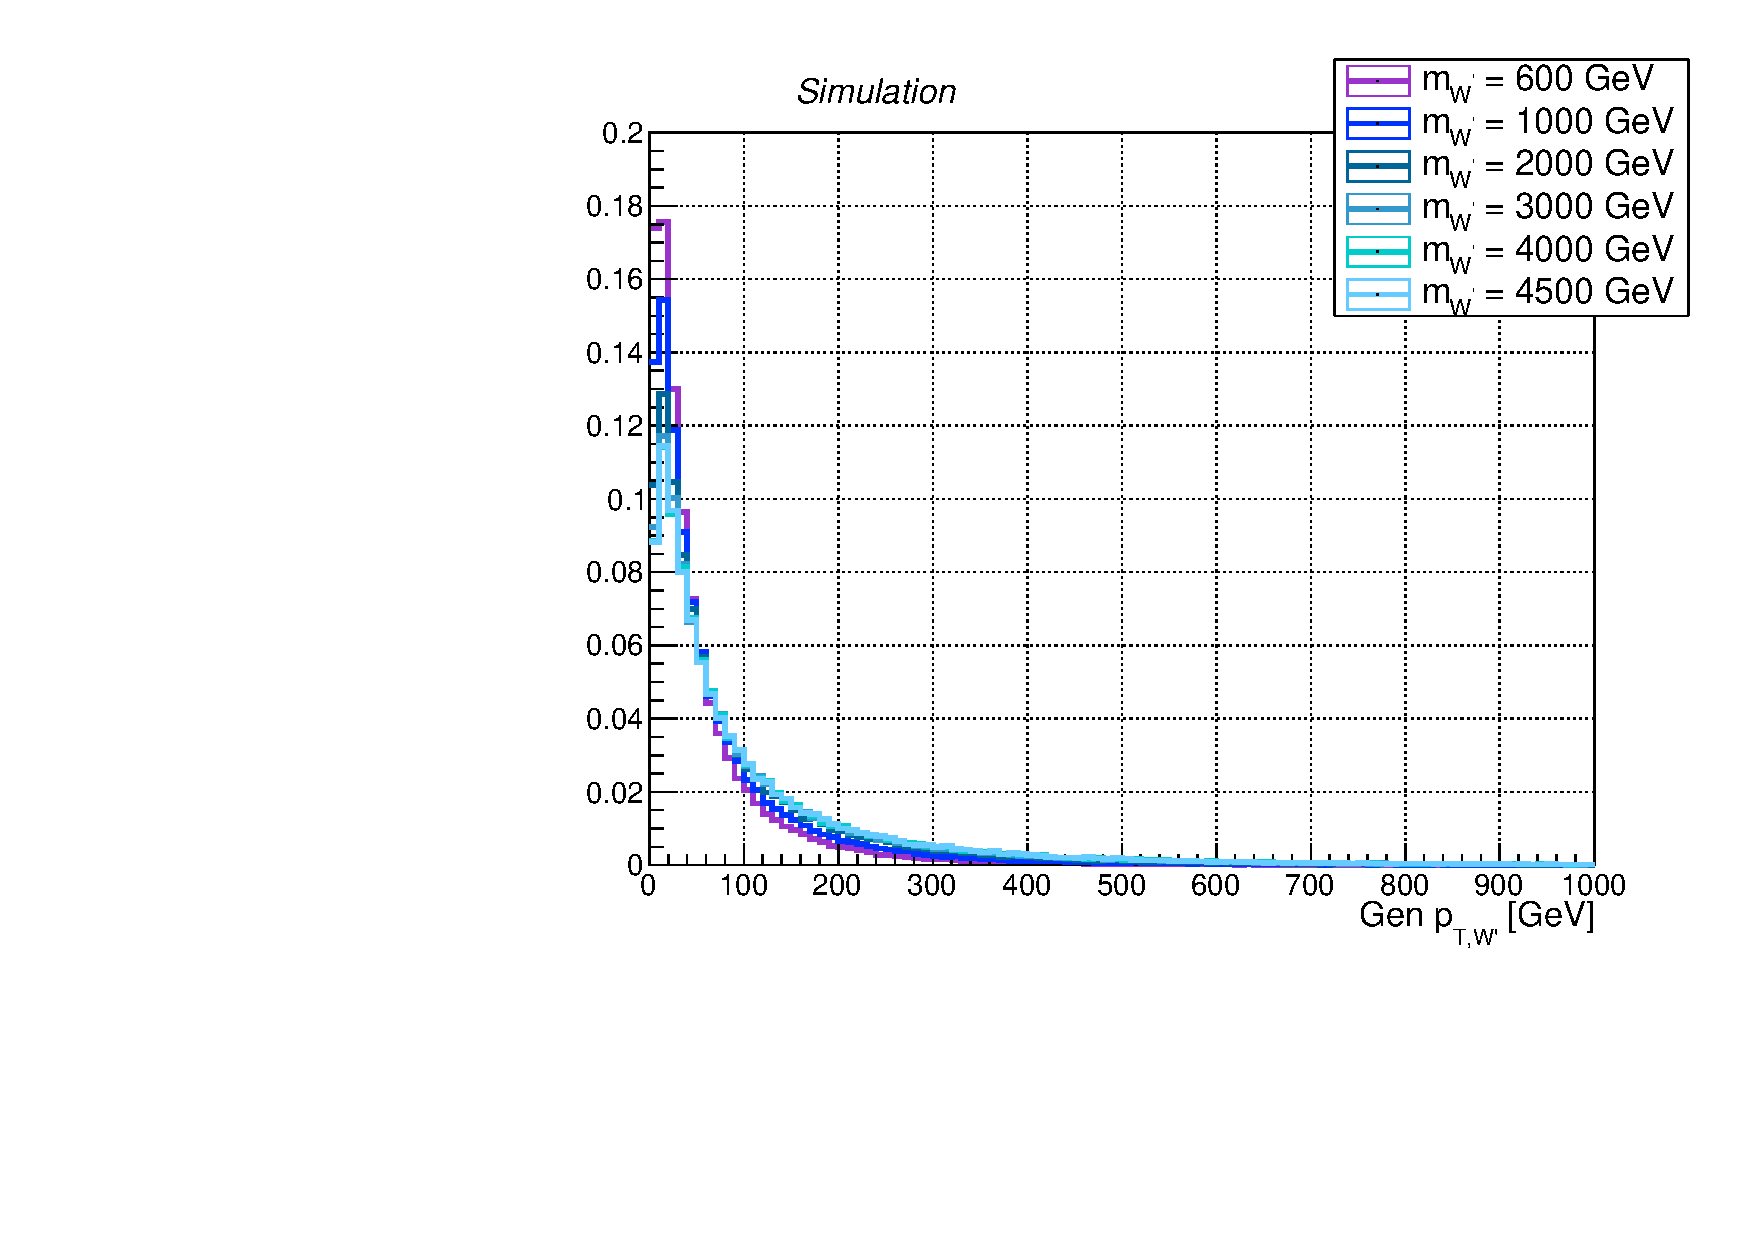
\includegraphics[width=.495\textwidth]{Gen_v9/XWZInv_g_XPt.pdf}%GenPhi1y.pdf}
     %\\
     %\includegraphics[width=.495\textwidth]{Gen_v7/g_ZLepMass.pdf}%GenZmass.pdf}
     %\includegraphics[width=.495\textwidth]{Gen_v7/g_ZHadMass.pdf}%GenHmass.pdf}
     \\
     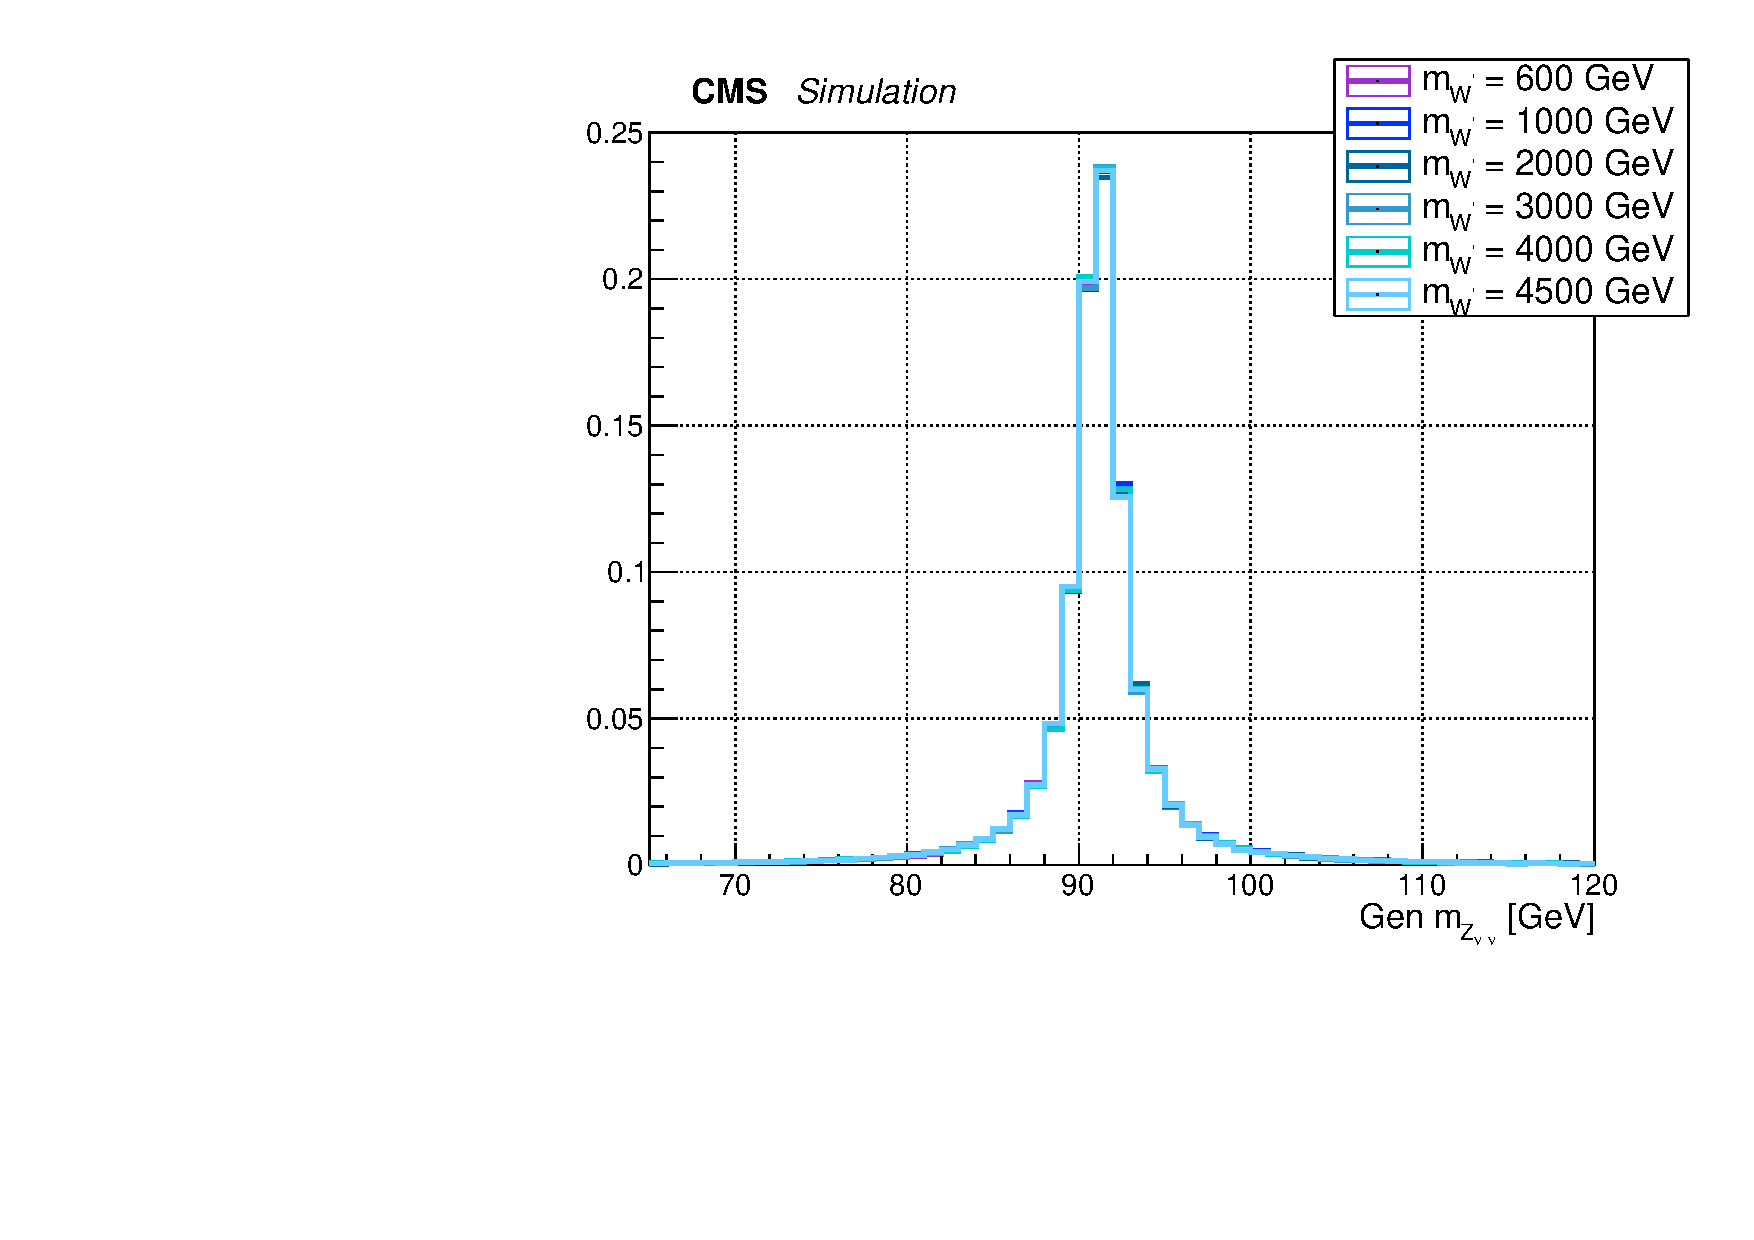
\includegraphics[width=.495\textwidth]{Gen_v9/XWZInv_g_ZLepMass.pdf}%GenZpt.pdf}
     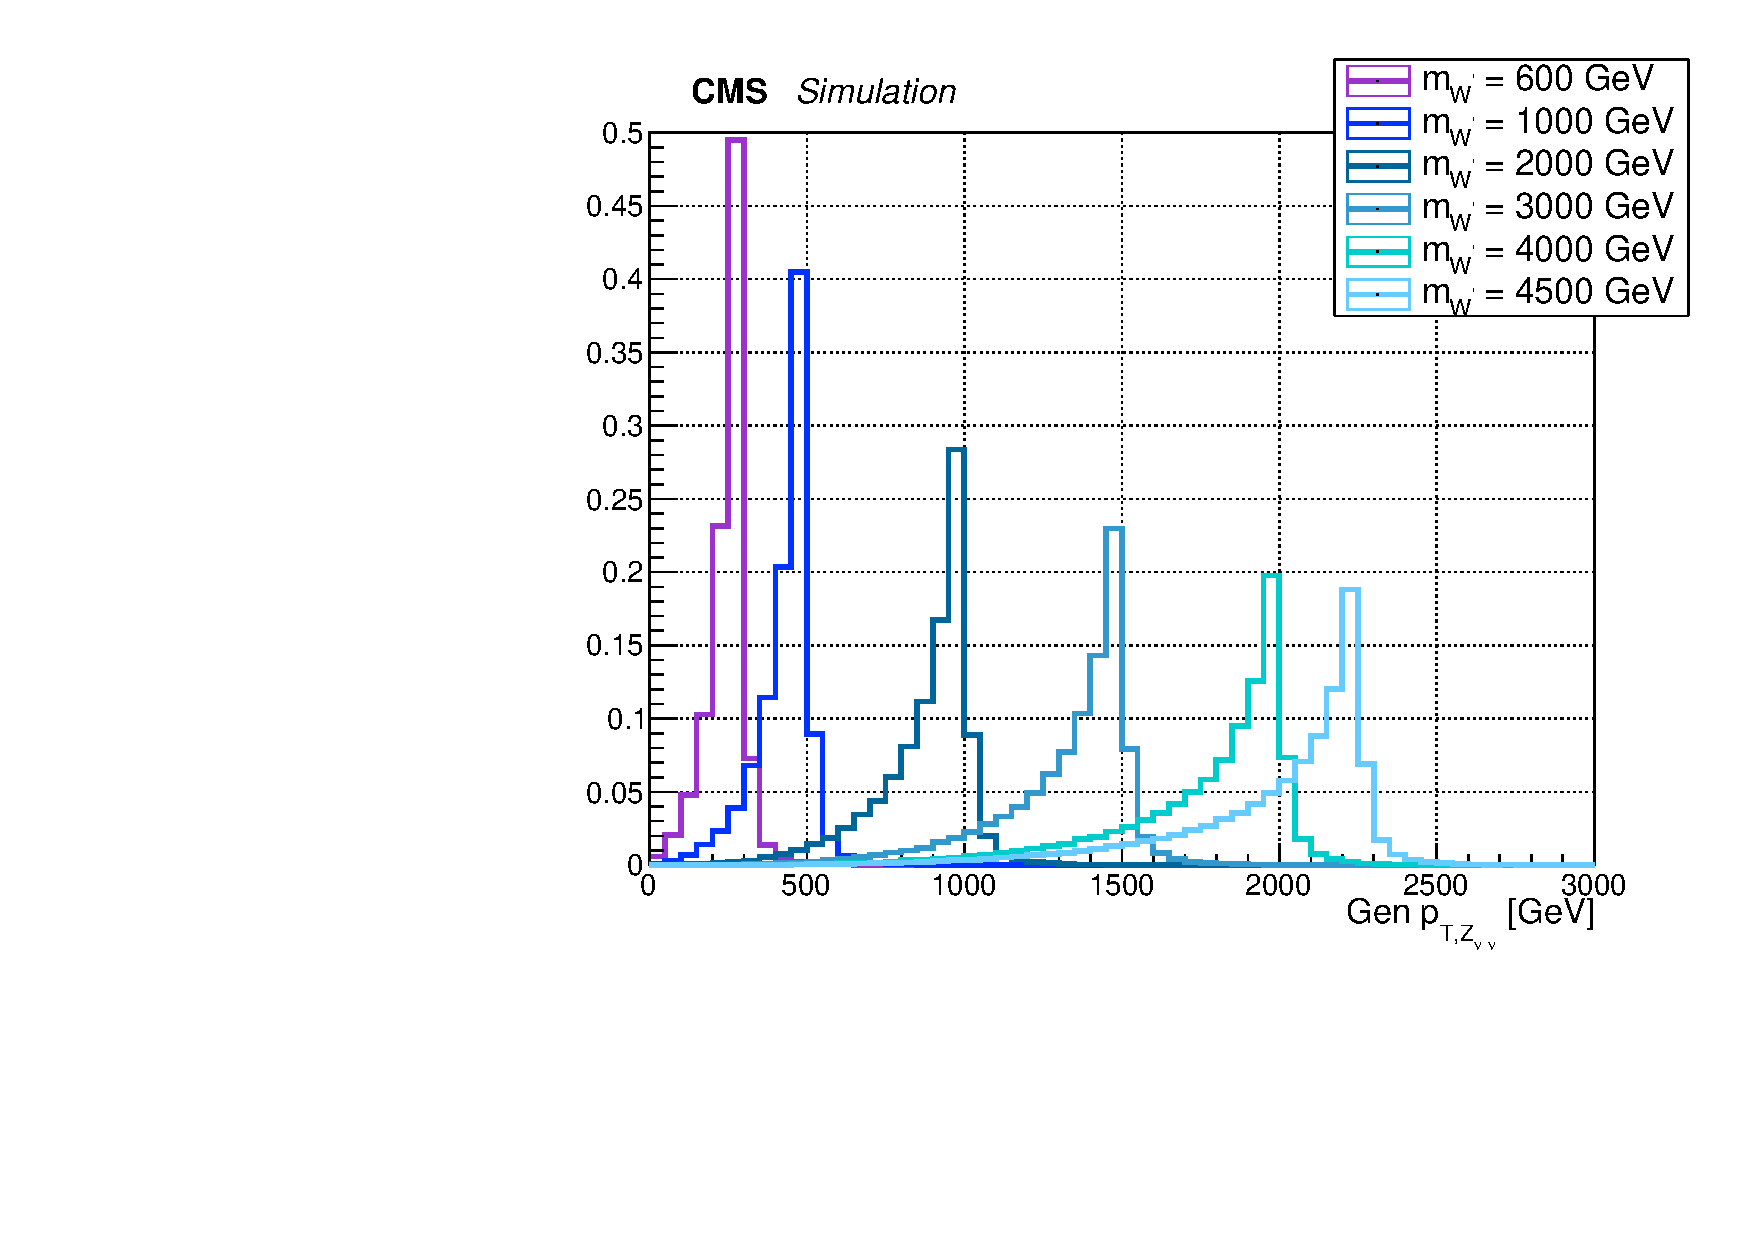
\includegraphics[width=.495\textwidth]{Gen_v9/XWZInv_g_ZLepPt.pdf}%GenHpt.pdf}
     \\
     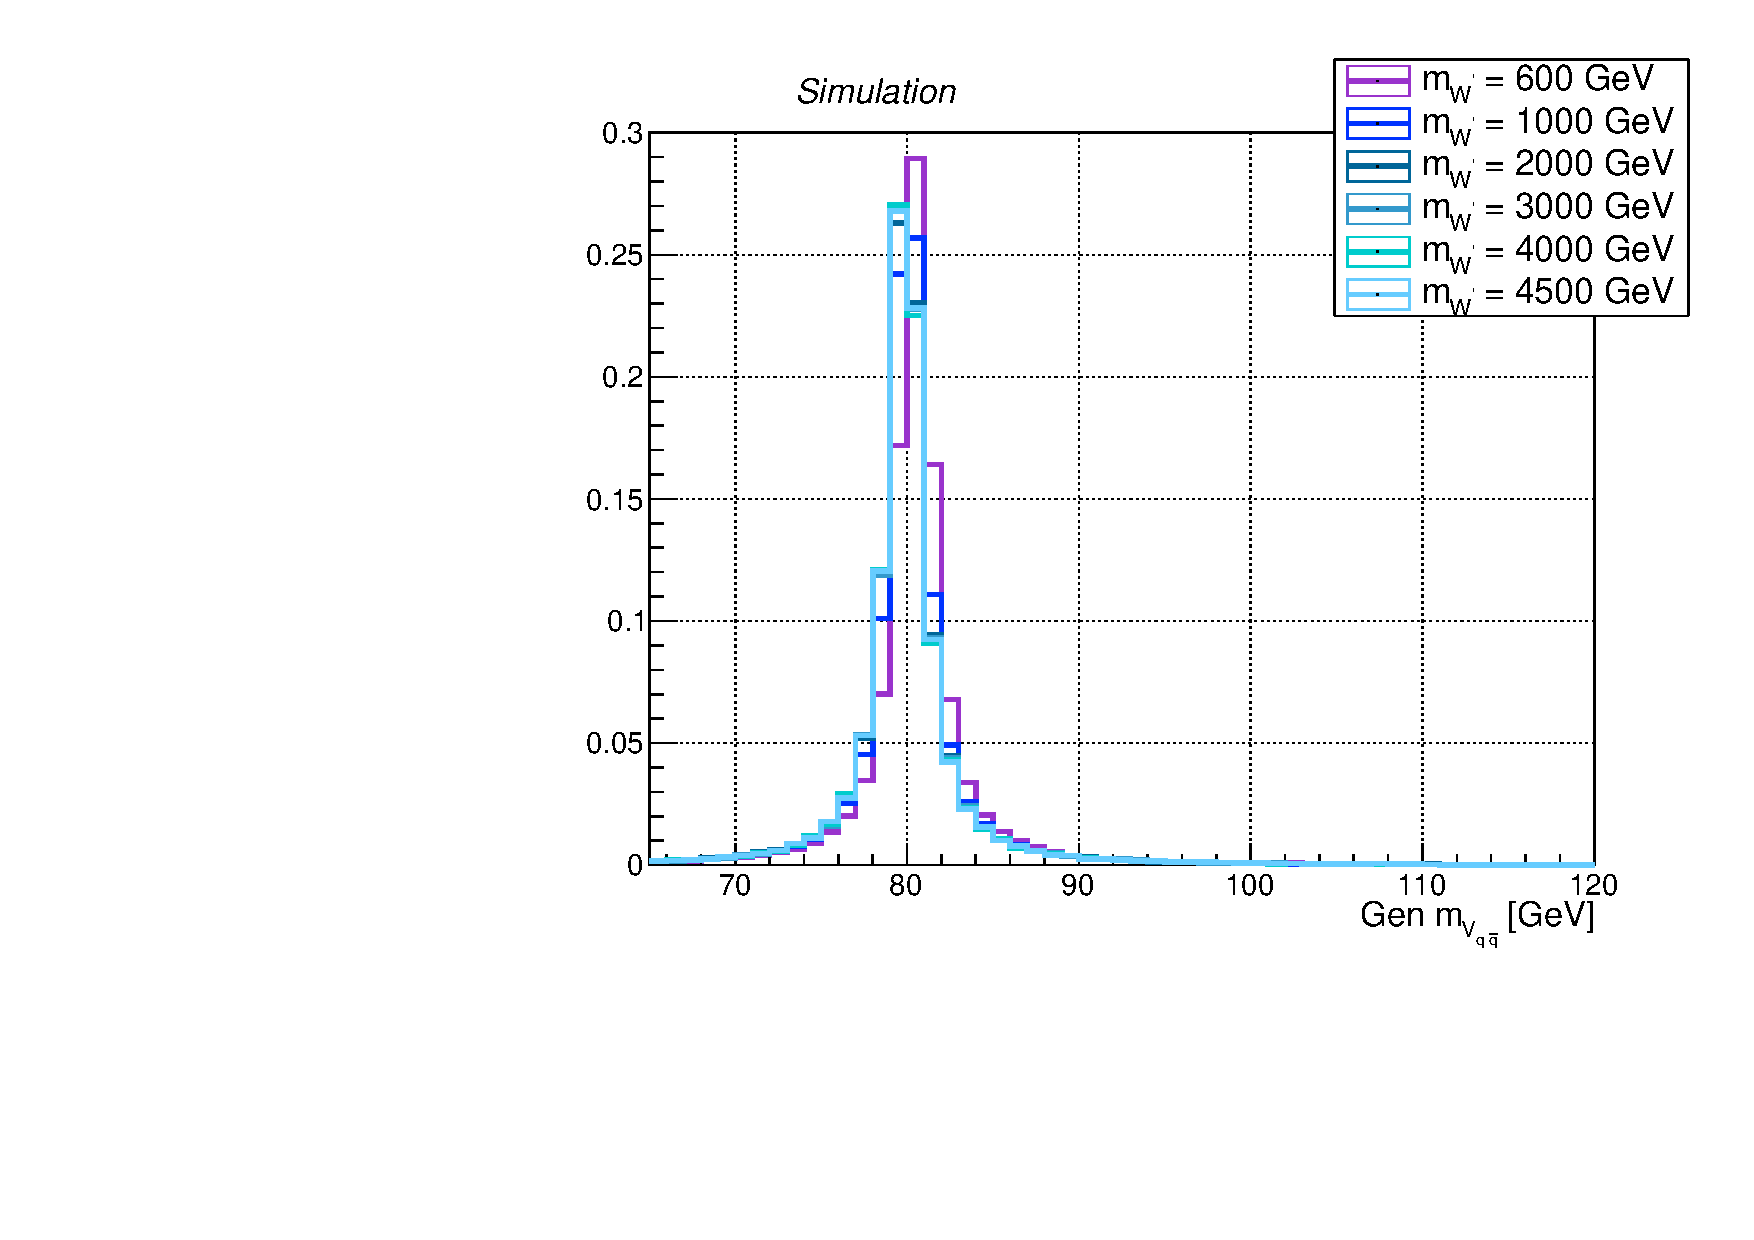
\includegraphics[width=.495\textwidth]{Gen_v9/XWZInv_g_VHadMass.pdf}%GenZdR.pdf}
     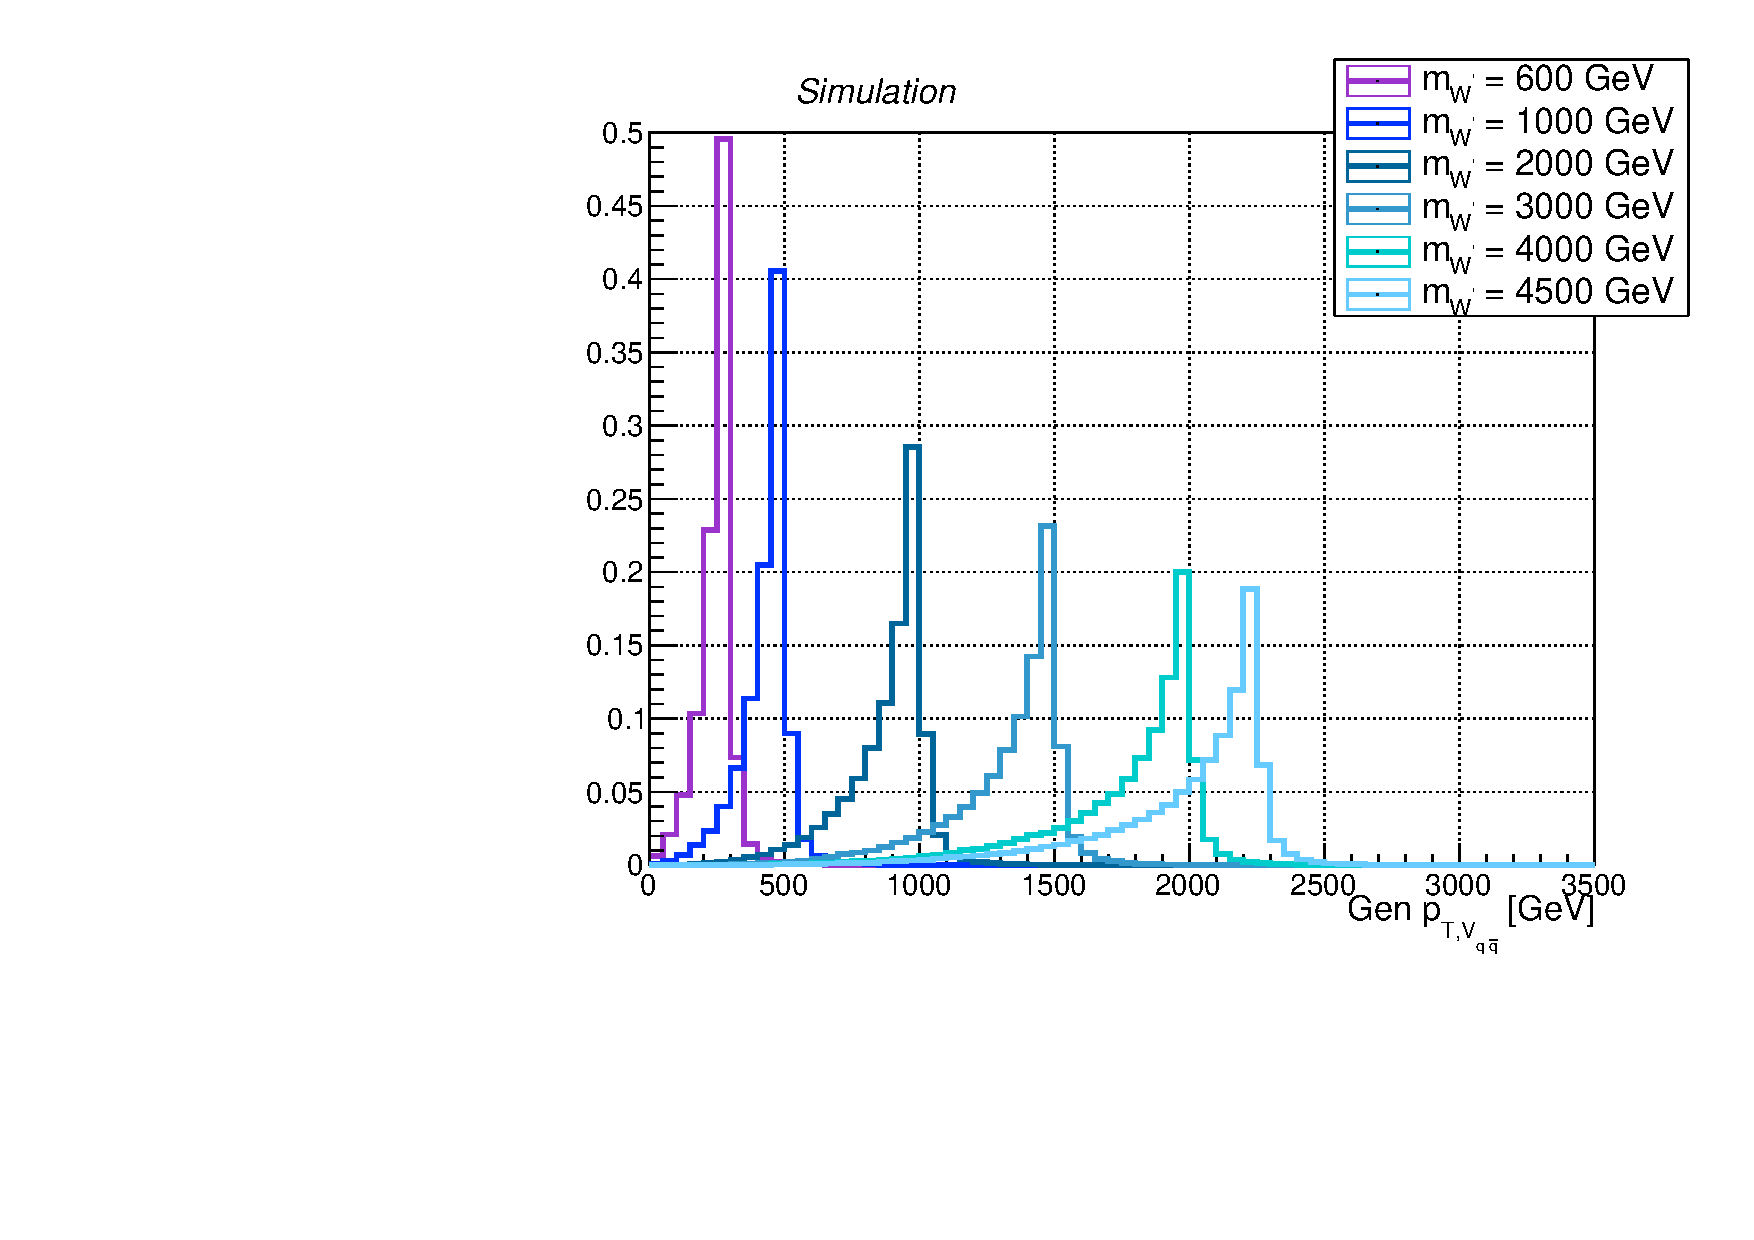
\includegraphics[width=.495\textwidth]{Gen_v9/XWZInv_g_VHadPt.pdf}%GenHdR.pdf}
   \end{center}
   \caption{Main signal kinematic quantities at generation level after parton showering, for spin-1 \Wp signal, considering different mass hypoteses ($m_{\Wp} = 0.6, 1, 2, 3, 4, 4.5$ TeV). Top: \Wp transverse mass and \pt distributions. Center: invisibly decaying \Z mass and \pt. Bottom: hadronically decaying \W mass and \pt.}
   \label{fig:genWprimeSignal1}
 \end{figure}

 \begin{figure}[!htb]
   \begin{center}
     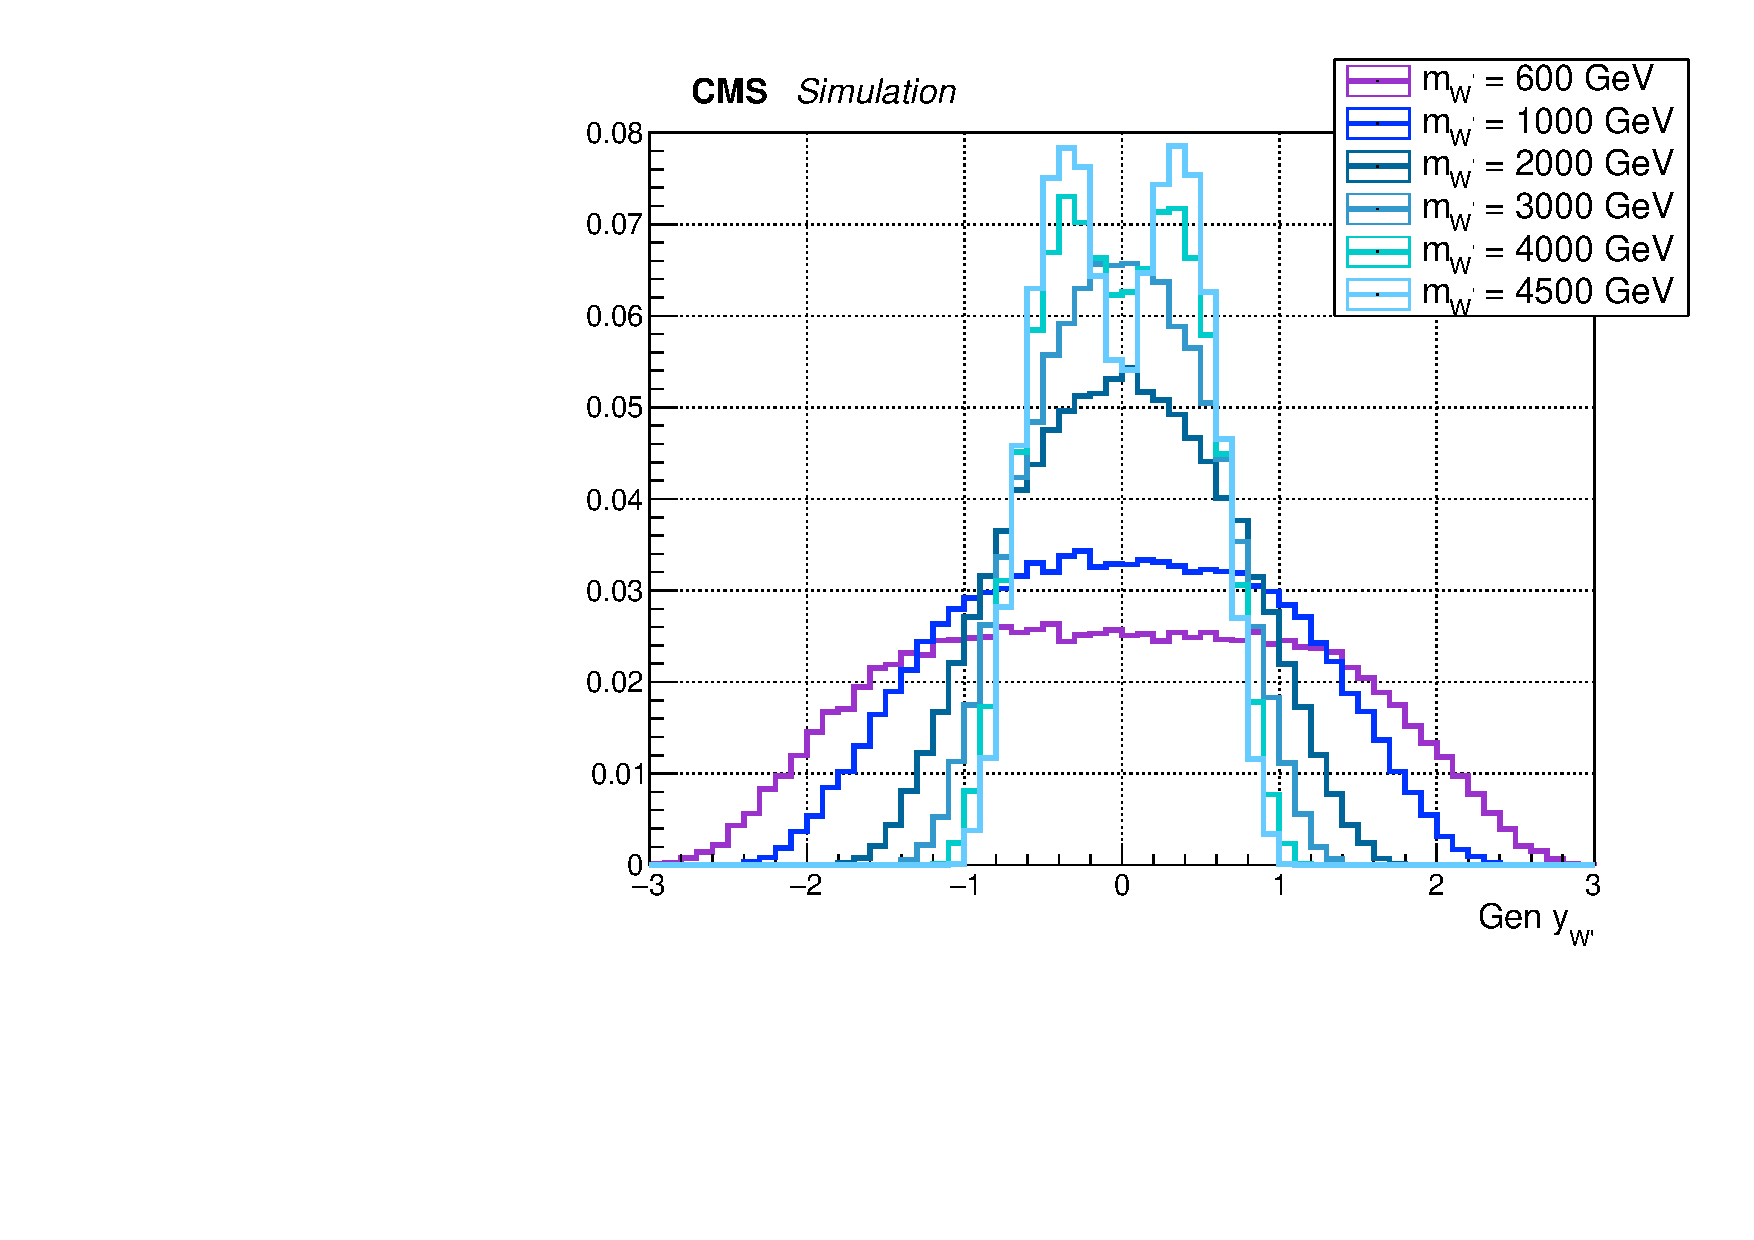
\includegraphics[width=.495\textwidth]{Gen_v9/XWZInv_g_XRapidity.pdf}%GenPhi1pt.pdf}
     %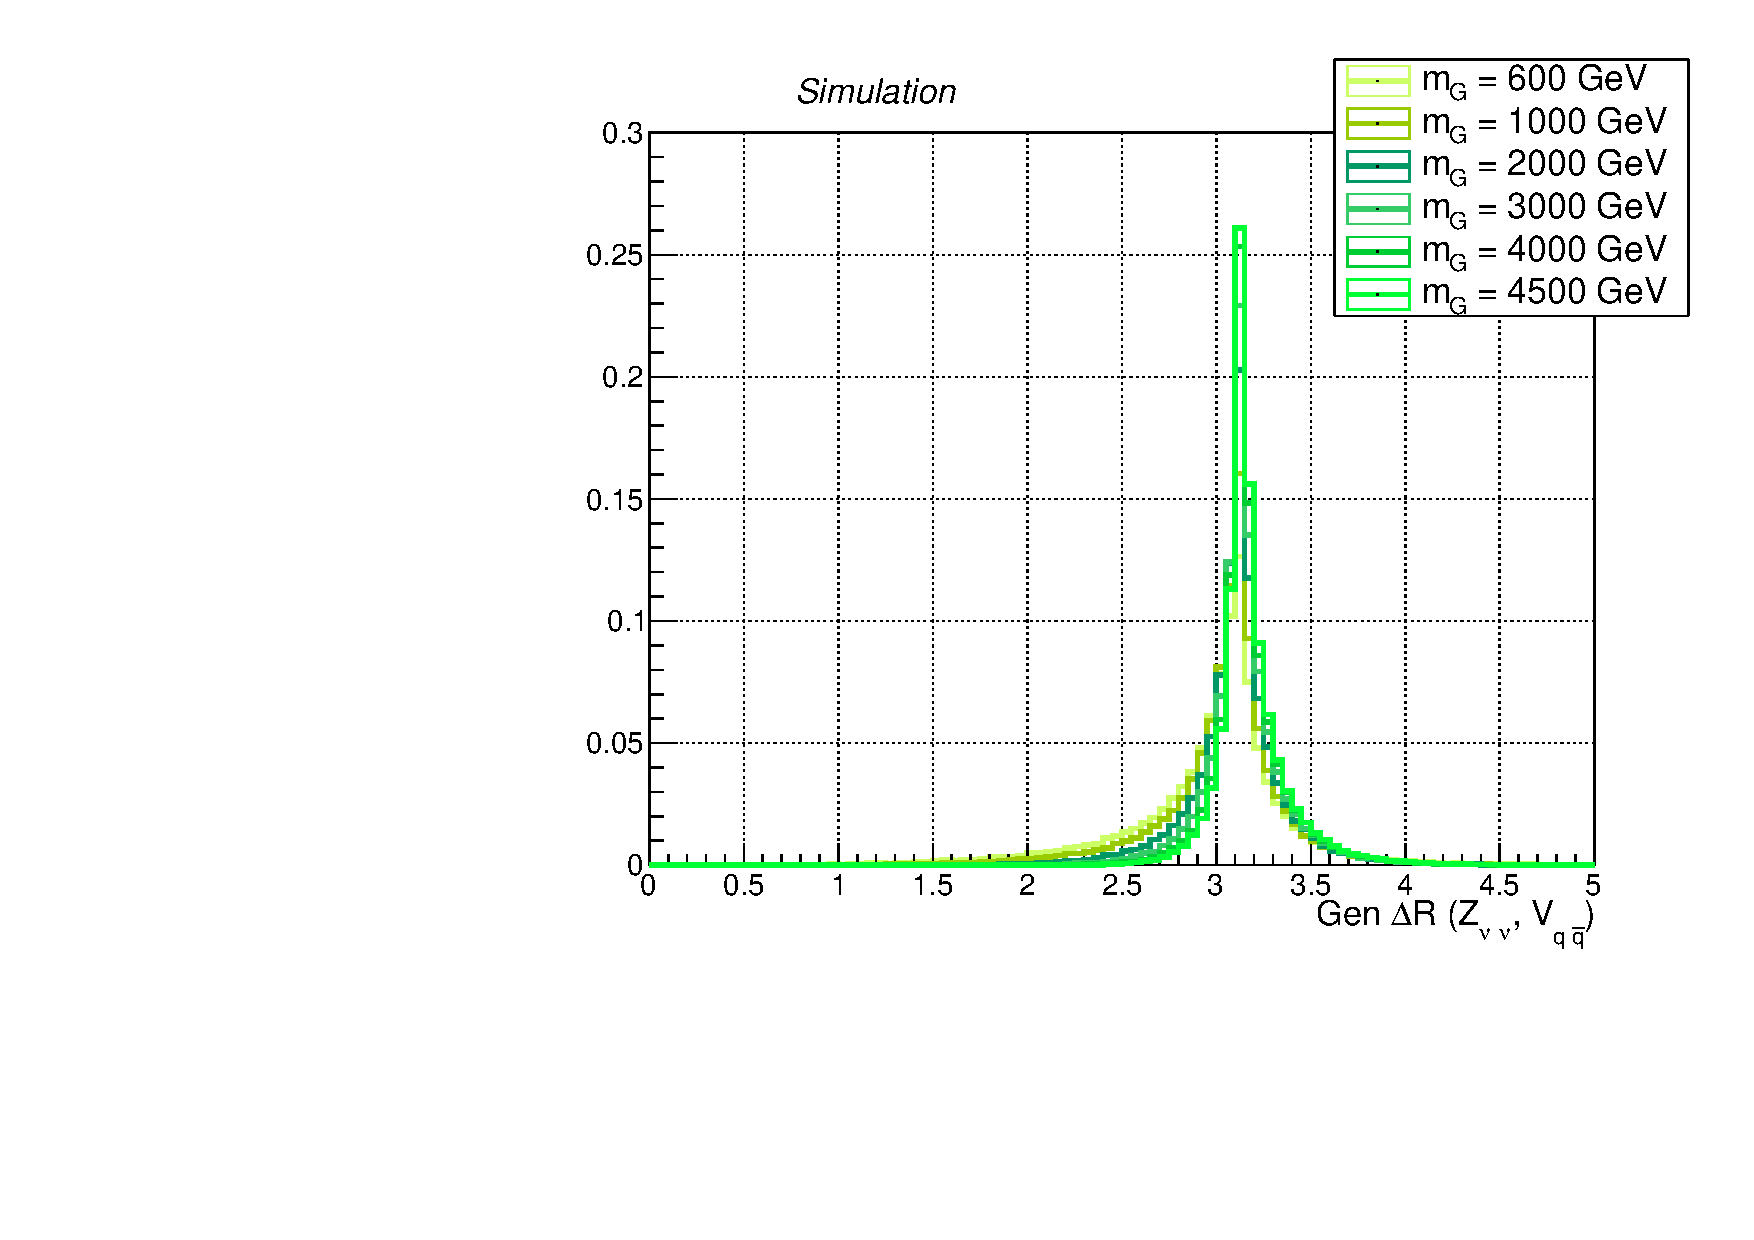
\includegraphics[width=.495\textwidth]{Gen_v9/XZZInv_g_VZDR.pdf}%GenPhi1y.pdf}
     %\\
     %\includegraphics[width=.495\textwidth]{Gen_v7/g_ZLepMass.pdf}%GenZmass.pdf}
     %\includegraphics[width=.495\textwidth]{Gen_v7/g_ZHadMass.pdf}%GenHmass.pdf}
     \\
     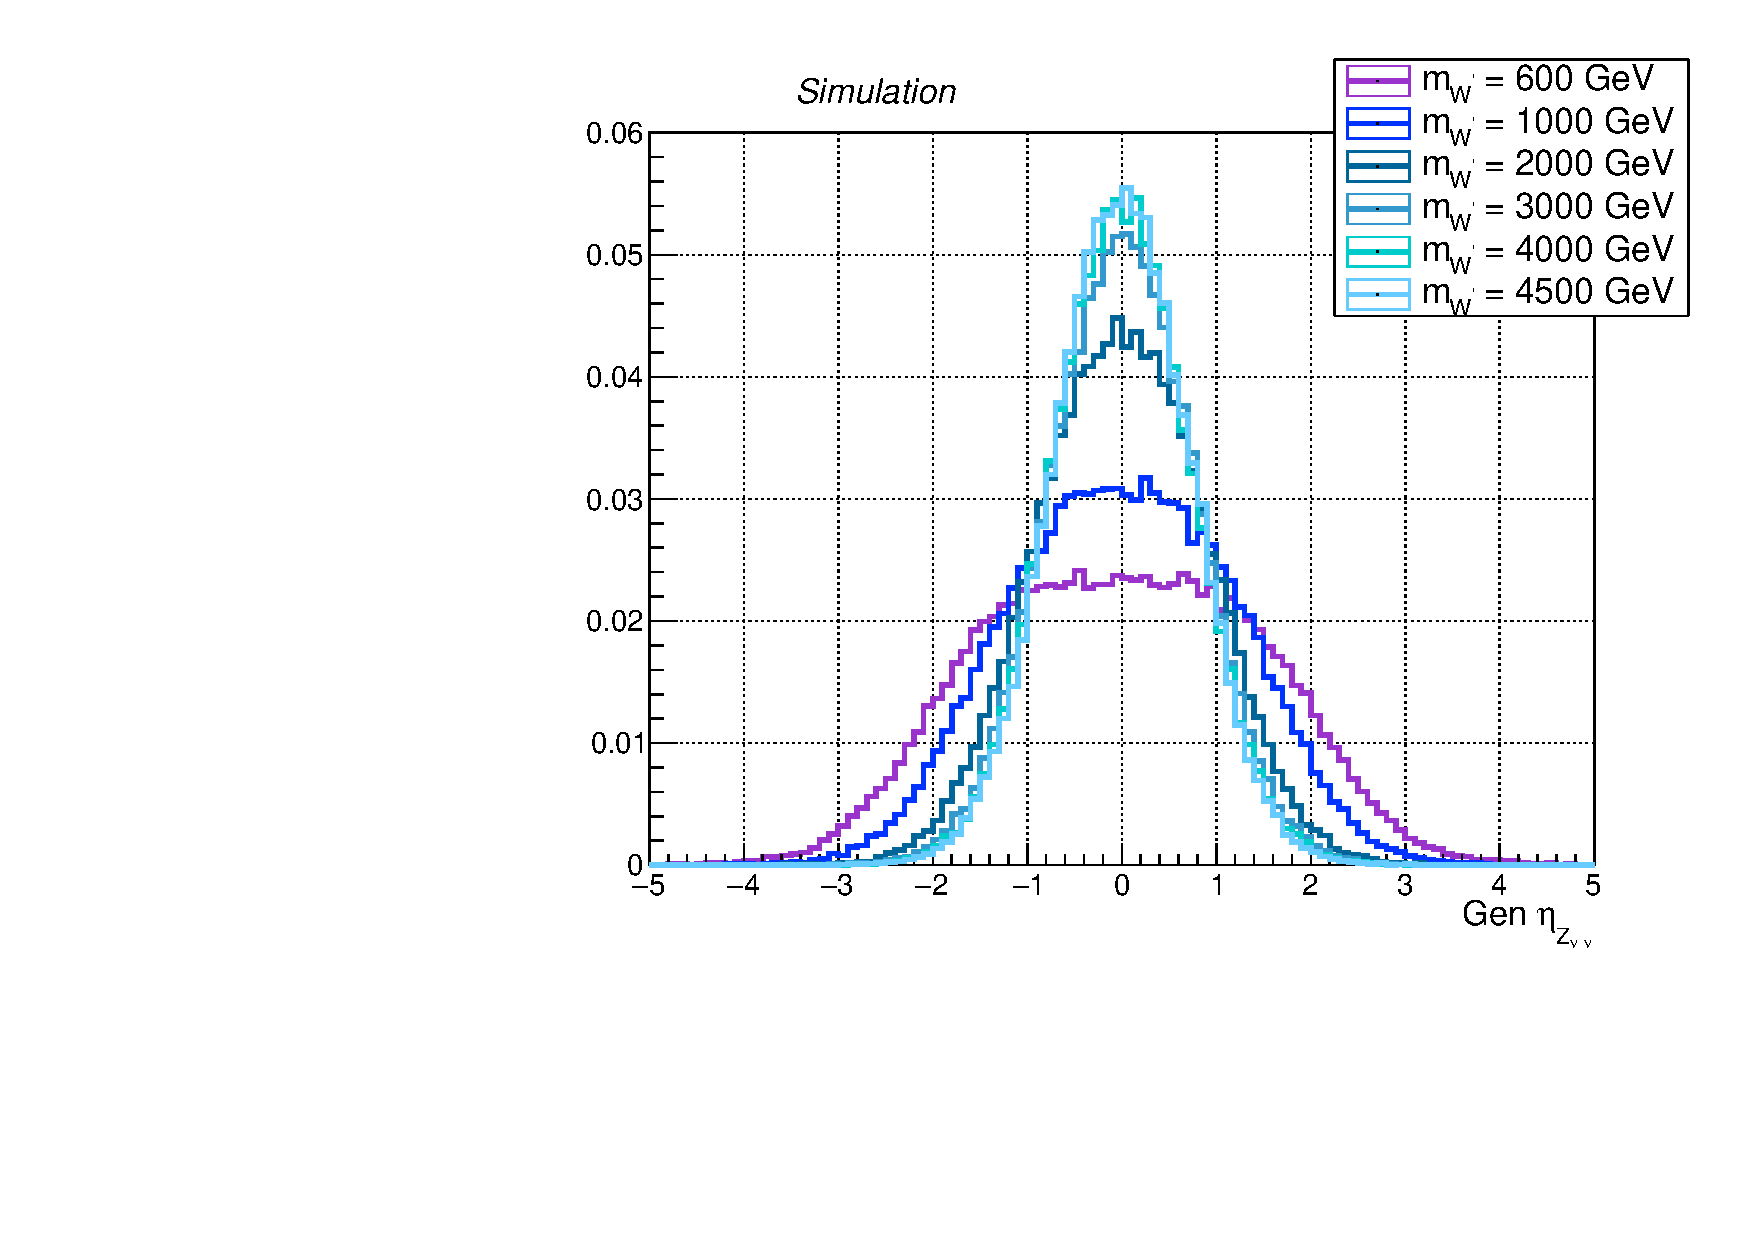
\includegraphics[width=.495\textwidth]{Gen_v9/XWZInv_g_ZLepEta.pdf}%GenZpt.pdf}
     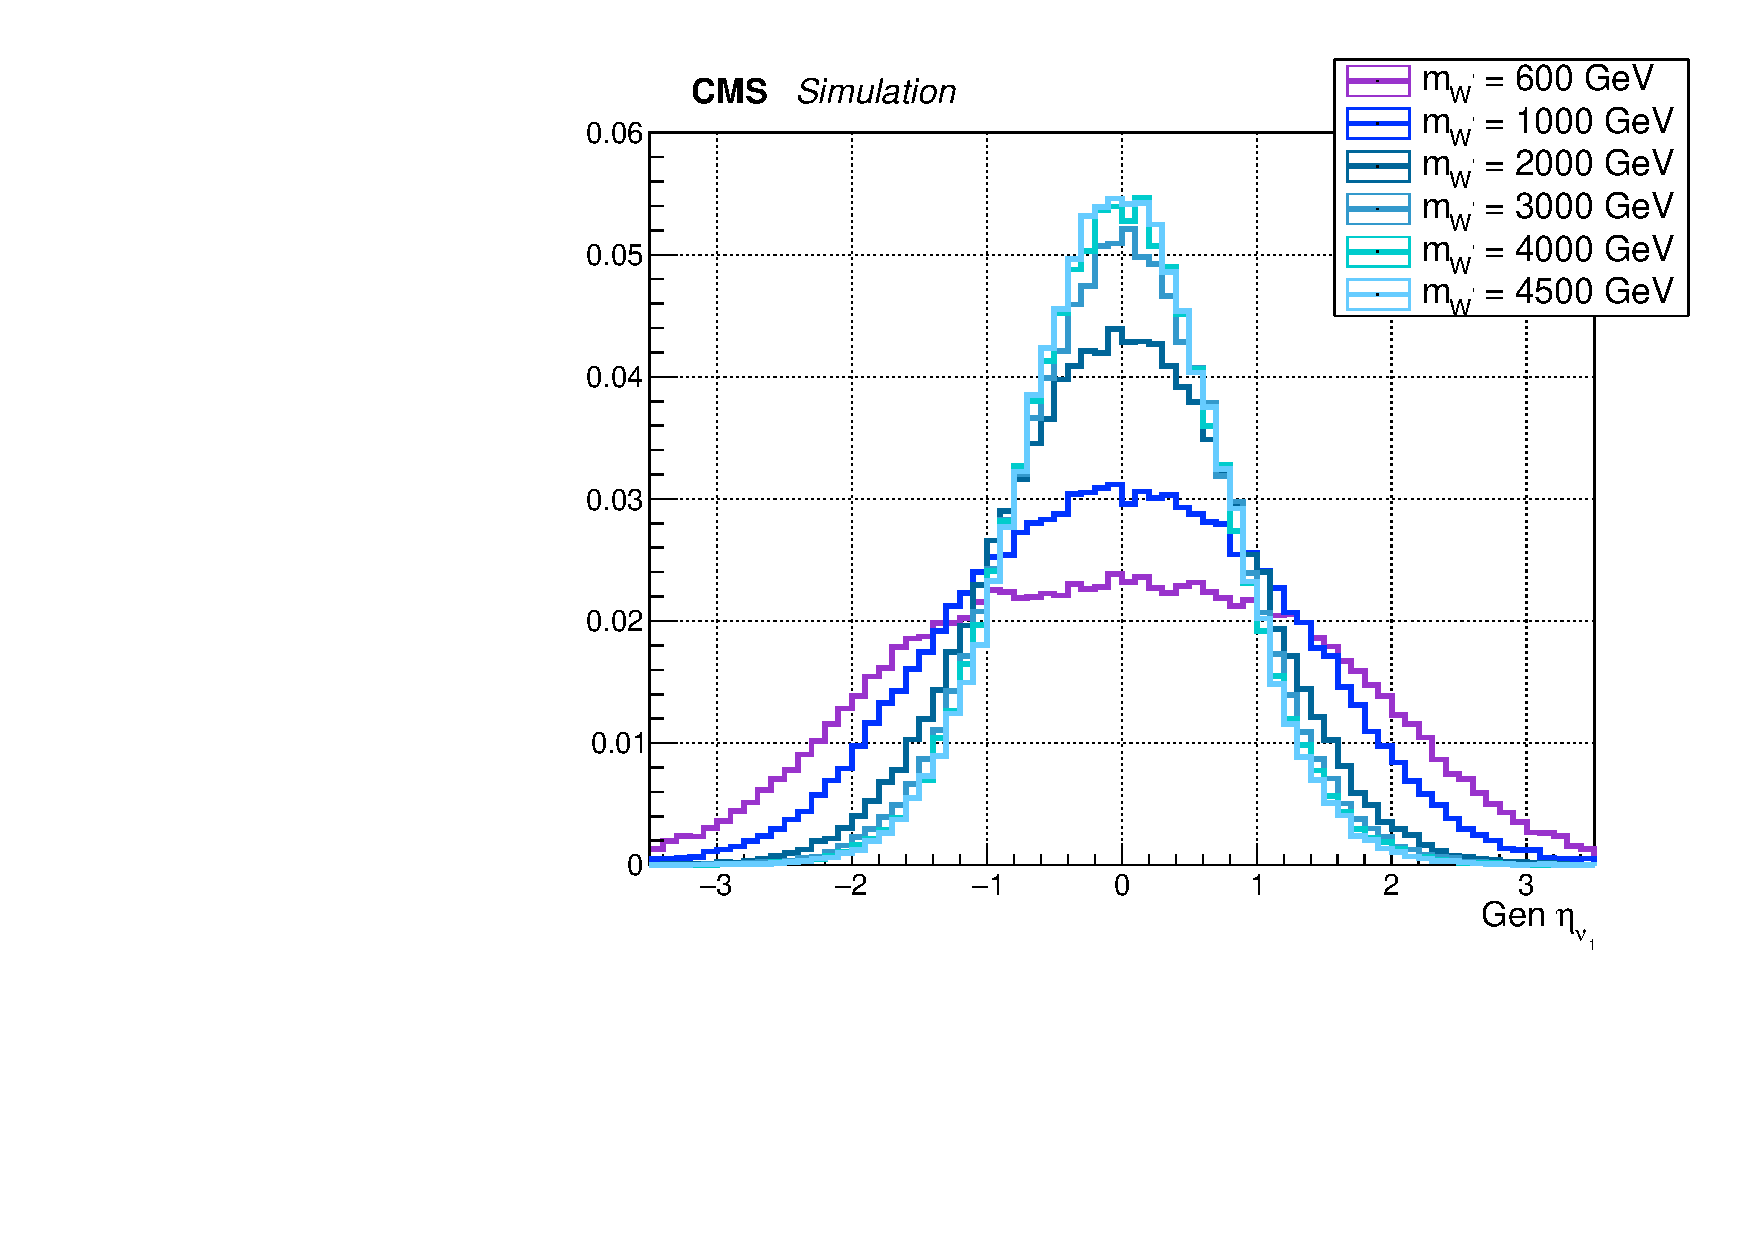
\includegraphics[width=.495\textwidth]{Gen_v9/XWZInv_g_Lep1Eta.pdf}%GenHpt.pdf}
     \\
     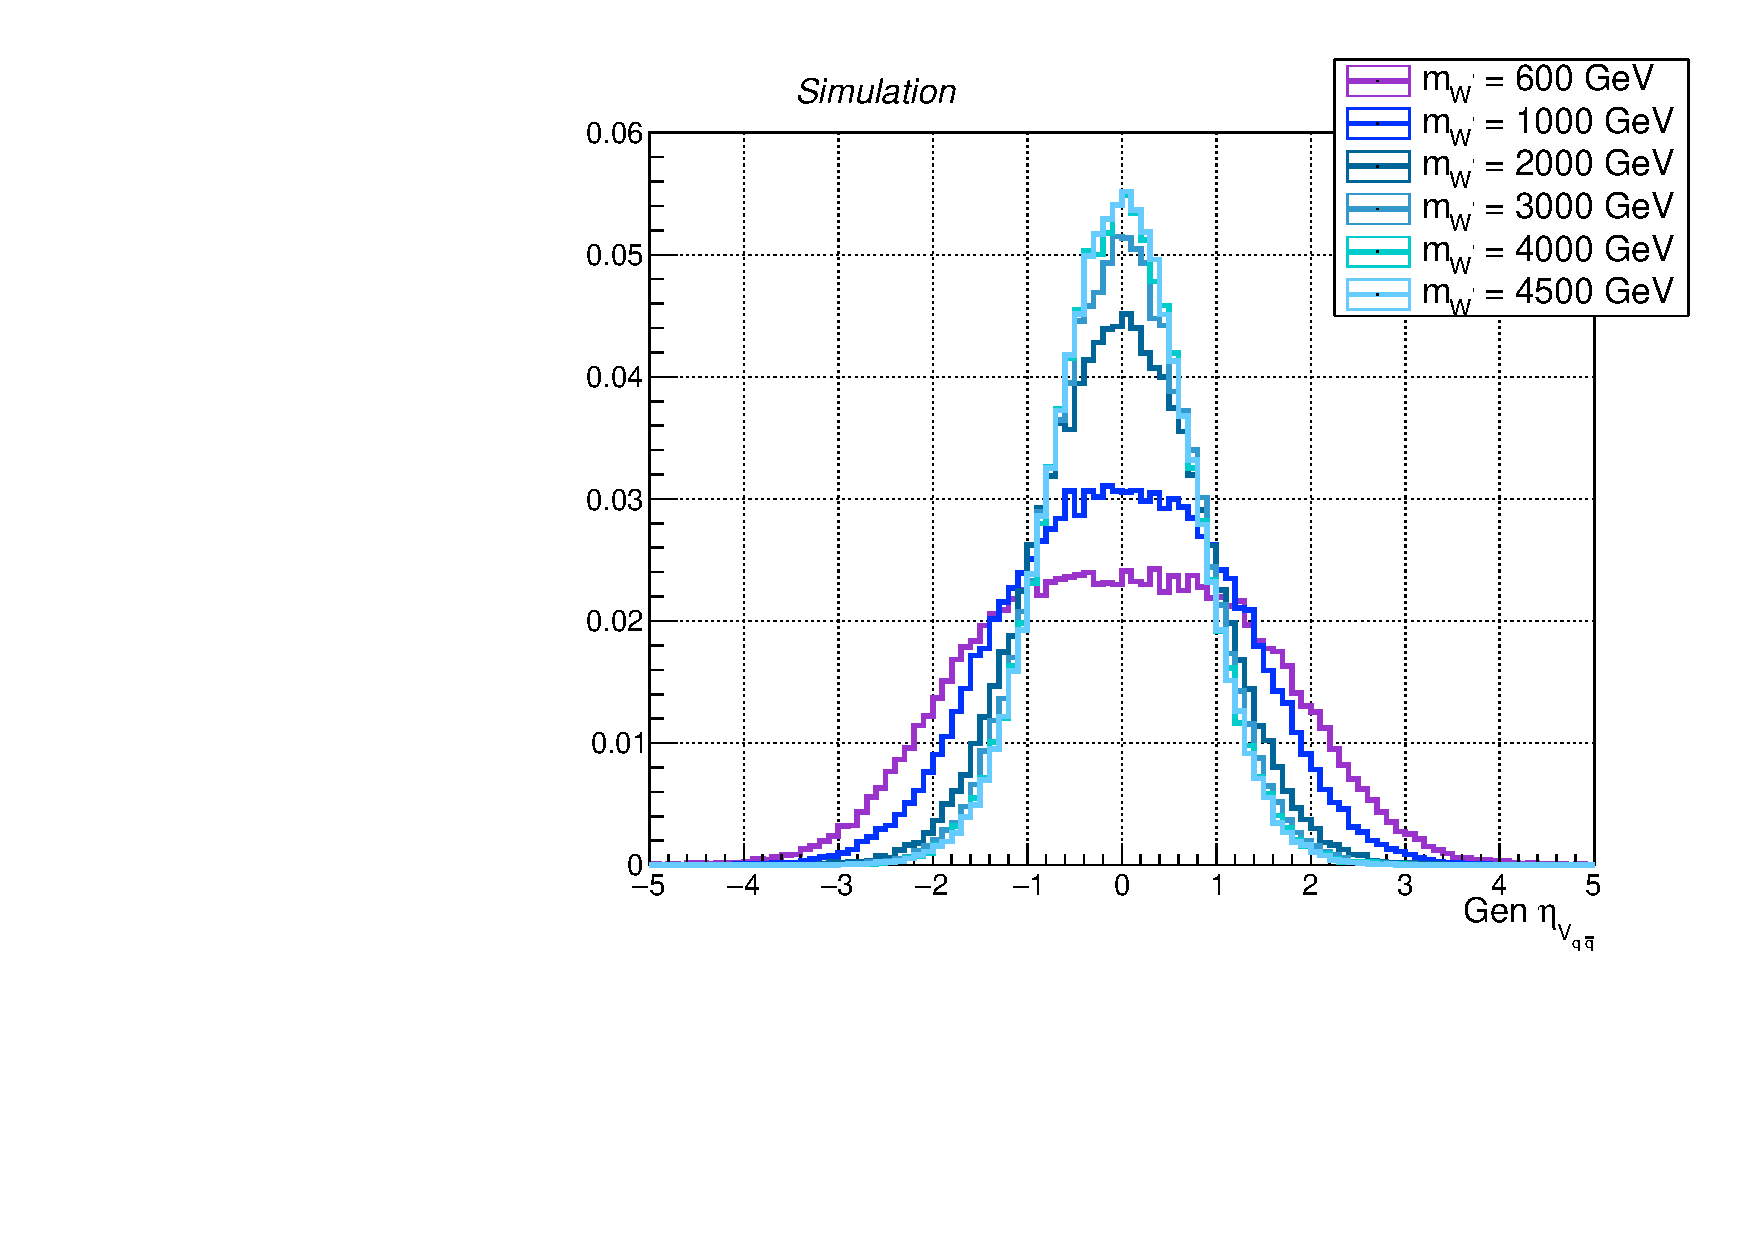
\includegraphics[width=.495\textwidth]{Gen_v9/XWZInv_g_VHadEta.pdf}%GenZdR.pdf}
     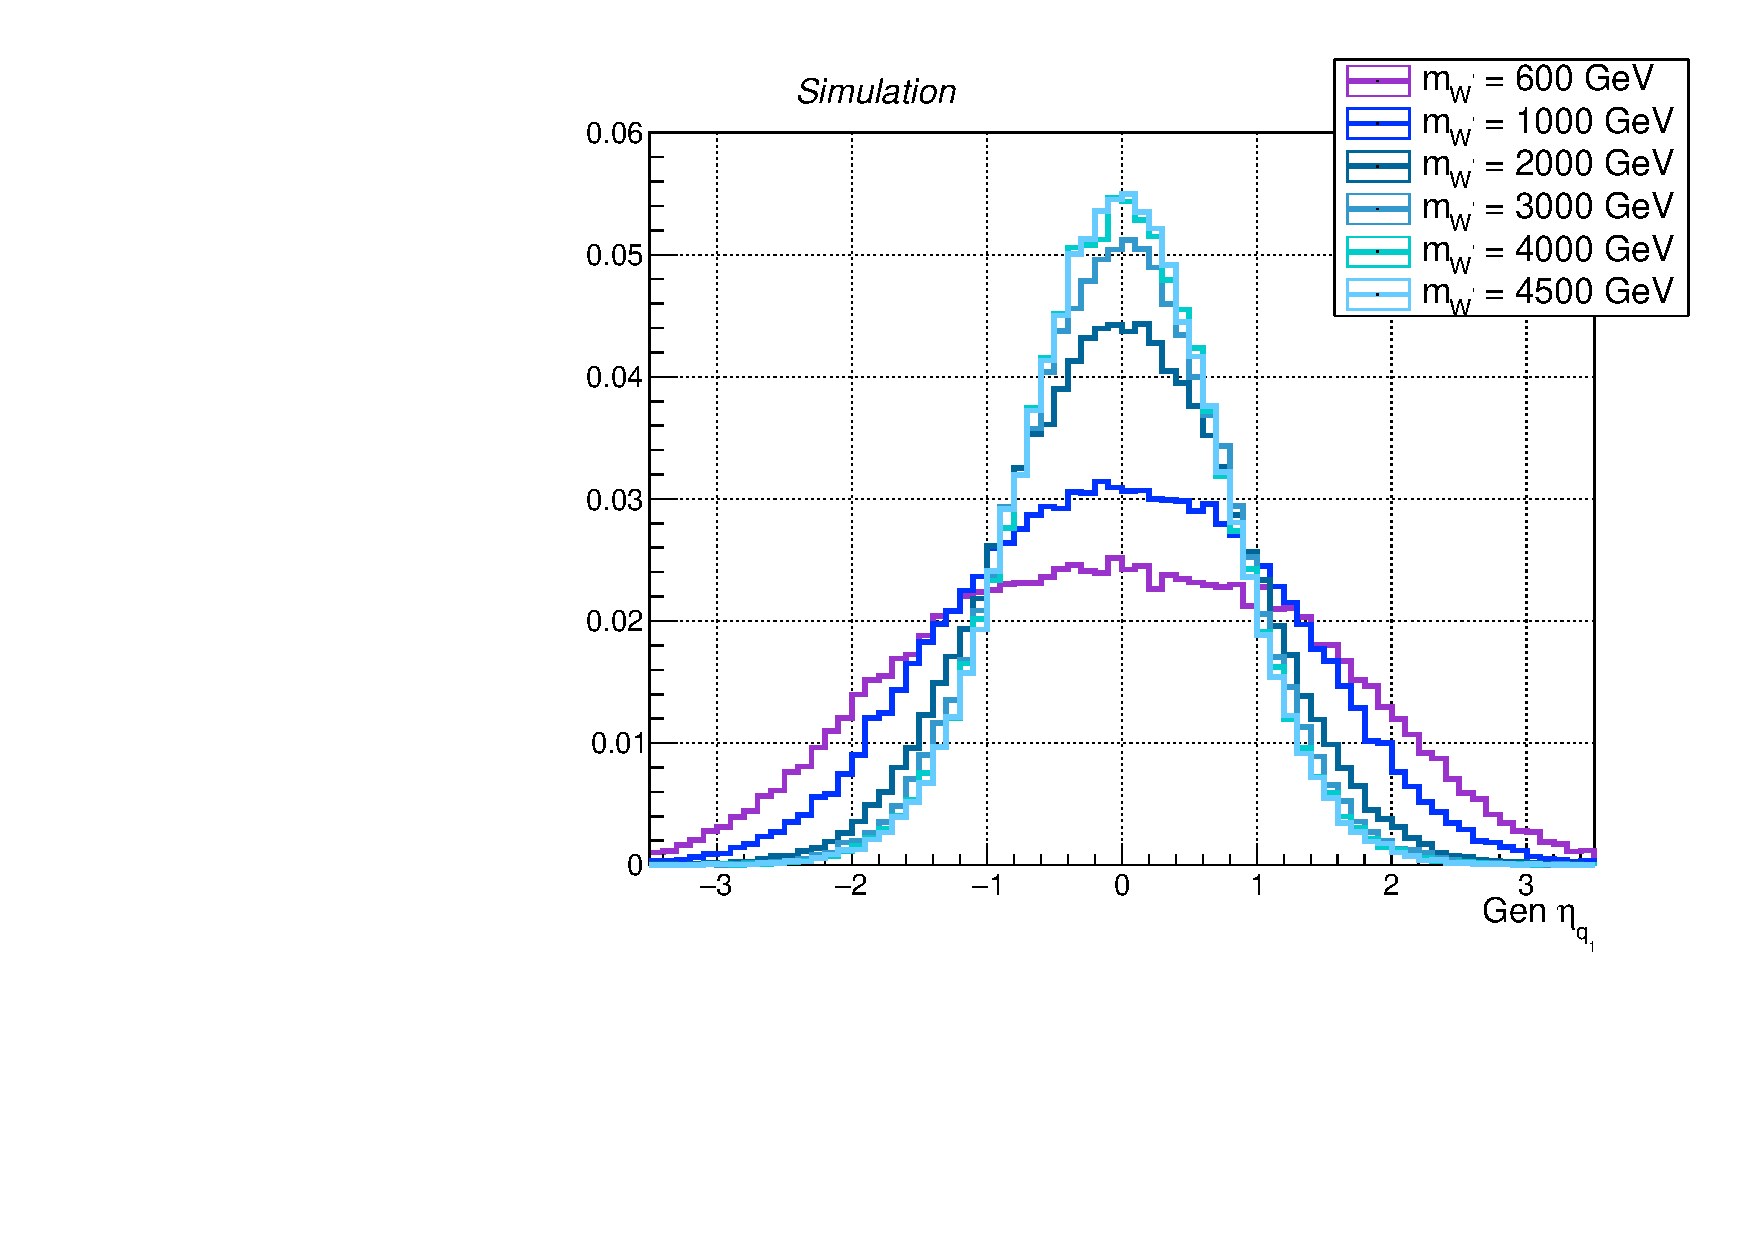
\includegraphics[width=.495\textwidth]{Gen_v9/XWZInv_g_Had1Eta.pdf}%GenHdR.pdf}
   \end{center}
   \caption{Main signal kinematic quantities at generation level after parton showering, for spin-1 \Wp signal, considering different mass hypoteses ($m_{\Wp} = 0.6, 1, 2, 3, 4, 4.5$ TeV). Top: \Wp rapidity $\mathcal{Y}$. Center: pseudorapidity $\eta$ of the invisibly decaying \Z, and pseudorapidity of the leading neutrino. Bottom: pseudorapidity $\eta$ of the hadronically decaying \W, and pseudorapidity of the leading quark.}
   \label{fig:genWprimeSignal2}
 \end{figure}

 \begin{figure}[!htb]
   \begin{center}
     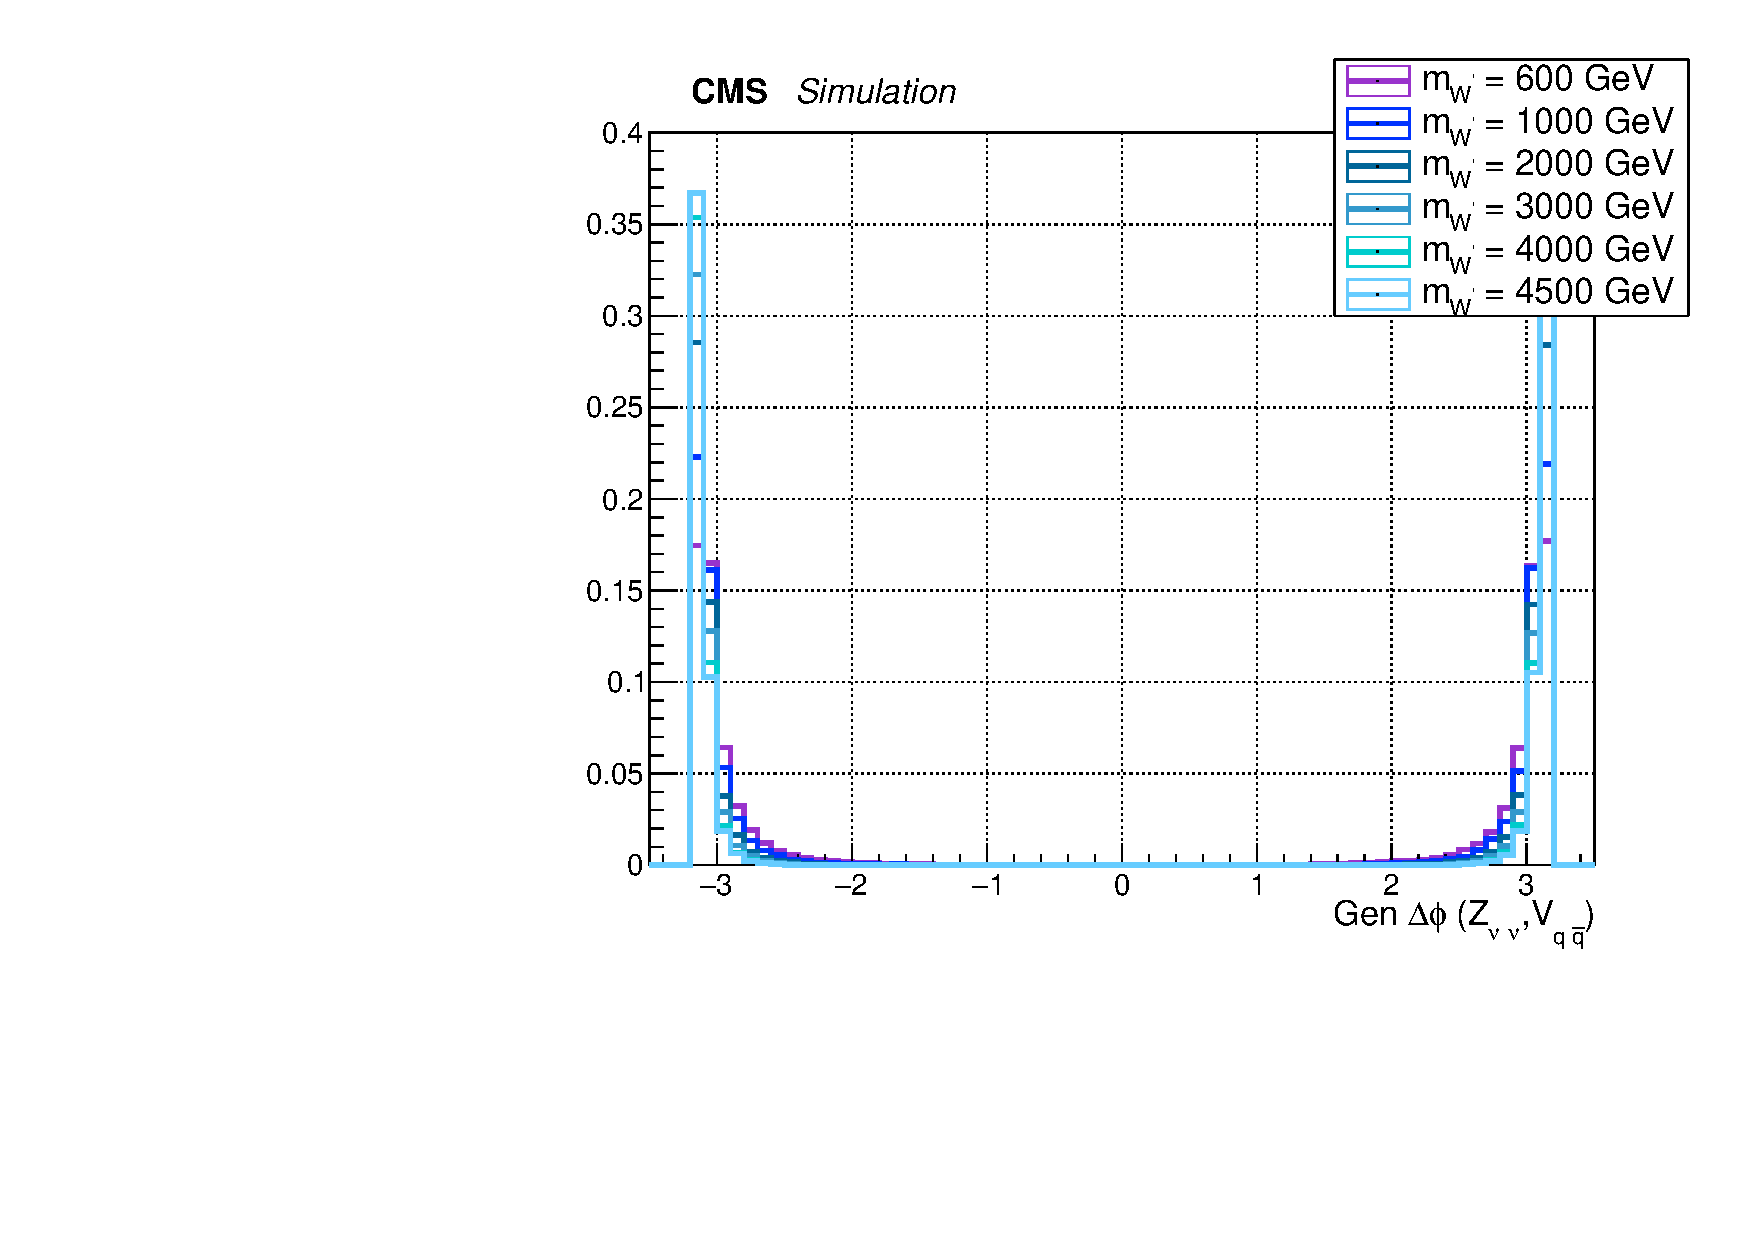
\includegraphics[width=.495\textwidth]{Gen_v9/XWZInv_g_VZDPhi.pdf}%GenPhi1pt.pdf}
     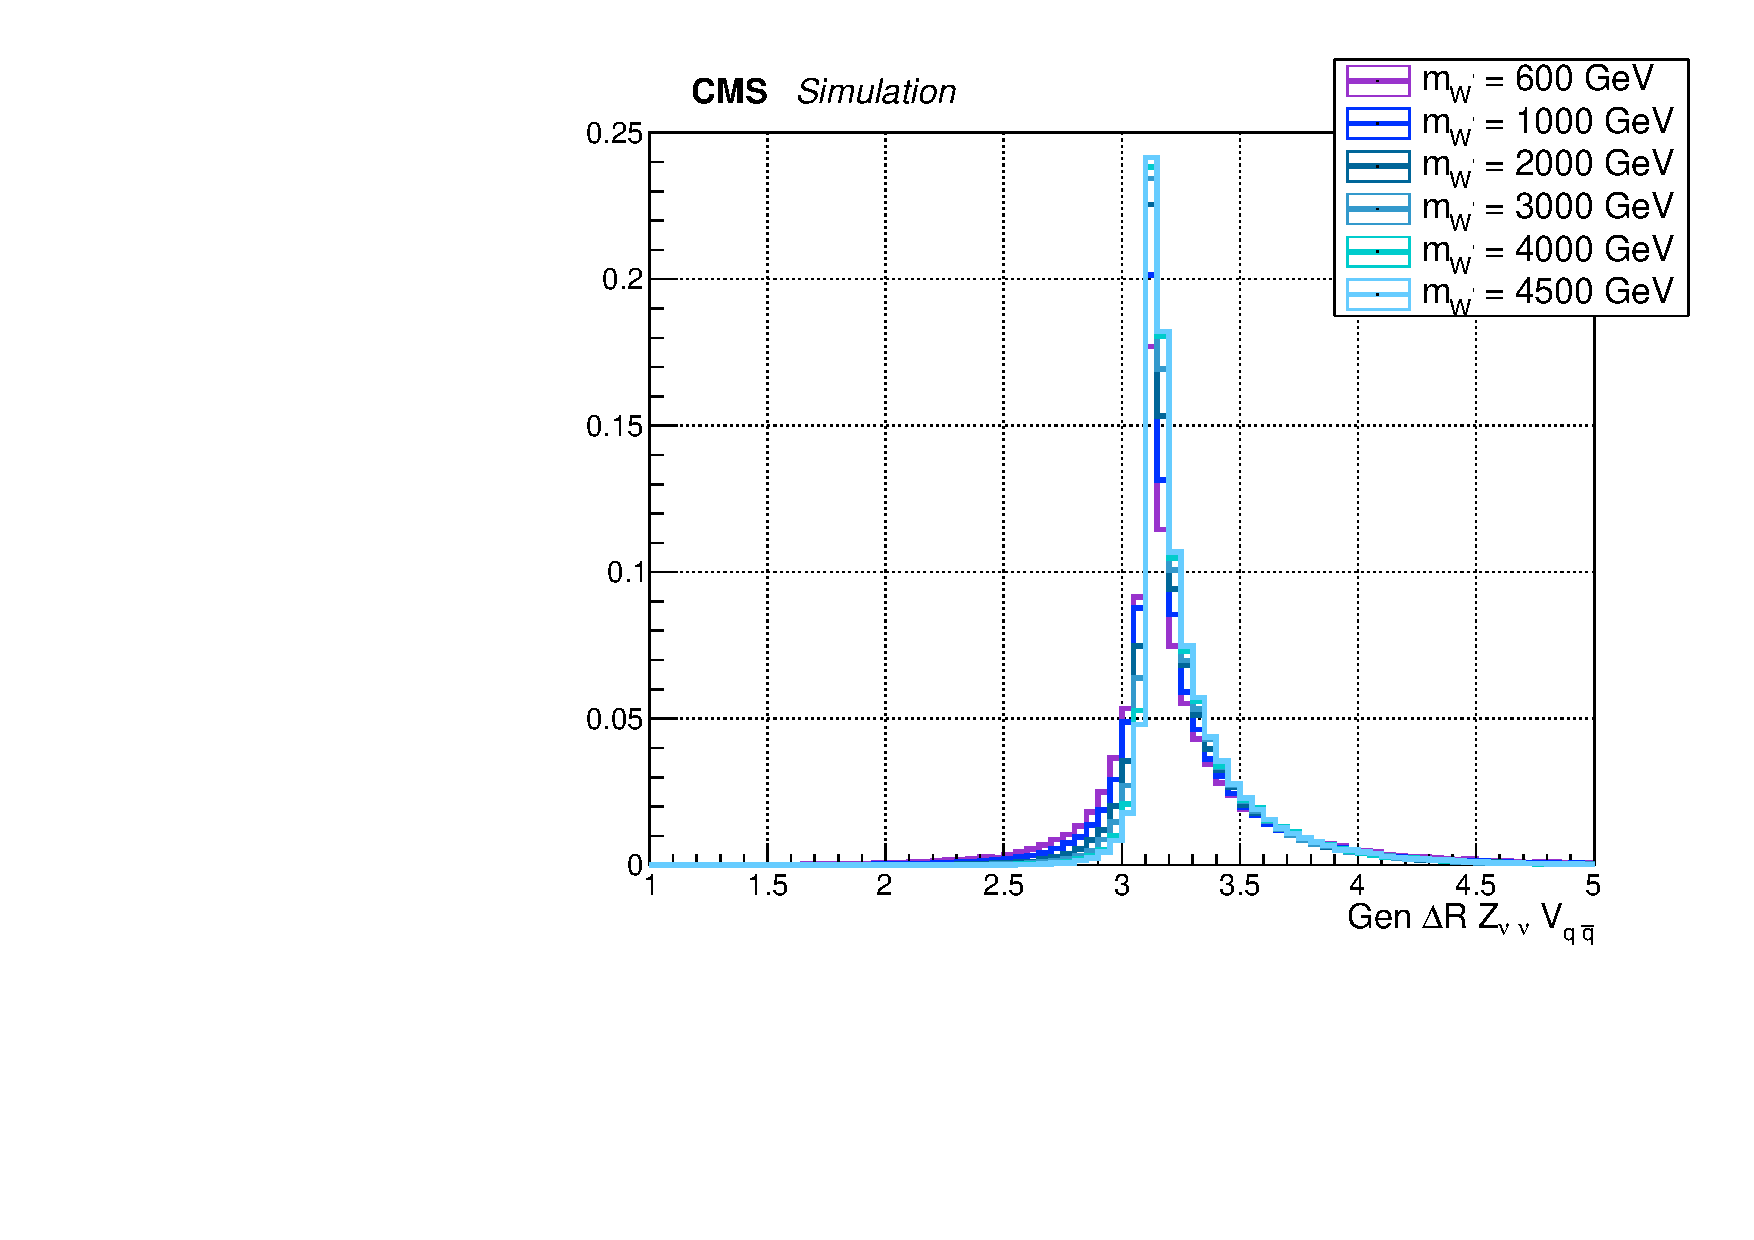
\includegraphics[width=.495\textwidth]{Gen_v9/XWZInv_g_VZDR.pdf}%GenPhi1y.pdf}
     %\\
     %\includegraphics[width=.495\textwidth]{Gen_v7/g_ZLepMass.pdf}%GenZmass.pdf}
     %\includegraphics[width=.495\textwidth]{Gen_v7/g_ZHadMass.pdf}%GenHmass.pdf}
     \\
     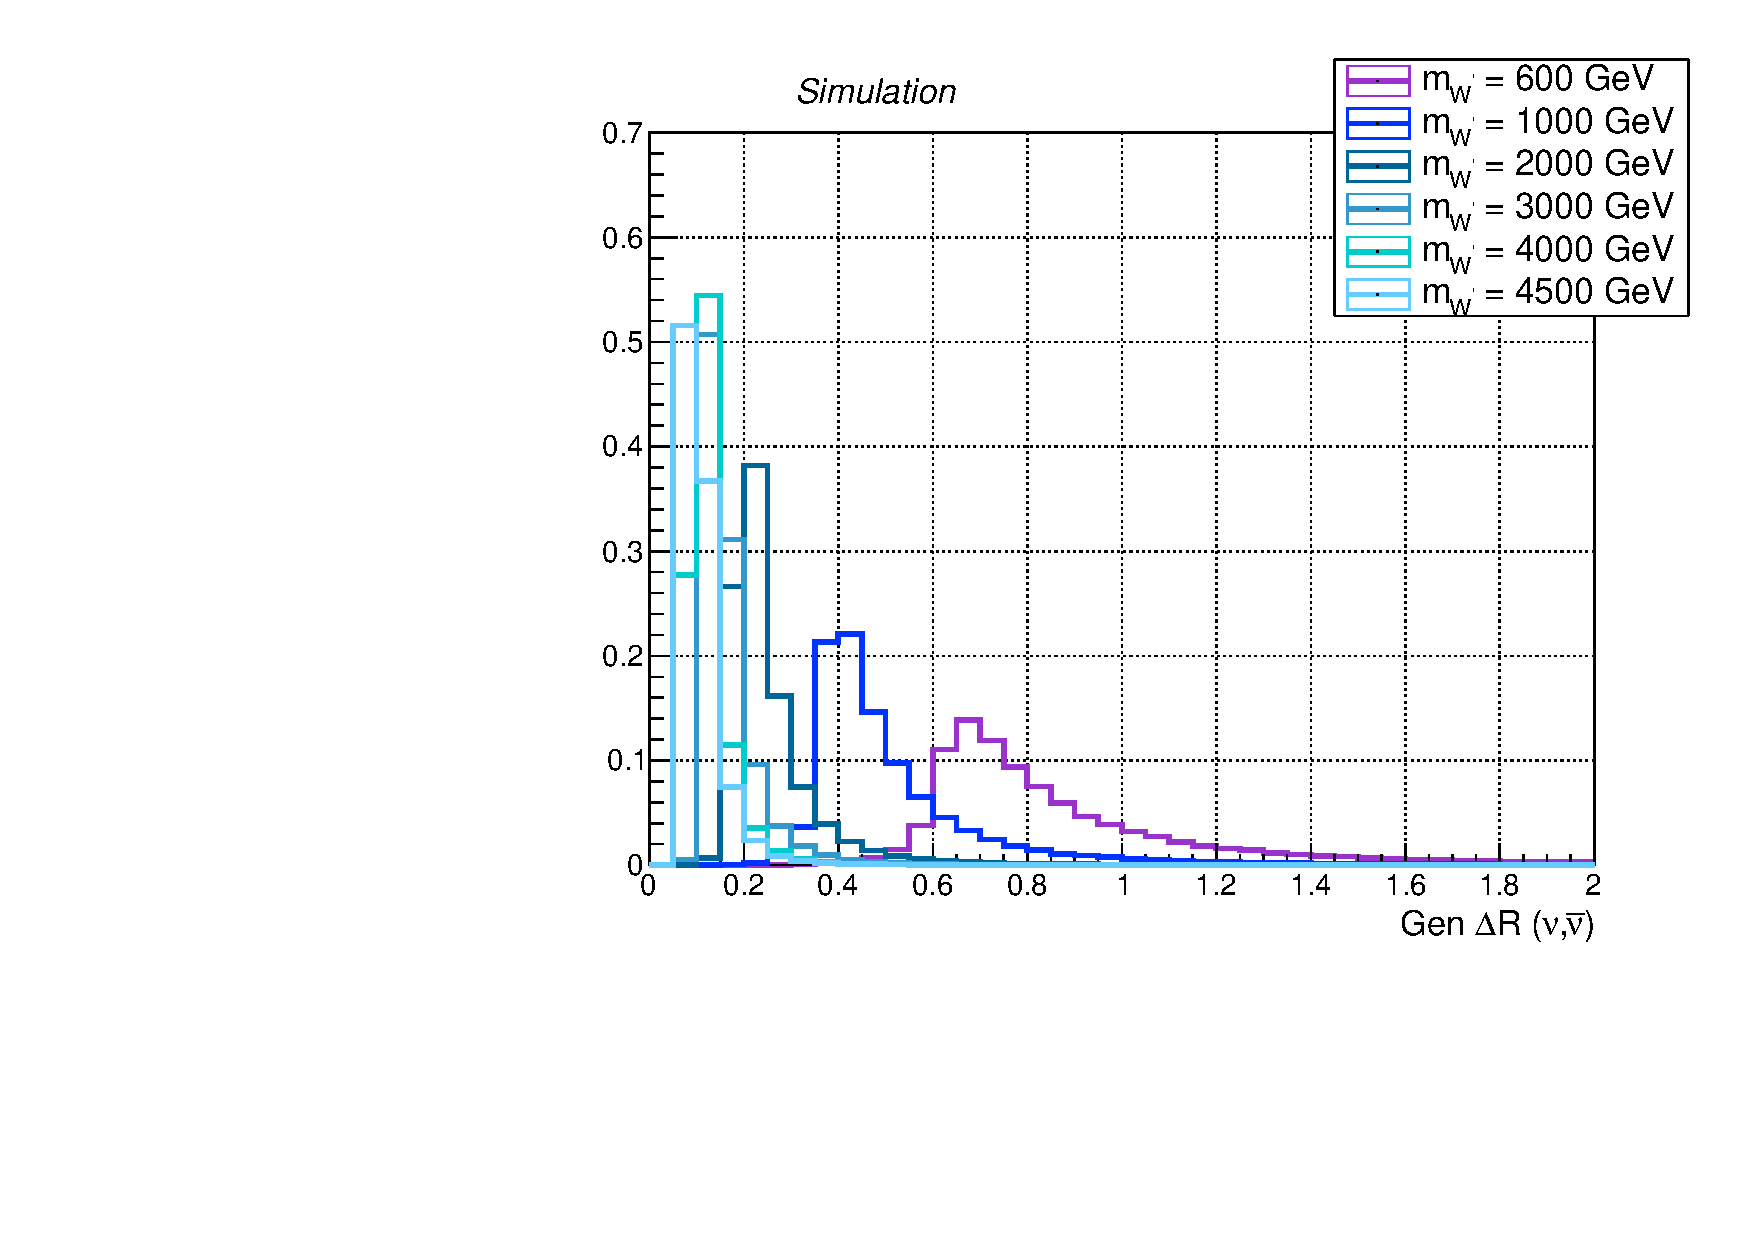
\includegraphics[width=.495\textwidth]{Gen_v9/XWZInv_g_LepDR.pdf}%GenZpt.pdf}
     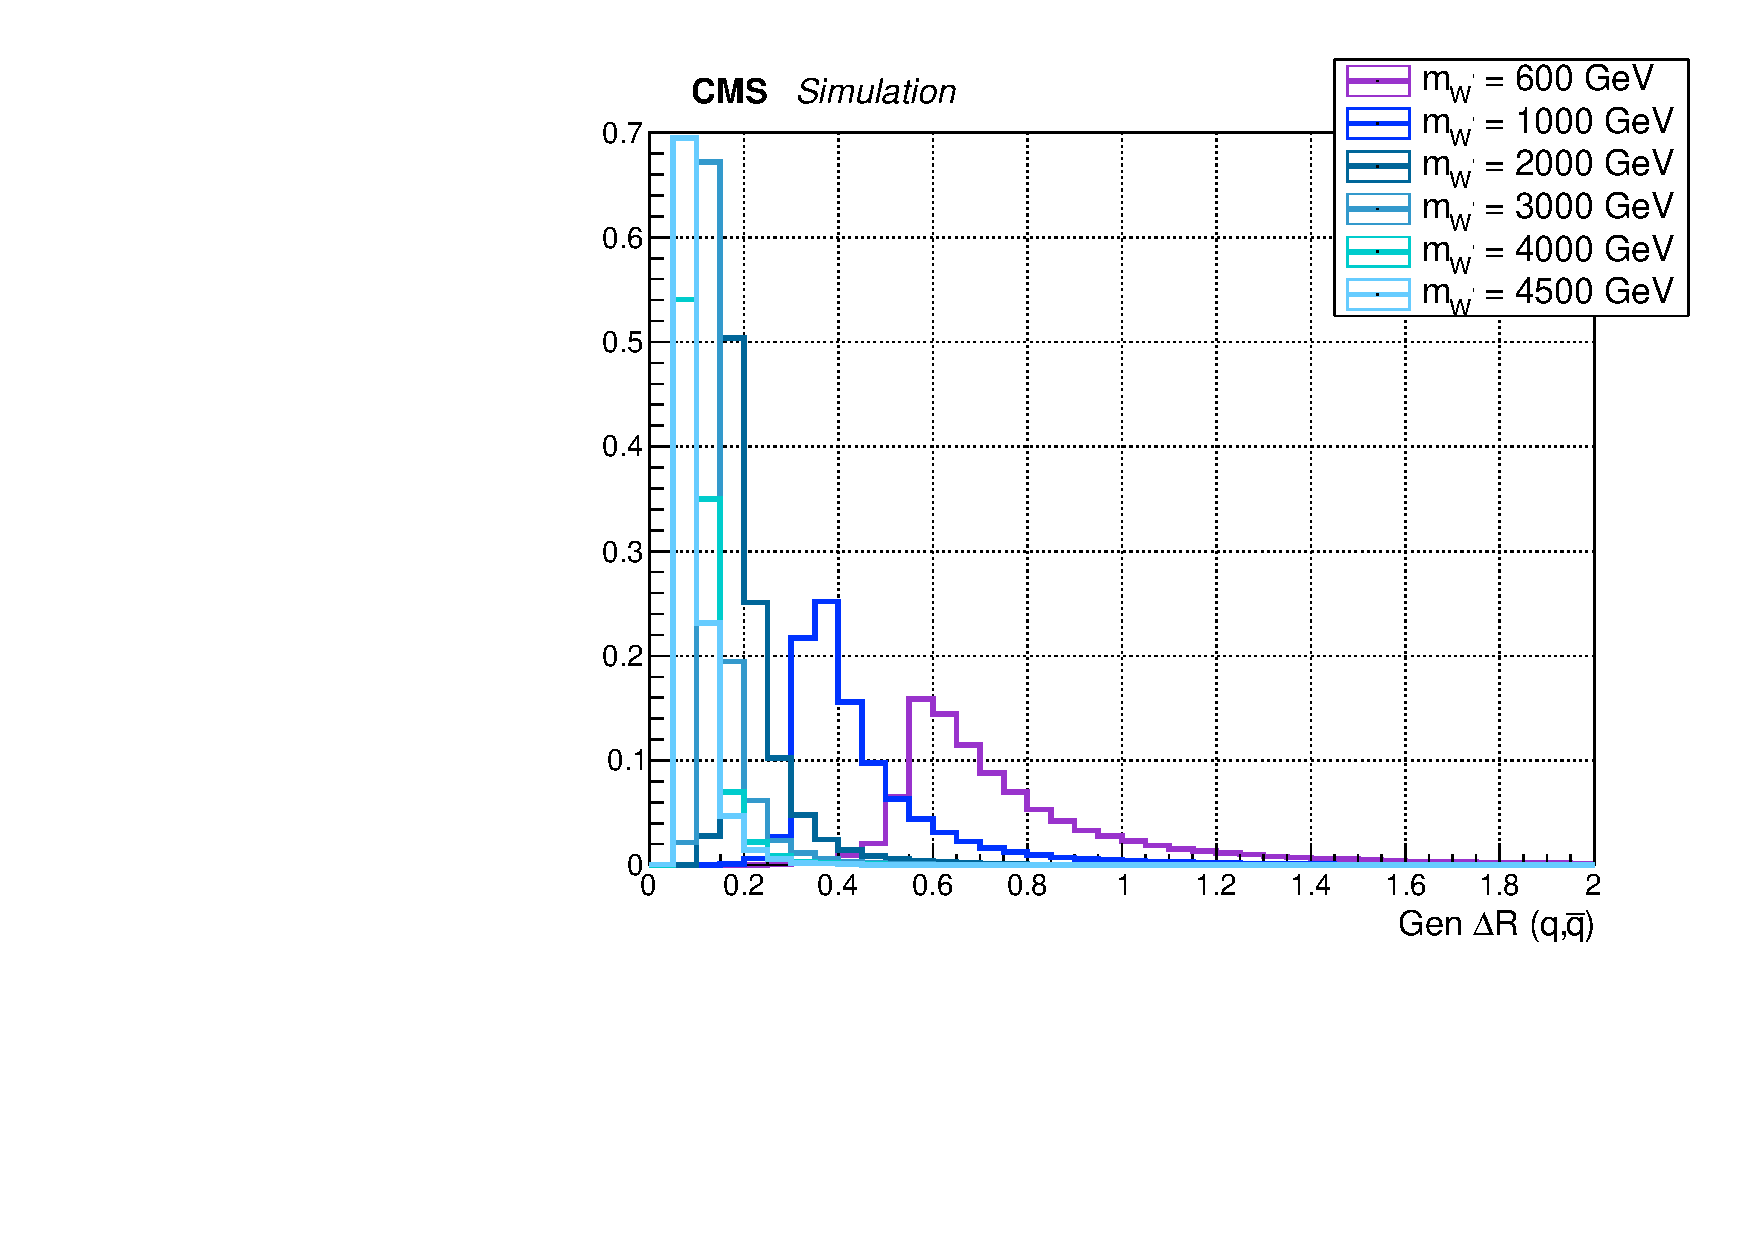
\includegraphics[width=.495\textwidth]{Gen_v9/XWZInv_g_HadDR.pdf}%GenHpt.pdf}
     \\
     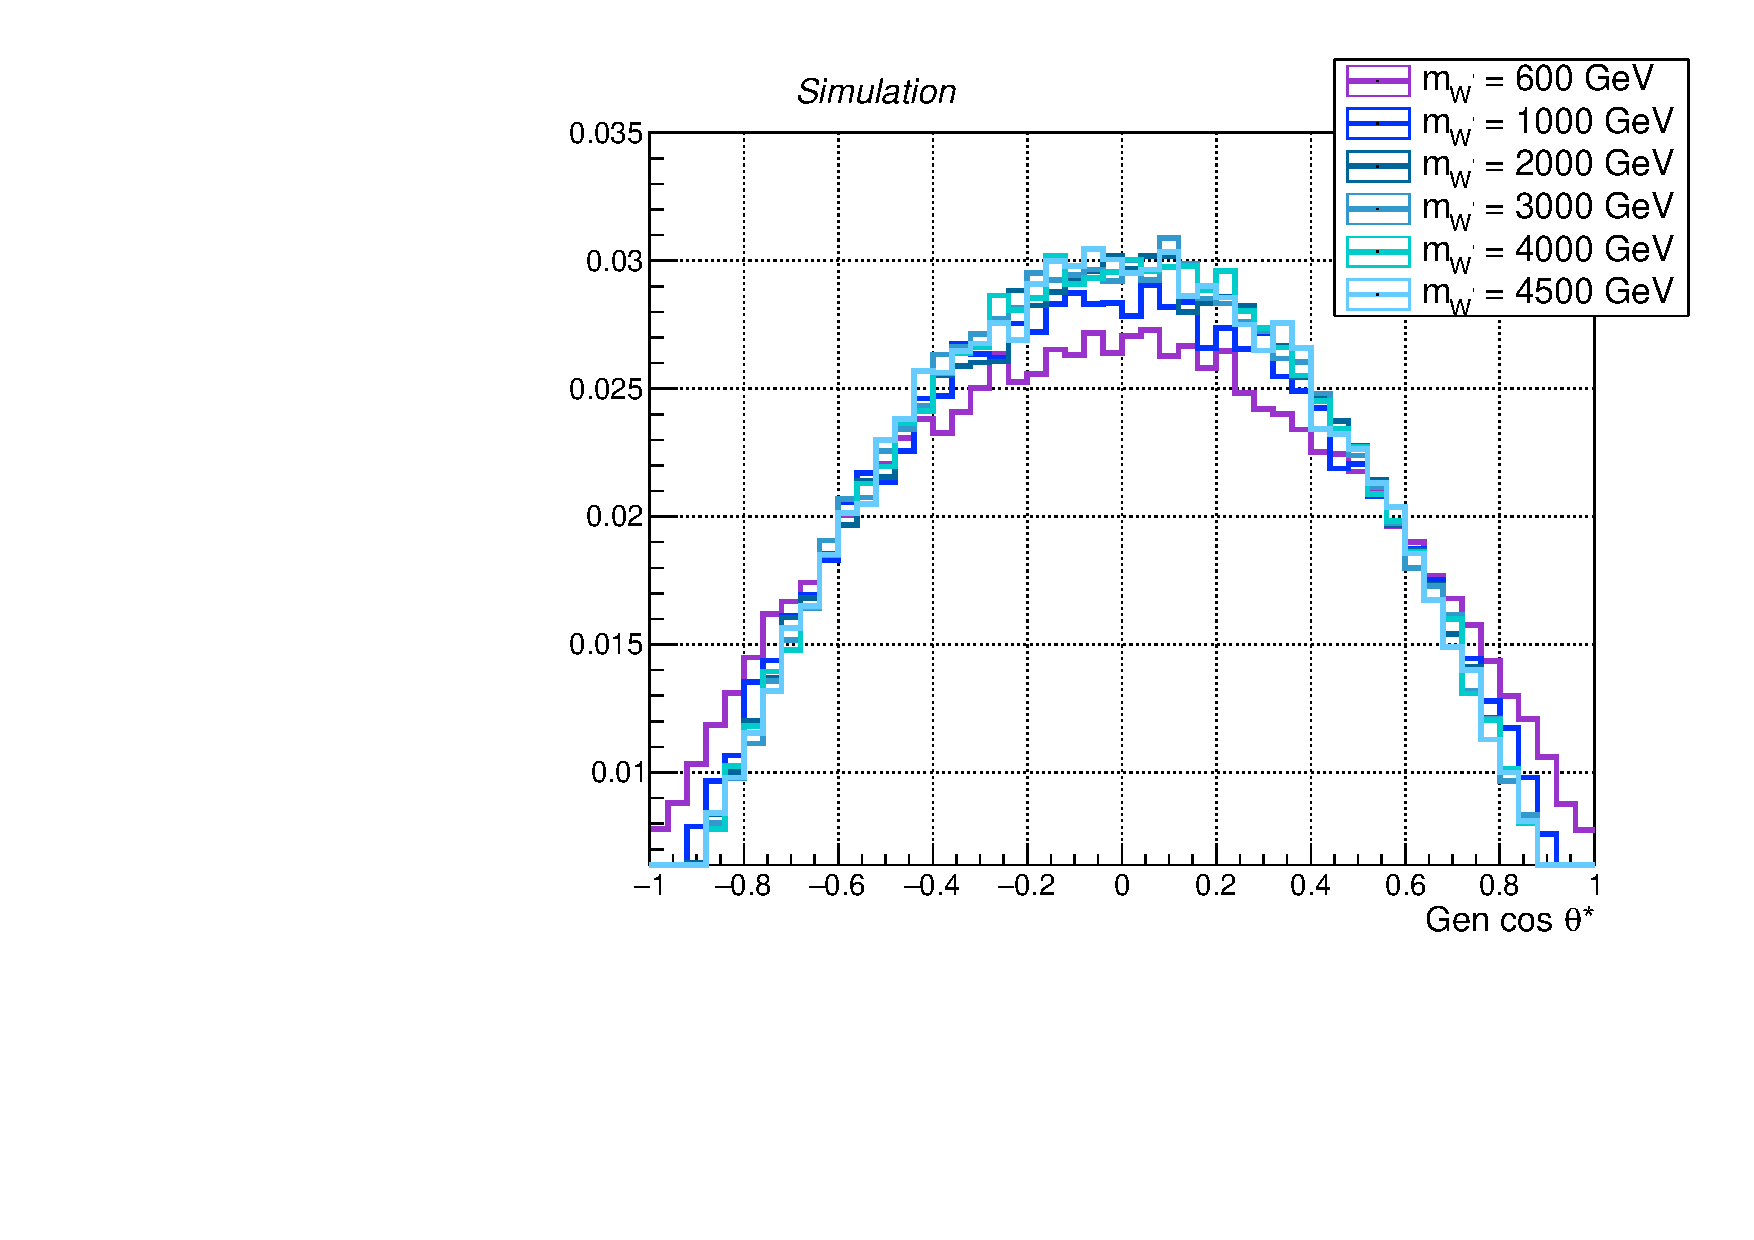
\includegraphics[width=.495\textwidth]{Gen_v9/XWZInv_g_CosThetaStar.pdf}%GenZdR.pdf}
     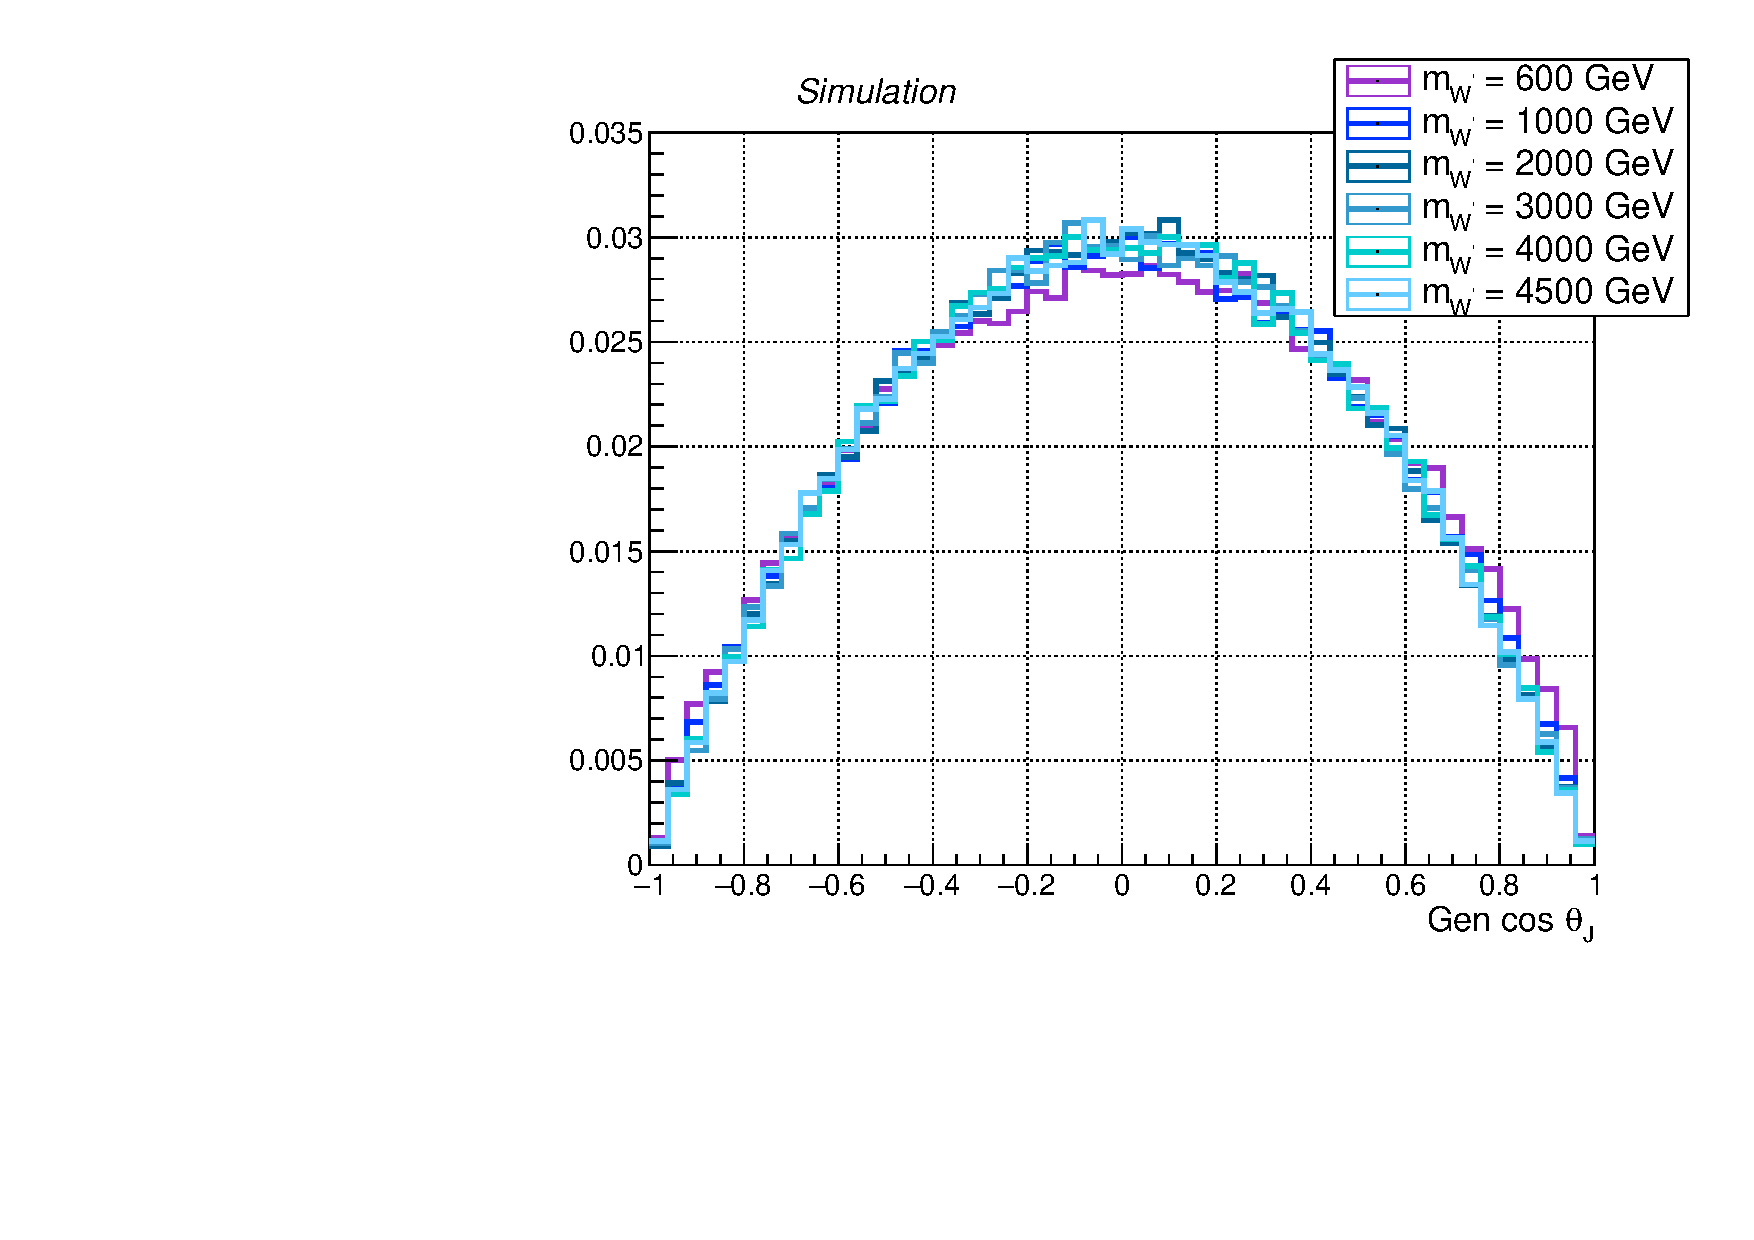
\includegraphics[width=.495\textwidth]{Gen_v9/XWZInv_g_CosThetaJ.pdf}%GenHdR.pdf}
   \end{center}
   \caption{Main signal kinematic quantities at generation level after parton showering, for spin-1 \Wp signal, considering different mass hypoteses ($m_{\Wp} = 0.6, 1, 2, 3, 4, 4.5$ TeV). Top: angular separation in the transverse plane $\Delta \varphi$ (left) and the angle $\Delta R$ (right) between leptonic \Z and hadronic \W. Center: the angle between the neutrinos and the quarks. Bottom: distribution of $\cos{\theta}^{*}$ and $\cos{\theta}_{J}$ (described in text).}
   \label{fig:genWprimeSignal3}
 \end{figure}

\clearpage

\noindent Angular distributions are related to the spin, the polarization and the kinematics of the produced resonance; in particular:
\begin{itemize}
\item $\Delta R$ among neutrinos and quarks reflect the boosted nature of the electroweak bosons: the more massive the resonance, the larger the boost, and hence the closer the fermions. By looking at fig.~\ref{fig:genGravSignal3}-\ref{fig:genWprimeSignal3}, with a jet clustering parameter of 0.8 (AK8 jet) it is possible to enclose the quarks produced by the decay of the \V boson, for a resonance mass over 1 \TeV;
%\item the resonance rapidity $\mathcal{Y}$ is sensitive to the production mechanism
\item $\cos{\theta}^{*}$, namely the cosine of the angle between the momentum of the \V boson, calculated in the resonance rest frame, and the flight direction of the resonance itself in the laboratory frame. This variable depends on the spin of the diboson resonance (spin-2 and spin-1 distributions are different, fig.~\ref{fig:genGravSignal3}-\ref{fig:genWprimeSignal3}). % This variable affects the p T distributions of bosons. When cos θ ∗ = 0, the p T of bosons in the lab frame, for a given X mass, reaches the maximum value and the new resonance X has a symmetric decay where the two bosons have equal p T ’s in the lab frame.
\item $\cos{\theta}_J$, the cosine of the angle between the momentum of the leading quark, calculated in the \V rest frame, and the flight direction of the \V boson in the laboratory frame. This variable depends on the polarization state of the decay bosons~\cite{Khachatryan:2014vla}; in both HVT and bulk graviton model, electroweak bosons are expected to be longitudinally polarized. \W bosons with transverse polarization tend to decay into quarks produced closer to the direction of the boson itself, hence $\left| \cos{\theta}_J \right|$ is peaked at 1; on the other hand, the distribution of $\cos{\theta}_J$ for longitudinally polarized \W bosons is broadly peaked at zero, as in fig.~\ref{fig:genWprimeSignal3}~\cite{Bolognesi:2012mm}. When $\cos{\theta}_J \rightarrow 0$, quarks are produced very close in angle and hence it is difficult to disentangle the two substructures in the large-cone jet (sec.~\ref{ssec:jetsub}); when $\cos{\theta}_J \rightarrow \pi$ the quarks are emitted asymmetrically (one is softer than the other).% asymmetric production -> tau21 can fail. This variable affects the pruned mass and the jet substructure variables (e.g. τ 21 ). The pruning algorithm and the τ 21 selections preferentially select jets that are split more symmetrically, which corresponds to a cos θ 1 value closer to zero.
\end{itemize}
 


\subsection{Background samples}\label{ssec:backgrounds}

The physics processes yielding final states with two neutrinos in association with a pair of quarks are considered as sources of background; they are listed in tab.~\ref{tab:bkg_datasets1}, along with the expected cross-sections at next-to-leading order (NLO) or next-to-next-to leading (NNLO). A summary of the standard model cross-sections, measured by CMS, and their theoretical predictions is included in fig.~\ref{fig:sm_xsec}-\ref{fig:dibjet_xsec}.

\begin{figure}[!htb]
 \centering
   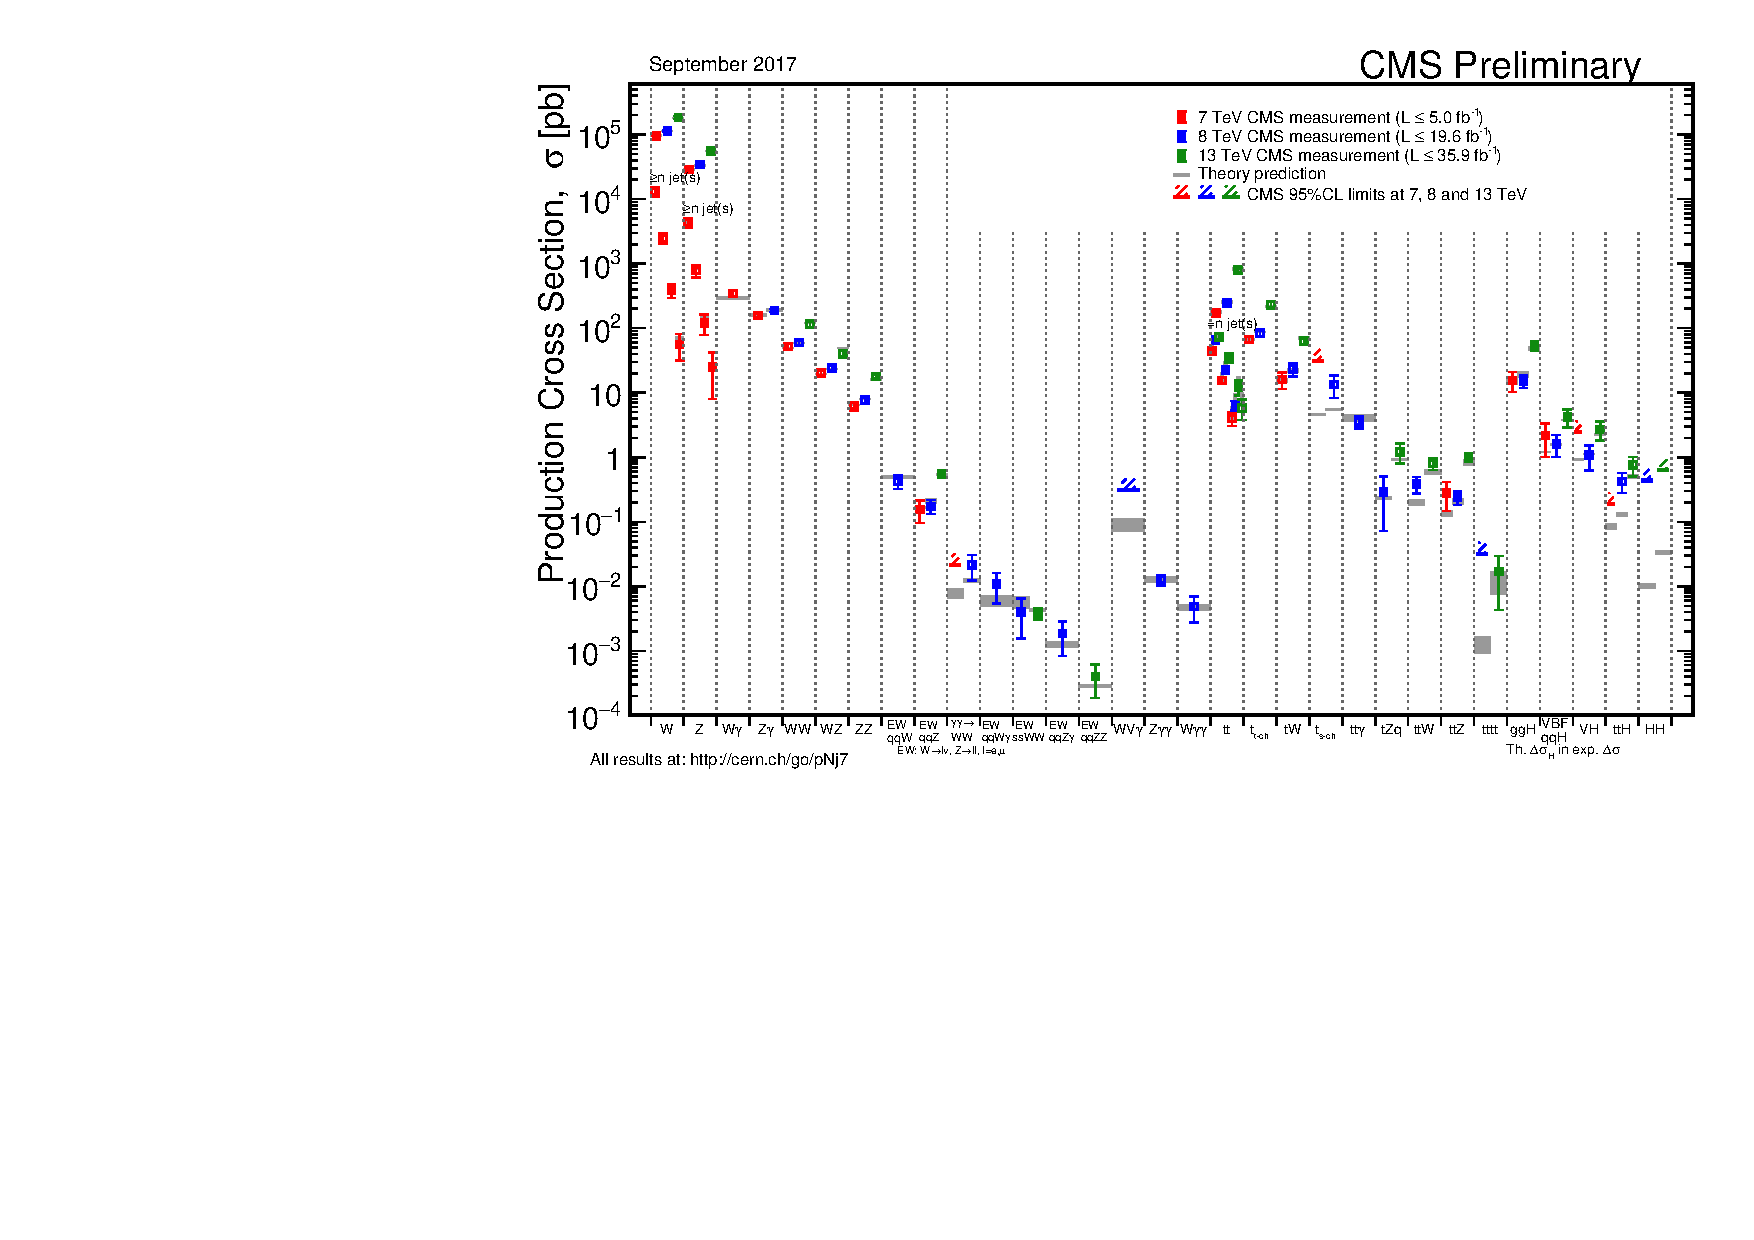
\includegraphics[width=.95\textwidth]{figures/SigmaNew_v0.pdf}
 \caption{Production cross-sections of the main standard model processes, as measured by CMS, and theoretical predictions.}
 \label{fig:sm_xsec}
\end{figure}

\begin{figure}[!htb]
 \centering
   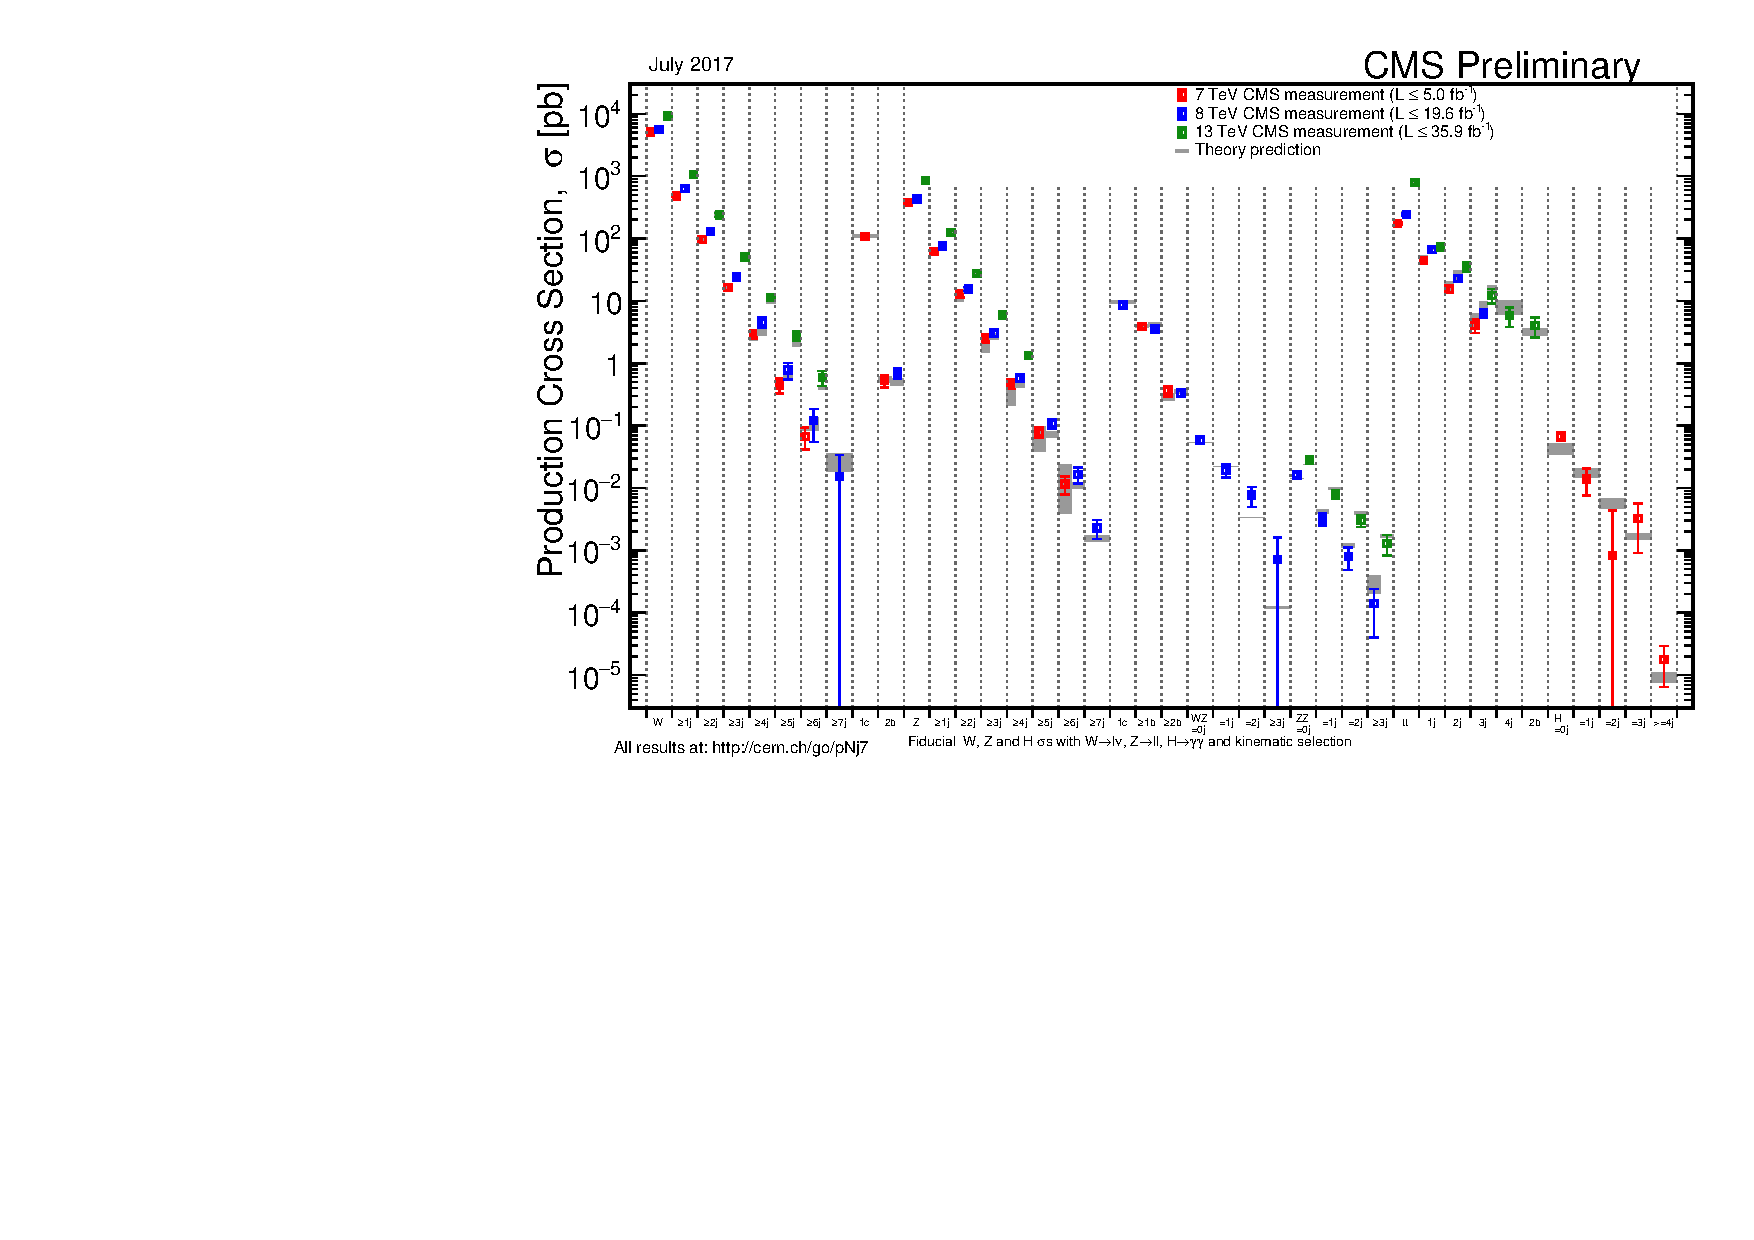
\includegraphics[width=.95\textwidth]{figures/SigmaNew_v3.pdf}
 \caption{Production cross-sections of the standard model processes involving a vector boson in association with jets, as measured by CMS, and theoretical predictions. These phenomena represent the main background sources for the analysis.}
 \label{fig:dibjet_xsec}
\end{figure}

%\begin{figure}[!htb]
% \centering
%   \includegraphics[width=.95\textwidth]{figures/SigmaNew_v8.pdf}
% \caption{...}
% \label{fig:top_xsec}
%\end{figure}

\begin{itemize}
  \item {\bf \Z + jets}: this process represents the main irreducible background for the signal. The production of a \Z boson in association with one or more partons in the final state has topology that is similar to the signal. This \Z + jets background is produced in samples binned in \pt of the \Z boson, starting from 100 \GeV, with the {\sc aMC@NLO} generator, with FXFX merging~\cite{bib:FXFX}. The contribution from events with $\pt<100$~GeV is negligible after the requirement on the \met to be greater than 200~\GeV (sec.~\ref{sec:selections}).

  \item {\bf \W + jets}: the leptonic decay of a \W boson can be an irreducible background if the charged lepton escapes undetected (\textit{i.e.} outside the detector acceptance) or fails the lepton identification requirements. The production of a \W boson has a cross section larger by an order of magnitude with respect to the \Z, and this makes the \W + jets a relevant background also when a lepton veto is applied. This \W + jets background is produced in samples binned in \pt of the \W boson, starting from 100 \GeV, with the {\sc aMC@NLO} generator.% \W + jets background binned in \HT (the sum of the \pt of the hadrons at generator level) starting from 100 \GeV with the \MADGRAPH LO generator are kept as backup samples.
  \item $\mathbf{Top}$: pair and single production of top quarks represent a source of background, due to the production of a \W boson in 100\% of top decays, $t \rightarrow b \W$. \ttbar pair production results in two b-jets and two \W bosons in the final state, that can decay to leptons that escape the detector or fail to be identified as leptons. This analysis makes use of \ttbar inclusive decays samples based on \POWHEG v2~\cite{bib:POWHEGst} NLO generator. Single-top and single-antitop samples are produced in the 5-flavours scheme using \POWHEG v2~\cite{bib:POWHEGtt} NLO generator. Different production mechanisms are considered: $t \W$ channel, when a top quark is produced in association with a \W boson, due to a gluon-bottom quark scattering; s-channel, due to quark-antiquark scattering, producing a top and an anti-bottom quark in the final state; t-channel, via a virtual \W in a quark-b-quark scattering, resulting in a top quark and a quark jet in the final state.
  \item {\bf Diboson}: the SM production of a pair of vector bosons is topologically close to the searched signal, by the way the cross-section of the process is low. $WW$ production is the most probable process, that imitates the signal when one of the \W decays leptonically and the charged lepton fall outside the detector acceptance or it is mis-identified; $WZ$ and $ZZ$ processes have smaller cross-sections but are topologically identical to the signal, except for the fact that the invariant mass of the diboson system has a smoothly falling spectrum, in contrast to the resonant signal distribution. Inclusive diboson production processes ($WW$, $WZ$, $ZZ$) are simulated at LO by \PYTHIA generator.
  \item {\bf Multi-jet}: despite the very large cross-section, this source of background is suppressed by a dedicated selection and hence negligible for the analysis (sec.~\ref{sec:selections}).
\end{itemize}




%\begin{sidewaystable}[!htb]\centering
\begin{table}[!htb]\centering
\caption{Simulated Monte Carlo samples. The cross-section $\times$ branching fraction for each process is shown in \pb.\label{tab:bkg_datasets1}}
\begin{tabular}{l|cccc}
 Signal process &  Kinematical cuts & Generator & $\sigma\times\mathcal{B}$ [pb] & N of events \\
 \hline 
 \hline 
$Z \rightarrow \nu \nu$ + jets & $100 < p_{T,Z} < 250$ \GeV & amcatnloFXFX -- Pythia8 &170.4 & 10710313\\
$Z \rightarrow \nu \nu$ + jets & $250 < p_{T,Z} < 400$ \GeV & amcatnloFXFX -- Pythia8 & 6.636 & 2112619\\
$Z \rightarrow \nu \nu$ + jets & $400 < p_{T,Z} < 650$ \GeV & amcatnloFXFX -- Pythia8 & 0.9372 & 1101297\\
$Z \rightarrow \nu \nu$ + jets & $p_{T,Z} > 650$ \GeV & amcatnloFXFX -- Pythia8 & 0.1042 & 2047215\\
\hline
$W \rightarrow \ell \nu$ + jets & $100 < p_{T,W} < 250$ \GeV & amcatnloFXFX -- Pythia8 & 676.3 & 20178260\\
$W \rightarrow \ell \nu$ + jets & $250 < p_{T,W} < 400$ \GeV & amcatnloFXFX -- Pythia8 & 23.94 & 2001382\\
$W \rightarrow \ell \nu$ + jets & $400 < p_{T,W} < 650$ \GeV & amcatnloFXFX -- Pythia8 & 3.031 & 1939947\\
$W \rightarrow \ell \nu$ + jets & $p_{T,W} < 650$ \GeV & amcatnloFXFX -- Pythia8 & 0.4524 & 1974609\\
%%
%%
%WJetsToLNu\_HT-100To200\_TuneCUETP8M1\_13TeV-madgraphMLM-pythia8\_ext1-v1 & 1292.0 & 35244500 \\
%WJetsToLNu\_HT-200To400\_TuneCUETP8M1\_13TeV-madgraphMLM-pythia8\_ext1-v1 & 385.9 & 19851624 \\
%WJetsToLNu\_HT-400To600\_TuneCUETP8M1\_13TeV-madgraphMLM-pythia8-v1 & 47. & 7432746 \\
%WJetsToLNu\_HT-600To800\_TuneCUETP8M1\_13TeV-madgraphMLM-pythia8-v1 & 12.8 & 3722395\\
%WJetsToLNu\_HT-800To1200\_TuneCUETP8M1\_13TeV-madgraphMLM-pythia8-v2 & 5.261 & 1540477 \\
%WJetsToLNu\_HT-1200To2500\_TuneCUETP8M1\_13TeV-madgraphMLM-pythia8\_ext1-v1 & 1.334 & 7063909\\
%WJetsToLNu\_HT-2500ToInf\_TuneCUETP8M1\_13TeV-madgraphMLM-pythia8-v1 & 0.03089 & 2254248 \\
\hline
\ttbar inclusive & - & Powheg -- Pythia8 & 831.76 & 77229341 \\
\hdashline
$t$ ($tW$ channel) & - & Powheg -- Pythia8 & 35.85 & 6952830\\
5f inclusive \\
\hdashline
$\bar{t}$ ($\bar{t}W$ channel) & - & Powheg -- Pythia8 & 35.85 & 6933094\\
5f inclusive \\
\hdashline
$t$ (s-channel) & - & amcatnloFXFX -- Pythia8 & 3.344 & 622990\\
4f lepton decays \\
\hdashline
$t$ (t-channel) & - & Powheg -- Madspin -- & 136.02 & 67240808 \\
4f inclusive & & -- Pythia8  & & \\
\hdashline
$\bar{t}$ (t-channel) & - & Powheg -- Madspin -- & 80.95 & 38811017\\
4f inclusive & & -- Pythia8  & & \\
\hline
$WW$ inclusive & - & Pythia8 & 118.7 & 7981136\\
$WZ$ inclusive & - & Pythia8 & 47.2 & 3995828\\
$ZZ$ inclusive & - & Pythia8 & 16.6 & 1988098\\

\end{tabular}
%\end{sidewaystable}
\end{table}

%\clearpage

\subsection{Vector boson momentum corrections}

%\subsubsection{NLO electroweak corrections}

Corrections to the \pt spectrum of the \V boson, due to NLO electroweak contributions, are enhanced at \TeV scale~\cite{Kallweit:2015fta}, and they become significant for the purpose of this search. These corrections are effectively applied on a per-event basis, depending on the \pt of the vector boson at generation level. Figure~\ref{fig:ewk} shows the amount of the corrections for the \W and \Z bosons.

\begin{figure}[!htb]
 \centering
   \includegraphics[width=.495\textwidth]{figures/EWK.pdf}
 \caption{Electroweak corrections for the \Z (green line) and \W boson (purple line) as a function of the transverse momentum of the boson~\cite{Kallweit:2015fta}.}
 \label{fig:ewk}
\end{figure}


%\clearpage

\subsection{Data samples}
\label{sec:data}

The data used in this analysis have been collected during proton-proton collisions produced at LHC in 2016, at a center-of-mass energy of 13 TeV, with colliding bunches spaced by 25 ns, and with the CMS solenoid enabled. Three group of datasets have been considered:
\begin{itemize}
\item the {\tt MET} dataset, where the analysis is performed, is collected by triggers requiring a large amount of \met at HLT level in the event;
\item the {\tt SingleMuon} dataset, used to perform an unbiased trigger efficiency estimate, is collected by triggers requiring at least one well defined muon at HLT level;
\item the {\tt SingleElectron} dataset, used as cross-check for the trigger efficiency estimation, is collected by triggers requiring at least one well defined electron at HLT level.
\end{itemize}

\noindent Data selected for the analysis include all the runs certified as ``good'' for all subsystems. The corresponding integrated luminosity amounts to $35.9 \pm 0.9$ \fbinv~\cite{CMS:2017sdi}. In order to remove problematic or noise-dominated events, dedicated \MET filters have been applied on data (and simulations).

\subsection{Trigger}
\label{ssec:trigger}
The most remarkable feature of the signal topology is the presence of a boosted \Z decaying into neutrinos; the natural choice for the trigger requirement is to filter data firing at least one of the \met trigger HLT paths listed in tab.~\ref{tab:trig_default}, along with their corresponding L1 missing energy or jet seeds. {\tt PFMETNoMu} indicates the $E_T^{\text{miss}}$ (no $\mu$) quantity, defined as the magnitude of the missing transverse momentum, reconstructed with the Particle-Flow algorithm at HLT, removing the muon candidates from the vector sum. {\tt PFMHTNoMu} indicates the missing hadronic activity $H_T^{\text{miss}}$ (no $\mu$), defined as the magnitude of the vector sum of the transverse momenta of the jets, reconstructed with the Particle-Flow algorithm at HLT, once the muon candidates have been removed. {\tt PFMET} indicates the pure \MET calculated with Particle-Flow algorithm at HLT; different filters are applied at HLT (cleaning events from noise in the detector). Different thresholds are applied to $E_T^{\text{miss}}$ (no $\mu$) and $H_T^{\text{miss}}$ (no $\mu$).

\begin{table}[!htb]
\centering
  \caption{HLT trigger paths used in the analysis.\label{tab:trig_default}}
 \begin{tabular}{l|l} 
 HLT path & L1 seeds\\
% \hline
%\texttt{HLT\_Mu45\_2p1} \\
% \texttt{HLT\_TkMu50} \\
% \texttt{HLT\_Mu50} \\
% \hline       
%\texttt{HLT\_Ele105\_CaloIdVT\_GsfTrkIdT} \\
%\texttt{HLT\_Ele115\_CaloIdVT\_GsfTrkIdT} \\
 \hline
 \hline
 \texttt{HLT\_PFMETNoMu90\_PFMHTNoMu90\_IDTight} & \texttt{L1\_ETM70 OR} \\
& \texttt{L1\_DoubleJetC56\_ETM60 OR}\\
&  \texttt{L1\_ETM60 OR L1\_ETM50}\\
 \hline
 \texttt{HLT\_PFMETNoMu110\_PFMHTNoMu110\_IDTight} & \texttt{L1\_ETM70 OR} \\
& \texttt{L1\_DoubleJetC56\_ETM60 OR}\\
&  \texttt{L1\_ETM60 OR L1\_ETM50}\\
 \hline
 \texttt{HLT\_PFMETNoMu120\_PFMHTNoMu120\_IDTight} & \texttt{L1\_ETM70 OR} \\
& \texttt{L1\_DoubleJetC56\_ETM60 OR}\\
&  \texttt{L1\_ETM60 OR L1\_ETM50}\\
\hline
 \texttt{HLT\_PFMET170\_NoiseCleaned or} & \texttt{L1\_ETM60 OR L1\_ETM70}\\
\hline
 \texttt{HLT\_PFMET170\_JetIdCleaned or} & \texttt{L1\_ETM60 OR L1\_ETM70}\\
\hline
 \texttt{HLT\_PFMET170\_HBHECleaned} & \texttt{L1\_ETM60 OR L1\_ETM70}\\
 \end{tabular}
\end{table}

\noindent The approach adopted in this analysis consists in calculating the trigger efficiency on data, and applying the measured efficiency to Monte Carlo samples. Therefore the trigger is not required to have been fired in MC.

\noindent Given that the final state probed by the analysis consists into one AK8 jet, large \MET and no charged leptons, an unbiased measurement of the \MET trigger efficiency can be performed in an orthogonal dataset, collected with different triggers, and requiring events where a $\W \rightarrow \ell \nu$ leptonic decay is taking place. This guarantees the presence of real \met in the event, due to the neutrino; furthermore, the presence of a charged lepton guarantees that the leptonic \W-like events are not overlapped with the search region. The additional requirement to have at least one AK8 jet is applied in the trigger measurement, in order to probe a kinematical region similar to that of the signal region of the analysis.

\noindent The efficiency of the \MET triggers is measured on {\tt SingleMuon} dataset by selecting $\W \to \mu \nu$ events using a logic or of single muon triggers {\tt HLT\_IsoMu24 OR HLT\_IsoTkMu24\_v}, namely, triggers asking for a PF muon reconstructed at HLT, with a \pt threshold of 24 \GeV, that is isolated (in the whole reconstruction or at tracker level only). Offline selections consist in asking to have one isolated muon, with a suitable \pt threshold to be in the plateau of the muon trigger. The efficiency has been calculated as a function of the minimum quantity between the offline reconstructed $E_T^{\text{miss}}$ (no $\mu$):
\begin{equation}
\MET \text{ (no } \mu \text{)} = \left| \met + \sum_i \vec{p_T}^{\mu,i} \right|,
\label{eq:met_nomu}
\end{equation}
where the contribution of all the offline PF muons is removed from the \met computation as in the online algorithm, and the offline ${H}_T^{\text{miss}}$, defined as
\begin{equation}
{H}_T^{\text{miss}} = \left| \sum_{j}^{\text{n. of AK4 jets}} p_T^{j} \right|.
\label{eq:mht}
\end{equation}

\noindent This approach guarantees to mimic the behaviour of the online L1 trigger seeds. The detailed selections are listed below:
\begin{itemize}
\item {\tt HLT\_IsoMu24\_v OR HLT\_IsoTkMu24\_v},
\item 1 isolated muon \pt$>35$ GeV, identified with tight requirements,
\item at least one AK8 jet, \pt$>170$ GeV, $|\eta<|2.5$, identified with loose requirements,
\item AK4 jets included in ${H}_T^{\text{miss}}$: \pt$>30$ GeV, $|\eta<|2.5$, identified with loose requirements.
\end{itemize}

\vspace*{1\baselineskip}

\noindent The efficiency of the \MET triggers has independently been measured also on {\tt SingleElectron} dataset, by selecting $\W \rightarrow e \nu$ events using a single electron trigger ({\tt HLT\_Ele27\_WPLoose\_Gsf OR HLT\_Ele27\_WPTight\_GsfOR HLT\_Ele32\_WPTight\_Gsf}), asking to have one well identified electron, with a suitable \pt threshold, and asking the electron and \met to be separated in the transverse plane (hence, in~$\varphi$) in order to suppress fake jet events mis-identified as electrons at trigger level ($\Delta \varphi > 0.5$). The detailed selections are listed below:
\begin{itemize}
\item {\tt HLT\_Ele27\_WPLoose\_Gsf OR HLT\_Ele27\_WPTight\_GsfOR HLT\_Ele32\_WPTight\_Gsf},
\item 1 electron, \pt$>35$ GeV, identified with tight requirements,
\item at least one AK8 jet, \pt$>170$ GeV, $|\eta<|2.5$, identified with loose requirements,
\item AK4 jets included in ${H}_T^{\text{miss}}$: \pt$>30$ GeV, $|\eta<|2.5$, identified with loose requirements.
\end{itemize}

\noindent All the available data have been employed to derive the efficiency. The final turn-on curves for the \MET triggers are shown in fig.\ref{fig:MetTrigMu}-\ref{fig:MetTrigEle}, measured in muon and electron dataset respectively. The {\tt PFMETNoMu} trigger efficiencies are displayed separately, together with their logic OR. The trigger efficiency measured on {\tt SingleMuon} dataset amounts to 96\% at \MET=200 GeV; the trigger efficiency measured on {\tt SingleElectron} dataset amounts to 95\% at \MET=200 GeV. The difference needed to cover the gap between the two independent measurements is taken as trigger systematic uncertainty, and it amounts to 1\% at 200 GeV.

 \begin{figure}[!htb]
   \begin{center}
     %\includegraphics[width=.7\textwidth]{Efficiency/ZhadZinv/TriggerTurnOn_SingleMuAllRunsmin_met_mht_nomu_Lmu3.pdf}
   \includegraphics[width=.7\textwidth]{ZhadZinv_thesis/TriggerTurnOn_SingleMuAllRunsmin_met_mht_nomu_Lmu3_slim.pdf}
   \end{center}
   \caption{\met trigger efficiency for the \met trigger paths used in this analysis, calculated on {\tt SingleMuon} dataset, as a function of the minimum of the variables $\MET \text{ (no } \mu \text{)}$ (eq.~\ref{eq:met_nomu}) and ${H}_T^{\text{miss}}$ (eq.~\ref{eq:mht}).}
   \label{fig:MetTrigMu}
 \end{figure}

 \begin{figure}[!htb]
   \begin{center}
     %\includegraphics[width=.7\textwidth]{Efficiency/ZhadZinv/TriggerTurnOn_SingleEleAllRunsmin_met_mhtele3.pdf}
   \includegraphics[width=.7\textwidth]{ZhadZinv_thesis/TriggerTurnOn_SingleEleAllRunsmin_met_mht_nomu_Lele3_slim.pdf}
   \end{center}
   \caption{\met trigger efficiency for the \met trigger paths used in this analysis, calculated on {\tt SingleElectron} dataset, as a function of the minimum of the variables $\MET \text{ (no } \mu \text{)}$ (eq.~\ref{eq:met_nomu}) and ${H}_T^{\text{miss}}$ (eq.~\ref{eq:mht}).}
   \label{fig:MetTrigEle}
 \end{figure}

\clearpage

